\documentclass{article}
\usepackage[a4paper,landscape,margin=1.5cm]{geometry}
\usepackage{pgfplots}
\pgfplotsset{compat=1.18}
\pagestyle{empty}
\begin{document}
\section*{\texttt{cnot/A-ana-by-order.tex}}
Suzuki formulas of each order, r from: Analytic bound\par\medskip
% Generated by pysimcount.pffigure -- do not edit; regenerate instead.
% figure: A-ana-by-order -- Suzuki formulas of each order, r from: Analytic bound
% source: results/np-main/seed1/results.json
% metric=cnot gatebase=cz merged
% seed=1 t=n template=simcount synth=pygridsynth
% git_commit=01d3c275ceae2840002bd1aaea68f59b987c4975 git_dirty=False
% source_sha256=0dd1c9775f148df550d3d3f68cfeee1d2d060b7913324535bbf1533b52b4d2c2
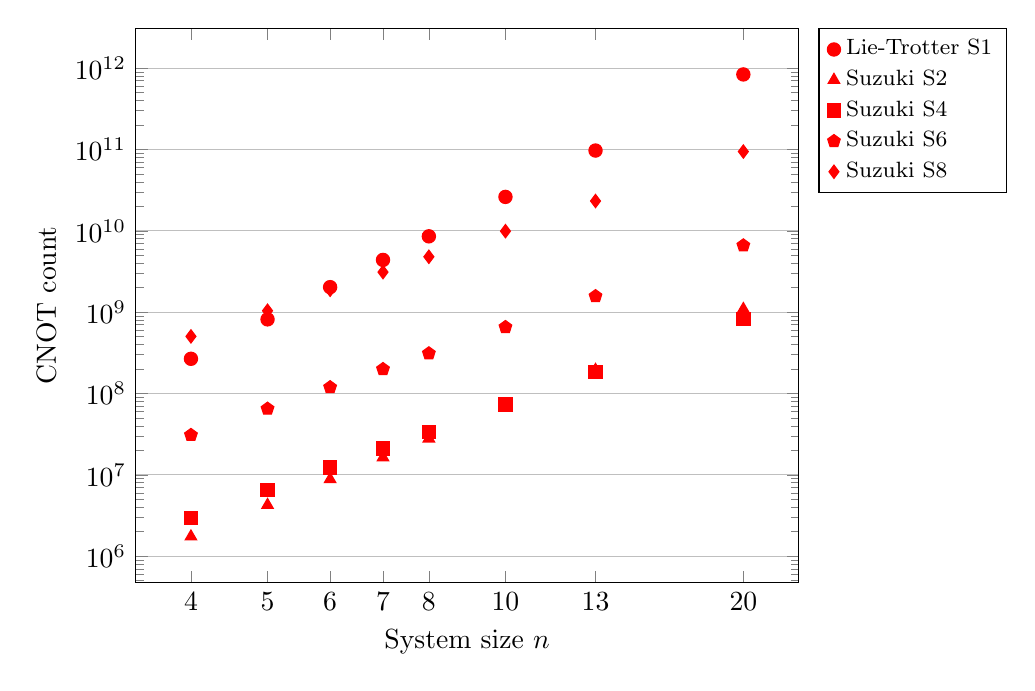
\begin{tikzpicture}
  \begin{loglogaxis}[
    width=10cm,
    xlabel={System size $n$},
    ylabel={CNOT count},
    xtick={4,5,6,7,8,10,13,20},
    xticklabels={4,5,6,7,8,10,13,20},
    ymajorgrids=true,
    legend pos=outer north east,
    legend cell align=left,
    legend style={font=\footnotesize},
  ]
    \addplot[only marks, red, mark=*, mark size=2.4pt, mark options={solid, fill=red}] coordinates {
      (4,267217992)
      (5,815484570)
      (6,2029186512)
      (7,4385871630)
      (8,8550975264)
      (10,26095505580)
      (13,96890785446)
      (20,835056177720)
    };
    \addlegendentry{Lie-Trotter S1}
    \addplot[only marks, red, mark=triangle*, mark size=2.4pt, mark options={solid, fill=red}] coordinates {
      (4,1743680)
      (5,4257000)
      (6,8827320)
      (7,16353680)
      (8,27898560)
      (10,68111700)
      (13,194533820)
      (20,1089787000)
    };
    \addlegendentry{Suzuki S2}
    \addplot[only marks, red, mark=square*, mark size=2.4pt, mark options={solid, fill=red}] coordinates {
      (4,2967216)
      (5,6479130)
      (6,12264588)
      (7,21035994)
      (8,33568752)
      (10,73302600)
      (13,183619800)
      (20,829321080)
    };
    \addlegendentry{Suzuki S4}
    \addplot[only marks, red, mark=pentagon*, mark size=2.4pt, mark options={solid, fill=red}] coordinates {
      (4,30876104)
      (5,64961180)
      (6,119286252)
      (7,199407936)
      (8,311207664)
      (10,654760780)
      (13,1569977734)
      (20,6599566240)
    };
    \addlegendentry{Suzuki S6}
    \addplot[only marks, red, mark=diamond*, mark size=2.4pt, mark options={solid, fill=red}] coordinates {
      (4,503745480)
      (5,1040321490)
      (6,1881509508)
      (7,3105153912)
      (8,4792445760)
      (10,9897255000)
      (13,23218297908)
      (20,94159022160)
    };
    \addlegendentry{Suzuki S8}
  \end{loglogaxis}
\end{tikzpicture}

\clearpage

\section*{\texttt{cnot/A-min-by-order.tex}}
Suzuki formulas of each order, r from: Minimised bound\par\medskip
% Generated by plsimcount.pffigure -- do not edit; regenerate instead.
% figure: A-min-by-order -- Suzuki formulas of each order, r from: Minimised bound
% source: results/np-main/seed1/results.json
% metric=cnot gatebase=cz merged
% seed=1 t=n template=simcount synth=pygridsynth
% git_commit=01d3c275ceae2840002bd1aaea68f59b987c4975 git_dirty=False
% source_sha256=0dd1c9775f148df550d3d3f68cfeee1d2d060b7913324535bbf1533b52b4d2c2
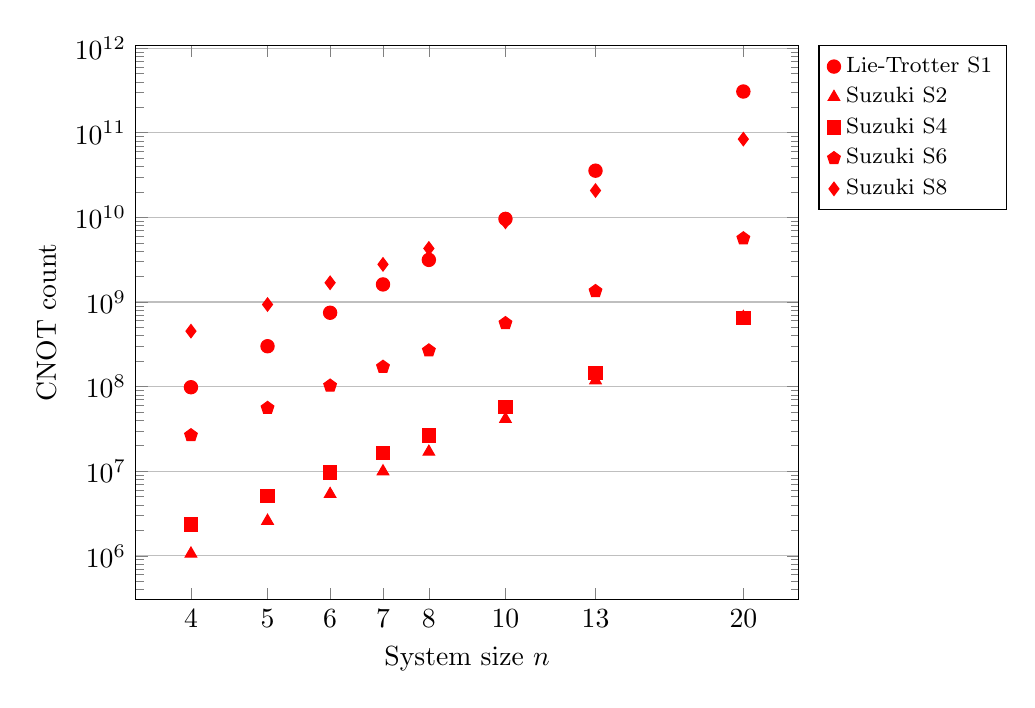
\begin{tikzpicture}
  \begin{loglogaxis}[
    width=10cm,
    xlabel={System size $n$},
    ylabel={CNOT count},
    xtick={4,5,6,7,8,10,13,20},
    xticklabels={4,5,6,7,8,10,13,20},
    ymajorgrids=true,
    legend pos=outer north east,
    legend cell align=left,
    legend style={font=\footnotesize},
  ]
    \addplot[only marks, red, mark=*, mark size=2.4pt, mark options={solid, fill=red}] coordinates {
      (4,98305536)
      (5,300003000)
      (6,746501184)
      (7,1613480232)
      (8,3145740288)
      (10,9600024000)
      (13,35644180728)
      (20,307200192000)
    };
    \addlegendentry{Lie-Trotter S1}
    \addplot[only marks, red, mark=triangle*, mark size=2.4pt, mark options={solid, fill=red}] coordinates {
      (4,1060160)
      (5,2587000)
      (6,5362680)
      (7,9932720)
      (8,16941840)
      (10,41351900)
      (13,118078610)
      (20,661309200)
    };
    \addlegendentry{Suzuki S2}
    \addplot[only marks, red, mark=square*, mark size=2.4pt, mark options={solid, fill=red}] coordinates {
      (4,2337552)
      (5,5098170)
      (6,9642024)
      (7,16526328)
      (8,26357520)
      (10,57506400)
      (13,143923416)
      (20,649227600)
    };
    \addlegendentry{Suzuki S4}
    \addplot[only marks, red, mark=pentagon*, mark size=2.4pt, mark options={solid, fill=red}] coordinates {
      (4,26563808)
      (5,55823710)
      (6,102417636)
      (7,171089758)
      (8,266856544)
      (10,560935820)
      (13,1343669054)
      (20,5640021800)
    };
    \addlegendentry{Suzuki S6}
    \addplot[only marks, red, mark=diamond*, mark size=2.4pt, mark options={solid, fill=red}] coordinates {
      (4,452499192)
      (5,933608490)
      (6,1687267800)
      (7,2782923738)
      (8,4292968800)
      (10,8858661960)
      (13,20763430974)
      (20,84091086480)
    };
    \addlegendentry{Suzuki S8}
  \end{loglogaxis}
\end{tikzpicture}

\clearpage

\section*{\texttt{cnot/A-com-by-order.tex}}
Suzuki formulas of each order, r from: Commutator bound (2018)\par\medskip
% Generated by pysimcount.pffigure -- do not edit; regenerate instead.
% figure: A-com-by-order -- Suzuki formulas of each order, r from: Commutator bound (2018)
% source: results/np-main/seed1/results.json
% metric=cnot gatebase=cz merged
% seed=1 t=n template=simcount synth=pygridsynth
% git_commit=01d3c275ceae2840002bd1aaea68f59b987c4975 git_dirty=False
% source_sha256=0dd1c9775f148df550d3d3f68cfeee1d2d060b7913324535bbf1533b52b4d2c2
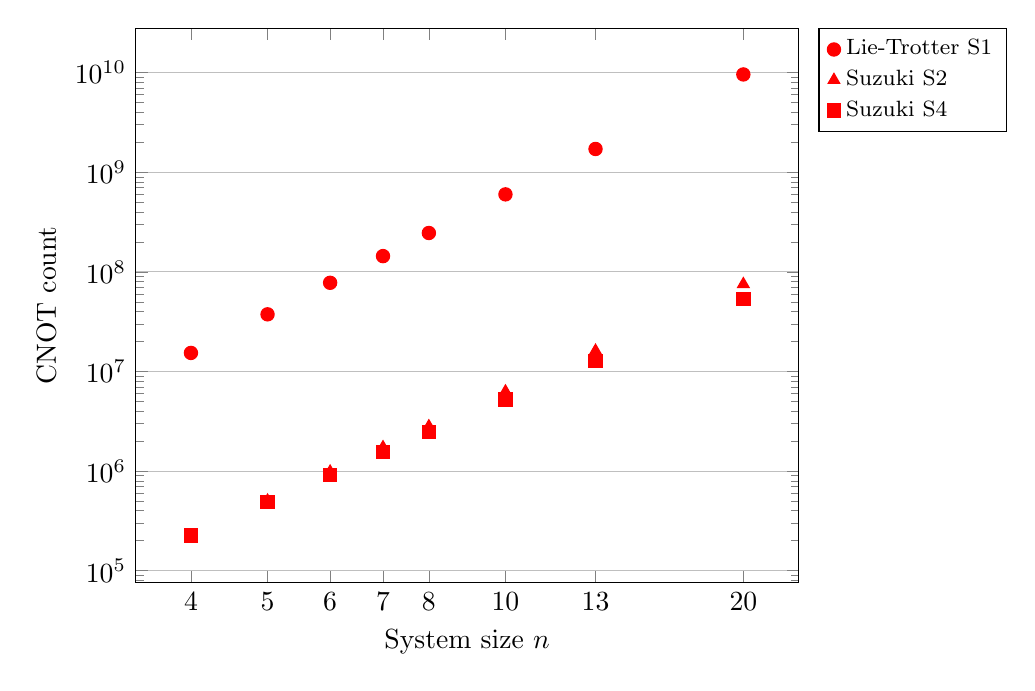
\begin{tikzpicture}
  \begin{loglogaxis}[
    width=10cm,
    xlabel={System size $n$},
    ylabel={CNOT count},
    xtick={4,5,6,7,8,10,13,20},
    xticklabels={4,5,6,7,8,10,13,20},
    ymajorgrids=true,
    legend pos=outer north east,
    legend cell align=left,
    legend style={font=\footnotesize},
  ]
    \addplot[only marks, red, mark=*, mark size=2.4pt, mark options={solid, fill=red}] coordinates {
      (4,15363288)
      (5,37508010)
      (6,77776596)
      (7,144090744)
      (8,245812464)
      (10,600127980)
      (13,1714025586)
      (20,9602047680)
    };
    \addlegendentry{Lie-Trotter S1}
    \addplot[only marks, red, mark=triangle*, mark size=2.4pt, mark options={solid, fill=red}] coordinates {
      (4,220120)
      (5,505500)
      (6,988260)
      (7,1734180)
      (8,2815200)
      (10,6299800)
      (13,16163550)
      (20,75392000)
    };
    \addlegendentry{Suzuki S2}
    \addplot[only marks, red, mark=square*, mark size=2.4pt, mark options={solid, fill=red}] coordinates {
      (4,226632)
      (5,490350)
      (6,918288)
      (7,1557612)
      (8,2457504)
      (10,5243700)
      (13,12704328)
      (20,53642400)
    };
    \addlegendentry{Suzuki S4}
  \end{loglogaxis}
\end{tikzpicture}

\clearpage

\section*{\texttt{cnot/A-emp-by-order.tex}}
Suzuki formulas of each order, r from: Empirical fit (2018)\par\medskip
% Generated by plsimcount.pffigure -- do not edit; regenerate instead.
% figure: A-emp-by-order -- Suzuki formulas of each order, r from: Empirical fit (2018)
% source: results/np-main/seed1/results.json
% metric=cnot gatebase=cz merged
% seed=1 t=n template=simcount synth=pygridsynth
% git_commit=01d3c275ceae2840002bd1aaea68f59b987c4975 git_dirty=False
% source_sha256=0dd1c9775f148df550d3d3f68cfeee1d2d060b7913324535bbf1533b52b4d2c2
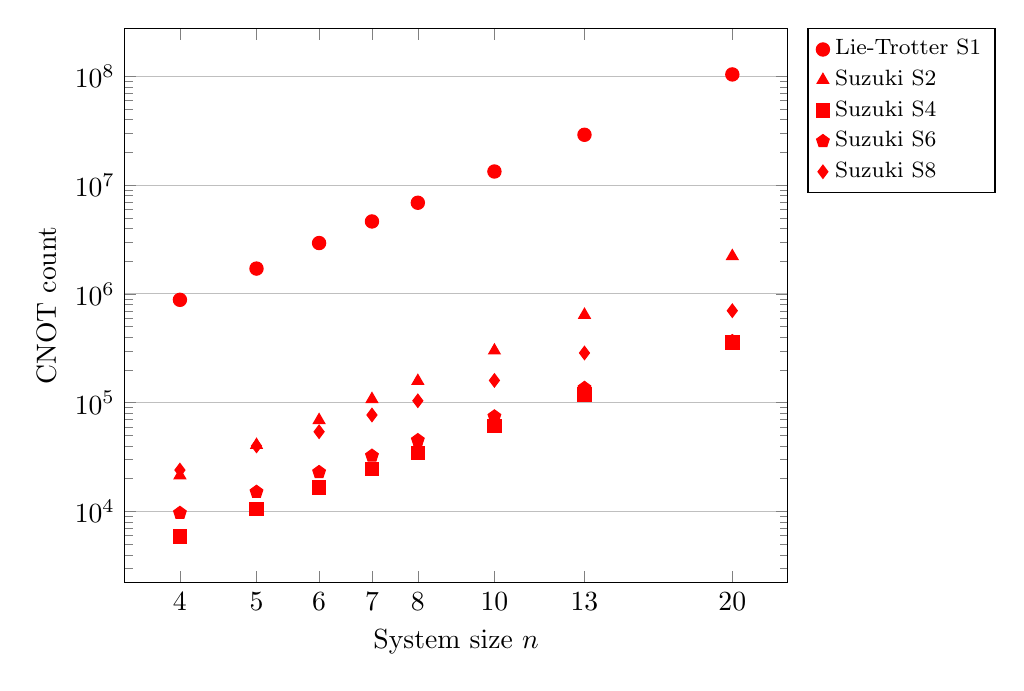
\begin{tikzpicture}
  \begin{loglogaxis}[
    width=10cm,
    xlabel={System size $n$},
    ylabel={CNOT count},
    xtick={4,5,6,7,8,10,13,20},
    xticklabels={4,5,6,7,8,10,13,20},
    ymajorgrids=true,
    legend pos=outer north east,
    legend cell align=left,
    legend style={font=\footnotesize},
  ]
    \addplot[only marks, red, mark=*, mark size=2.4pt, mark options={solid, fill=red}] coordinates {
      (4,883056)
      (5,1710900)
      (6,2937132)
      (7,4638228)
      (8,6890304)
      (10,13350000)
      (13,29054298)
      (20,104168880)
    };
    \addlegendentry{Lie-Trotter S1}
    \addplot[only marks, red, mark=triangle*, mark size=2.4pt, mark options={solid, fill=red}] coordinates {
      (4,21480)
      (5,40850)
      (6,69120)
      (7,107800)
      (8,158400)
      (10,301300)
      (13,641810)
      (20,2221800)
    };
    \addlegendentry{Suzuki S2}
    \addplot[only marks, red, mark=square*, mark size=2.4pt, mark options={solid, fill=red}] coordinates {
      (4,5880)
      (5,10500)
      (6,16632)
      (7,24696)
      (8,34608)
      (10,60900)
      (13,119028)
      (20,357000)
    };
    \addlegendentry{Suzuki S4}
    \addplot[only marks, red, mark=pentagon*, mark size=2.4pt, mark options={solid, fill=red}] coordinates {
      (4,9696)
      (5,15150)
      (6,23028)
      (7,32522)
      (8,45248)
      (10,74740)
      (13,136552)
      (20,367640)
    };
    \addlegendentry{Suzuki S6}
    \addplot[only marks, red, mark=diamond*, mark size=2.4pt, mark options={solid, fill=red}] coordinates {
      (4,24048)
      (5,40080)
      (6,54108)
      (7,77154)
      (8,104208)
      (10,160320)
      (13,286572)
      (20,701400)
    };
    \addlegendentry{Suzuki S8}
  \end{loglogaxis}
\end{tikzpicture}

\clearpage

\section*{\texttt{cnot/A-tte-by-order.tex}}
Suzuki formulas of each order, r from: Commutator bound (2021)\par\medskip
% Generated by plsimcount.pffigure -- do not edit; regenerate instead.
% figure: A-tte-by-order -- Suzuki formulas of each order, r from: Commutator bound (2021)
% source: results/np-main/seed1/results.json
% metric=cnot gatebase=cz merged
% seed=1 t=n template=simcount synth=pygridsynth
% git_commit=01d3c275ceae2840002bd1aaea68f59b987c4975 git_dirty=False
% source_sha256=0dd1c9775f148df550d3d3f68cfeee1d2d060b7913324535bbf1533b52b4d2c2
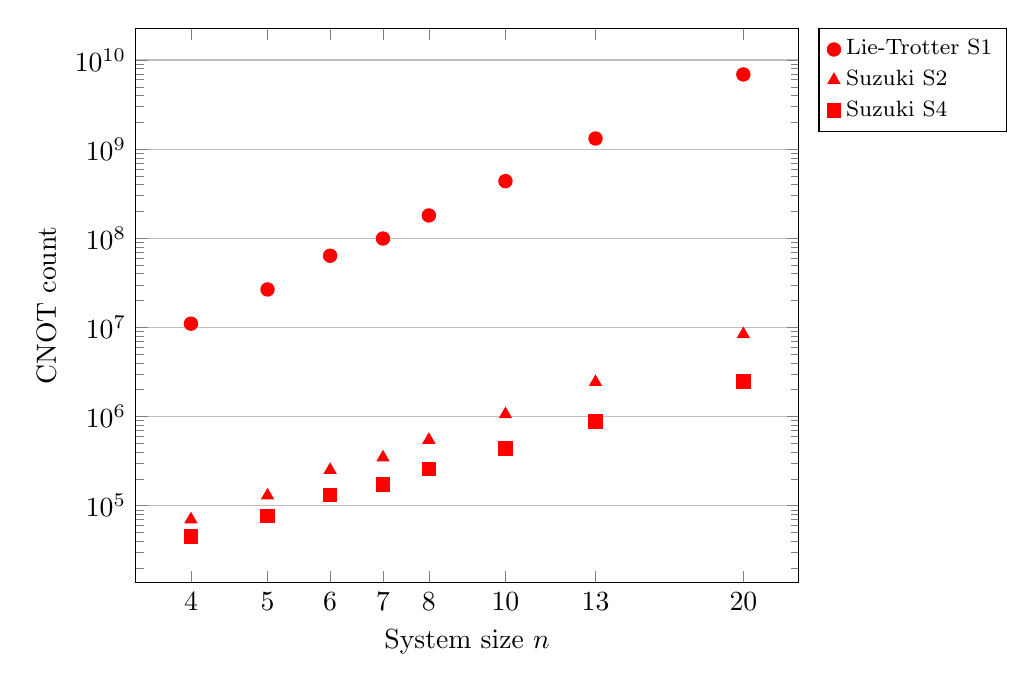
\begin{tikzpicture}
  \begin{loglogaxis}[
    width=10cm,
    xlabel={System size $n$},
    ylabel={CNOT count},
    xtick={4,5,6,7,8,10,13,20},
    xticklabels={4,5,6,7,8,10,13,20},
    ymajorgrids=true,
    legend pos=outer north east,
    legend cell align=left,
    legend style={font=\footnotesize},
  ]
    \addplot[only marks, red, mark=*, mark size=2.4pt, mark options={solid, fill=red}] coordinates {
      (4,11020296)
      (5,26672070)
      (6,63716940)
      (7,99335082)
      (8,180316560)
      (10,437836740)
      (13,1315943928)
      (20,6887318520)
    };
    \addlegendentry{Lie-Trotter S1}
    \addplot[only marks, red, mark=triangle*, mark size=2.4pt, mark options={solid, fill=red}] coordinates {
      (4,70120)
      (5,130200)
      (6,251520)
      (7,347830)
      (8,546880)
      (10,1061300)
      (13,2436330)
      (20,8383600)
    };
    \addlegendentry{Suzuki S2}
    \addplot[only marks, red, mark=square*, mark size=2.4pt, mark options={solid, fill=red}] coordinates {
      (4,45024)
      (5,76230)
      (6,131040)
      (7,173754)
      (8,257040)
      (10,437220)
      (13,884520)
      (20,2469600)
    };
    \addlegendentry{Suzuki S4}
  \end{loglogaxis}
\end{tikzpicture}

\clearpage

\section*{\texttt{cnot/A-measured-by-order.tex}}
Suzuki formulas of each order, r from: Measured $r$\par\medskip
% Generated by pysimcount.pffigure -- do not edit; regenerate instead.
% figure: A-measured-by-order -- Suzuki formulas of each order, r from: Measured $r$
% source: results/np-main/seed1/results.json
% metric=cnot gatebase=cz merged
% seed=1 t=n template=simcount synth=pygridsynth
% git_commit=01d3c275ceae2840002bd1aaea68f59b987c4975 git_dirty=False
% source_sha256=0dd1c9775f148df550d3d3f68cfeee1d2d060b7913324535bbf1533b52b4d2c2
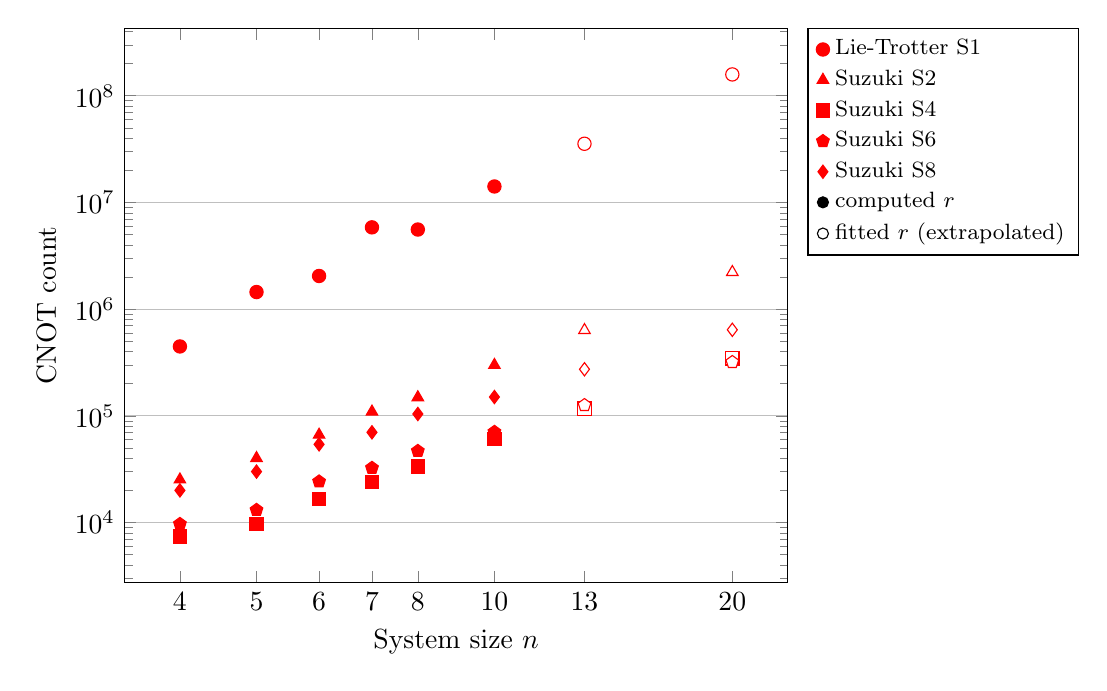
\begin{tikzpicture}
  \begin{loglogaxis}[
    width=10cm,
    xlabel={System size $n$},
    ylabel={CNOT count},
    xtick={4,5,6,7,8,10,13,20},
    xticklabels={4,5,6,7,8,10,13,20},
    ymajorgrids=true,
    legend pos=outer north east,
    legend cell align=left,
    legend style={font=\footnotesize},
  ]
    \addplot[only marks, red, mark=*, mark size=2.4pt, mark options={solid, fill=red}] coordinates {
      (4,447624)
      (5,1447710)
      (6,2047752)
      (7,5847576)
      (8,5578704)
      (10,14127480)
    };
    \addlegendentry{Lie-Trotter S1}
    % r from power-law fit (extrapolation); one legend entry per series
    \addplot[only marks, red, mark=*, mark size=2.4pt, mark options={solid, fill=white}, forget plot] coordinates {
      (13,35519406)
      (20,158501280)
    };
    \addplot[only marks, red, mark=triangle*, mark size=2.4pt, mark options={solid, fill=red}] coordinates {
      (4,25280)
      (5,40150)
      (6,66420)
      (7,109410)
      (8,149040)
      (10,299400)
    };
    \addlegendentry{Suzuki S2}
    % r from power-law fit (extrapolation); one legend entry per series
    \addplot[only marks, red, mark=triangle*, mark size=2.4pt, mark options={solid, fill=white}, forget plot] coordinates {
      (13,635700)
      (20,2223800)
    };
    \addplot[only marks, red, mark=square*, mark size=2.4pt, mark options={solid, fill=red}] coordinates {
      (4,7392)
      (5,9660)
      (6,16632)
      (7,24108)
      (8,33600)
      (10,60480)
    };
    \addlegendentry{Suzuki S4}
    % r from power-law fit (extrapolation); one legend entry per series
    \addplot[only marks, red, mark=square*, mark size=2.4pt, mark options={solid, fill=white}, forget plot] coordinates {
      (13,116844)
      (20,346080)
    };
    \addplot[only marks, red, mark=pentagon*, mark size=2.4pt, mark options={solid, fill=red}] coordinates {
      (4,9696)
      (5,13130)
      (6,24240)
      (7,32522)
      (8,46864)
      (10,70700)
    };
    \addlegendentry{Suzuki S6}
    % r from power-law fit (extrapolation); one legend entry per series
    \addplot[only marks, red, mark=pentagon*, mark size=2.4pt, mark options={solid, fill=white}, forget plot] coordinates {
      (13,126048)
      (20,319160)
    };
    \addplot[only marks, red, mark=diamond*, mark size=2.4pt, mark options={solid, fill=red}] coordinates {
      (4,20040)
      (5,30060)
      (6,54108)
      (7,70140)
      (8,104208)
      (10,150300)
    };
    \addlegendentry{Suzuki S8}
    % r from power-law fit (extrapolation); one legend entry per series
    \addplot[only marks, red, mark=diamond*, mark size=2.4pt, mark options={solid, fill=white}, forget plot] coordinates {
      (13,273546)
      (20,641280)
    };
    \addlegendimage{only marks, black, mark=*, mark options={fill=black}}
    \addlegendentry{computed $r$}
    \addlegendimage{only marks, black, mark=*, mark options={fill=white}}
    \addlegendentry{fitted $r$ (extrapolated)}
  \end{loglogaxis}
\end{tikzpicture}

\clearpage

\section*{\texttt{cnot/B-order4-by-formula.tex}}
Every order-4 formula at measured r\par\medskip
% Generated by pysimcount.pffigure -- do not edit; regenerate instead.
% figure: B-order4-by-formula -- Every order-4 formula at measured r
% source: results/np-main/seed1/results.json
% metric=cnot gatebase=cz merged
% seed=1 t=n template=simcount synth=pygridsynth
% git_commit=01d3c275ceae2840002bd1aaea68f59b987c4975 git_dirty=False
% source_sha256=0dd1c9775f148df550d3d3f68cfeee1d2d060b7913324535bbf1533b52b4d2c2
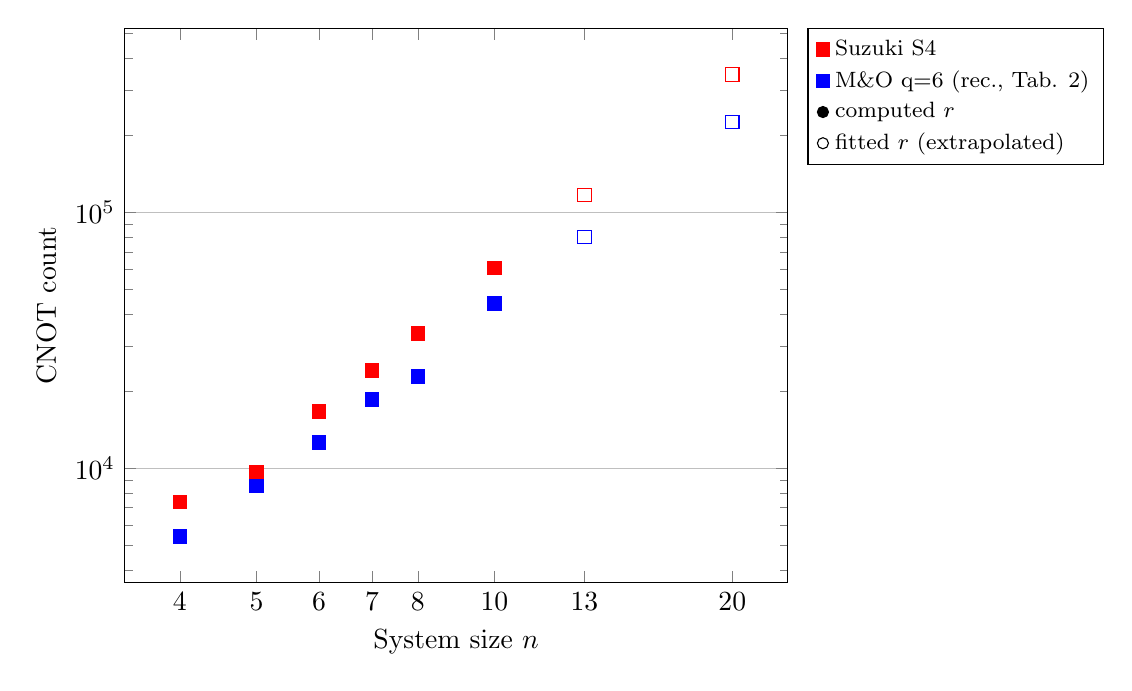
\begin{tikzpicture}
  \begin{loglogaxis}[
    width=10cm,
    xlabel={System size $n$},
    ylabel={CNOT count},
    xtick={4,5,6,7,8,10,13,20},
    xticklabels={4,5,6,7,8,10,13,20},
    ymajorgrids=true,
    legend pos=outer north east,
    legend cell align=left,
    legend style={font=\footnotesize},
  ]
    \addplot[only marks, red, mark=square*, mark size=2.4pt, mark options={solid, fill=red}] coordinates {
      (4,7392)
      (5,9660)
      (6,16632)
      (7,24108)
      (8,33600)
      (10,60480)
    };
    \addlegendentry{Suzuki S4}
    % r from power-law fit (extrapolation); one legend entry per series
    \addplot[only marks, red, mark=square*, mark size=2.4pt, mark options={solid, fill=white}, forget plot] coordinates {
      (13,116844)
      (20,346080)
    };
    \addplot[only marks, blue, mark=square*, mark size=2.4pt, mark options={solid, fill=blue}] coordinates {
      (4,5400)
      (5,8500)
      (6,12600)
      (7,18550)
      (8,22800)
      (10,44000)
    };
    \addlegendentry{M\&O q=6 (rec., Tab. 2)}
    % r from power-law fit (extrapolation); one legend entry per series
    \addplot[only marks, blue, mark=square*, mark size=2.4pt, mark options={solid, fill=white}, forget plot] coordinates {
      (13,79950)
      (20,225000)
    };
    \addlegendimage{only marks, black, mark=*, mark options={fill=black}}
    \addlegendentry{computed $r$}
    \addlegendimage{only marks, black, mark=*, mark options={fill=white}}
    \addlegendentry{fitted $r$ (extrapolated)}
  \end{loglogaxis}
\end{tikzpicture}

\clearpage

\section*{\texttt{cnot/B-order6-by-formula.tex}}
Every order-6 formula at measured r\par\medskip
% Generated by plsimcount.pffigure -- do not edit; regenerate instead.
% figure: B-order6-by-formula -- Every order-6 formula at measured r
% source: results/np-main/seed1/results.json
% metric=cnot gatebase=cz merged
% seed=1 t=n template=simcount synth=pygridsynth
% git_commit=01d3c275ceae2840002bd1aaea68f59b987c4975 git_dirty=False
% source_sha256=0dd1c9775f148df550d3d3f68cfeee1d2d060b7913324535bbf1533b52b4d2c2
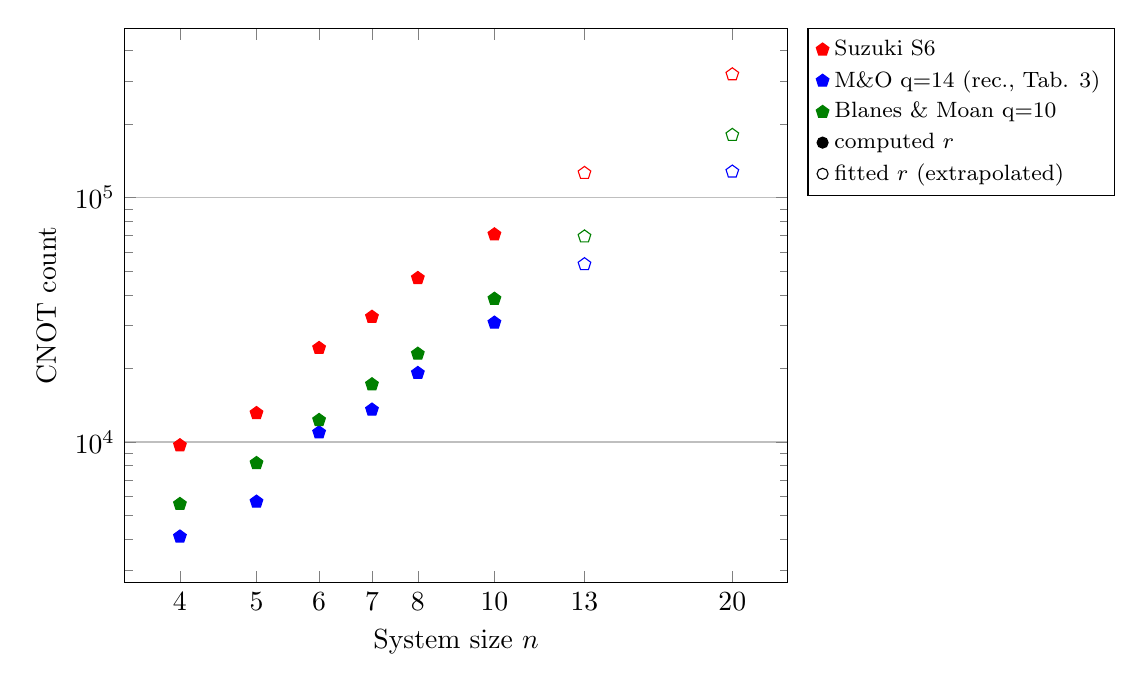
\begin{tikzpicture}
  \begin{loglogaxis}[
    width=10cm,
    xlabel={System size $n$},
    ylabel={CNOT count},
    xtick={4,5,6,7,8,10,13,20},
    xticklabels={4,5,6,7,8,10,13,20},
    ymajorgrids=true,
    legend pos=outer north east,
    legend cell align=left,
    legend style={font=\footnotesize},
  ]
    \addplot[only marks, red, mark=pentagon*, mark size=2.4pt, mark options={solid, fill=red}] coordinates {
      (4,9696)
      (5,13130)
      (6,24240)
      (7,32522)
      (8,46864)
      (10,70700)
    };
    \addlegendentry{Suzuki S6}
    % r from power-law fit (extrapolation); one legend entry per series
    \addplot[only marks, red, mark=pentagon*, mark size=2.4pt, mark options={solid, fill=white}, forget plot] coordinates {
      (13,126048)
      (20,319160)
    };
    \addplot[only marks, blue, mark=pentagon*, mark size=2.4pt, mark options={solid, fill=blue}] coordinates {
      (4,4104)
      (5,5700)
      (6,10944)
      (7,13566)
      (8,19152)
      (10,30780)
    };
    \addlegendentry{M\&O q=14 (rec., Tab. 3)}
    % r from power-law fit (extrapolation); one legend entry per series
    \addplot[only marks, blue, mark=pentagon*, mark size=2.4pt, mark options={solid, fill=white}, forget plot] coordinates {
      (13,53352)
      (20,127680)
    };
    \addplot[only marks, green!50!black, mark=pentagon*, mark size=2.4pt, mark options={solid, fill=green!50!black}] coordinates {
      (4,5576)
      (5,8200)
      (6,12300)
      (7,17220)
      (8,22960)
      (10,38540)
    };
    \addlegendentry{Blanes \& Moan q=10}
    % r from power-law fit (extrapolation); one legend entry per series
    \addplot[only marks, green!50!black, mark=pentagon*, mark size=2.4pt, mark options={solid, fill=white}, forget plot] coordinates {
      (13,69290)
      (20,180400)
    };
    \addlegendimage{only marks, black, mark=*, mark options={fill=black}}
    \addlegendentry{computed $r$}
    \addlegendimage{only marks, black, mark=*, mark options={fill=white}}
    \addlegendentry{fitted $r$ (extrapolated)}
  \end{loglogaxis}
\end{tikzpicture}

\clearpage

\section*{\texttt{cnot/B-order8-by-formula.tex}}
Every order-8 formula at measured r\par\medskip
% Generated by plsimcount.pffigure -- do not edit; regenerate instead.
% figure: B-order8-by-formula -- Every order-8 formula at measured r
% source: results/np-main/seed1/results.json
% metric=cnot gatebase=cz merged
% seed=1 t=n template=simcount synth=pygridsynth
% git_commit=01d3c275ceae2840002bd1aaea68f59b987c4975 git_dirty=False
% source_sha256=0dd1c9775f148df550d3d3f68cfeee1d2d060b7913324535bbf1533b52b4d2c2
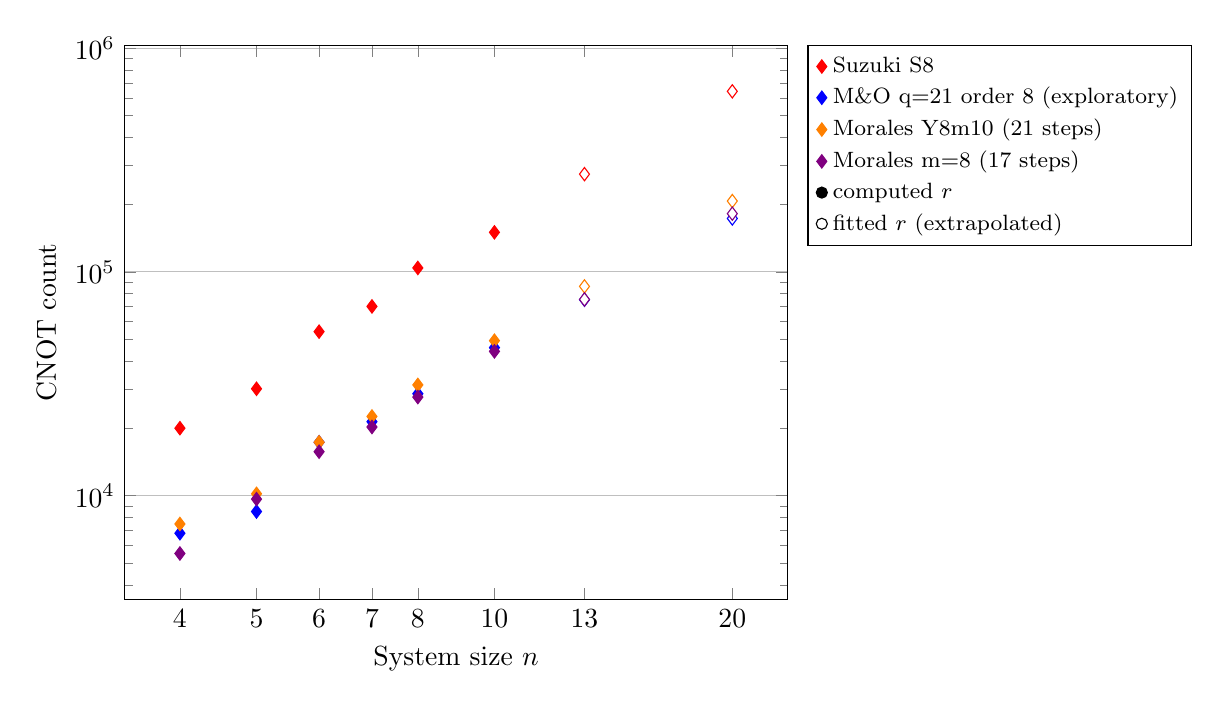
\begin{tikzpicture}
  \begin{loglogaxis}[
    width=10cm,
    xlabel={System size $n$},
    ylabel={CNOT count},
    xtick={4,5,6,7,8,10,13,20},
    xticklabels={4,5,6,7,8,10,13,20},
    ymajorgrids=true,
    legend pos=outer north east,
    legend cell align=left,
    legend style={font=\footnotesize},
  ]
    \addplot[only marks, red, mark=diamond*, mark size=2.4pt, mark options={solid, fill=red}] coordinates {
      (4,20040)
      (5,30060)
      (6,54108)
      (7,70140)
      (8,104208)
      (10,150300)
    };
    \addlegendentry{Suzuki S8}
    % r from power-law fit (extrapolation); one legend entry per series
    \addplot[only marks, red, mark=diamond*, mark size=2.4pt, mark options={solid, fill=white}, forget plot] coordinates {
      (13,273546)
      (20,641280)
    };
    \addplot[only marks, blue, mark=diamond*, mark size=2.4pt, mark options={solid, fill=blue}] coordinates {
      (4,6800)
      (5,8500)
      (6,17340)
      (7,21420)
      (8,28560)
      (10,45900)
    };
    \addlegendentry{M\&O q=21 order 8 (exploratory)}
    % r from power-law fit (extrapolation); one legend entry per series
    \addplot[only marks, blue, mark=diamond*, mark size=2.4pt, mark options={solid, fill=white}, forget plot] coordinates {
      (13,75140)
      (20,173400)
    };
    \addplot[only marks, orange, mark=diamond*, mark size=2.4pt, mark options={solid, fill=orange}] coordinates {
      (4,7480)
      (5,10200)
      (6,17340)
      (7,22610)
      (8,31280)
      (10,49300)
    };
    \addlegendentry{Morales Y8m10 (21 steps)}
    % r from power-law fit (extrapolation); one legend entry per series
    \addplot[only marks, orange, mark=diamond*, mark size=2.4pt, mark options={solid, fill=white}, forget plot] coordinates {
      (13,86190)
      (20,207400)
    };
    \addplot[only marks, violet, mark=diamond*, mark size=2.4pt, mark options={solid, fill=violet}] coordinates {
      (4,5520)
      (5,9660)
      (6,15732)
      (7,20286)
      (8,27600)
      (10,44160)
    };
    \addlegendentry{Morales m=8 (17 steps)}
    % r from power-law fit (extrapolation); one legend entry per series
    \addplot[only marks, violet, mark=diamond*, mark size=2.4pt, mark options={solid, fill=white}, forget plot] coordinates {
      (13,75348)
      (20,182160)
    };
    \addlegendimage{only marks, black, mark=*, mark options={fill=black}}
    \addlegendentry{computed $r$}
    \addlegendimage{only marks, black, mark=*, mark options={fill=white}}
    \addlegendentry{fitted $r$ (extrapolated)}
  \end{loglogaxis}
\end{tikzpicture}

\clearpage

\section*{\texttt{cnot/B-all-by-formula.tex}}
Every formula at measured r\par\medskip
% Generated by pysimcount.pffigure -- do not edit; regenerate instead.
% figure: B-all-by-formula -- Every formula at measured r
% source: results/np-main/seed1/results.json
% metric=cnot gatebase=cz merged
% seed=1 t=n template=simcount synth=pygridsynth
% git_commit=01d3c275ceae2840002bd1aaea68f59b987c4975 git_dirty=False
% source_sha256=0dd1c9775f148df550d3d3f68cfeee1d2d060b7913324535bbf1533b52b4d2c2
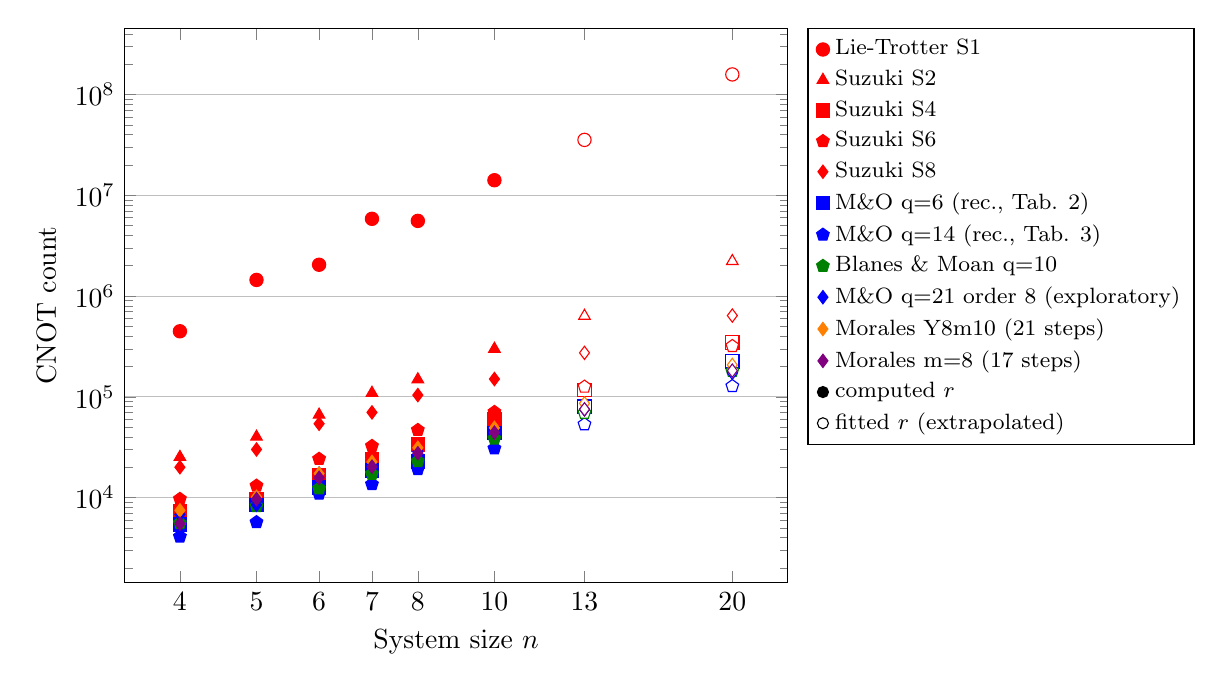
\begin{tikzpicture}
  \begin{loglogaxis}[
    width=10cm,
    xlabel={System size $n$},
    ylabel={CNOT count},
    xtick={4,5,6,7,8,10,13,20},
    xticklabels={4,5,6,7,8,10,13,20},
    ymajorgrids=true,
    legend pos=outer north east,
    legend cell align=left,
    legend style={font=\footnotesize},
  ]
    \addplot[only marks, red, mark=*, mark size=2.4pt, mark options={solid, fill=red}] coordinates {
      (4,447624)
      (5,1447710)
      (6,2047752)
      (7,5847576)
      (8,5578704)
      (10,14127480)
    };
    \addlegendentry{Lie-Trotter S1}
    % r from power-law fit (extrapolation); one legend entry per series
    \addplot[only marks, red, mark=*, mark size=2.4pt, mark options={solid, fill=white}, forget plot] coordinates {
      (13,35519406)
      (20,158501280)
    };
    \addplot[only marks, red, mark=triangle*, mark size=2.4pt, mark options={solid, fill=red}] coordinates {
      (4,25280)
      (5,40150)
      (6,66420)
      (7,109410)
      (8,149040)
      (10,299400)
    };
    \addlegendentry{Suzuki S2}
    % r from power-law fit (extrapolation); one legend entry per series
    \addplot[only marks, red, mark=triangle*, mark size=2.4pt, mark options={solid, fill=white}, forget plot] coordinates {
      (13,635700)
      (20,2223800)
    };
    \addplot[only marks, red, mark=square*, mark size=2.4pt, mark options={solid, fill=red}] coordinates {
      (4,7392)
      (5,9660)
      (6,16632)
      (7,24108)
      (8,33600)
      (10,60480)
    };
    \addlegendentry{Suzuki S4}
    % r from power-law fit (extrapolation); one legend entry per series
    \addplot[only marks, red, mark=square*, mark size=2.4pt, mark options={solid, fill=white}, forget plot] coordinates {
      (13,116844)
      (20,346080)
    };
    \addplot[only marks, red, mark=pentagon*, mark size=2.4pt, mark options={solid, fill=red}] coordinates {
      (4,9696)
      (5,13130)
      (6,24240)
      (7,32522)
      (8,46864)
      (10,70700)
    };
    \addlegendentry{Suzuki S6}
    % r from power-law fit (extrapolation); one legend entry per series
    \addplot[only marks, red, mark=pentagon*, mark size=2.4pt, mark options={solid, fill=white}, forget plot] coordinates {
      (13,126048)
      (20,319160)
    };
    \addplot[only marks, red, mark=diamond*, mark size=2.4pt, mark options={solid, fill=red}] coordinates {
      (4,20040)
      (5,30060)
      (6,54108)
      (7,70140)
      (8,104208)
      (10,150300)
    };
    \addlegendentry{Suzuki S8}
    % r from power-law fit (extrapolation); one legend entry per series
    \addplot[only marks, red, mark=diamond*, mark size=2.4pt, mark options={solid, fill=white}, forget plot] coordinates {
      (13,273546)
      (20,641280)
    };
    \addplot[only marks, blue, mark=square*, mark size=2.4pt, mark options={solid, fill=blue}] coordinates {
      (4,5400)
      (5,8500)
      (6,12600)
      (7,18550)
      (8,22800)
      (10,44000)
    };
    \addlegendentry{M\&O q=6 (rec., Tab. 2)}
    % r from power-law fit (extrapolation); one legend entry per series
    \addplot[only marks, blue, mark=square*, mark size=2.4pt, mark options={solid, fill=white}, forget plot] coordinates {
      (13,79950)
      (20,225000)
    };
    \addplot[only marks, blue, mark=pentagon*, mark size=2.4pt, mark options={solid, fill=blue}] coordinates {
      (4,4104)
      (5,5700)
      (6,10944)
      (7,13566)
      (8,19152)
      (10,30780)
    };
    \addlegendentry{M\&O q=14 (rec., Tab. 3)}
    % r from power-law fit (extrapolation); one legend entry per series
    \addplot[only marks, blue, mark=pentagon*, mark size=2.4pt, mark options={solid, fill=white}, forget plot] coordinates {
      (13,53352)
      (20,127680)
    };
    \addplot[only marks, green!50!black, mark=pentagon*, mark size=2.4pt, mark options={solid, fill=green!50!black}] coordinates {
      (4,5576)
      (5,8200)
      (6,12300)
      (7,17220)
      (8,22960)
      (10,38540)
    };
    \addlegendentry{Blanes \& Moan q=10}
    % r from power-law fit (extrapolation); one legend entry per series
    \addplot[only marks, green!50!black, mark=pentagon*, mark size=2.4pt, mark options={solid, fill=white}, forget plot] coordinates {
      (13,69290)
      (20,180400)
    };
    \addplot[only marks, blue, mark=diamond*, mark size=2.4pt, mark options={solid, fill=blue}] coordinates {
      (4,6800)
      (5,8500)
      (6,17340)
      (7,21420)
      (8,28560)
      (10,45900)
    };
    \addlegendentry{M\&O q=21 order 8 (exploratory)}
    % r from power-law fit (extrapolation); one legend entry per series
    \addplot[only marks, blue, mark=diamond*, mark size=2.4pt, mark options={solid, fill=white}, forget plot] coordinates {
      (13,75140)
      (20,173400)
    };
    \addplot[only marks, orange, mark=diamond*, mark size=2.4pt, mark options={solid, fill=orange}] coordinates {
      (4,7480)
      (5,10200)
      (6,17340)
      (7,22610)
      (8,31280)
      (10,49300)
    };
    \addlegendentry{Morales Y8m10 (21 steps)}
    % r from power-law fit (extrapolation); one legend entry per series
    \addplot[only marks, orange, mark=diamond*, mark size=2.4pt, mark options={solid, fill=white}, forget plot] coordinates {
      (13,86190)
      (20,207400)
    };
    \addplot[only marks, violet, mark=diamond*, mark size=2.4pt, mark options={solid, fill=violet}] coordinates {
      (4,5520)
      (5,9660)
      (6,15732)
      (7,20286)
      (8,27600)
      (10,44160)
    };
    \addlegendentry{Morales m=8 (17 steps)}
    % r from power-law fit (extrapolation); one legend entry per series
    \addplot[only marks, violet, mark=diamond*, mark size=2.4pt, mark options={solid, fill=white}, forget plot] coordinates {
      (13,75348)
      (20,182160)
    };
    \addlegendimage{only marks, black, mark=*, mark options={fill=black}}
    \addlegendentry{computed $r$}
    \addlegendimage{only marks, black, mark=*, mark options={fill=white}}
    \addlegendentry{fitted $r$ (extrapolated)}
  \end{loglogaxis}
\end{tikzpicture}

\clearpage

\section*{\texttt{cnot/C-lie-trotter-by-bound.tex}}
Lie-Trotter S1: r from each bound and measured\par\medskip
% Generated by plsimcount.pffigure -- do not edit; regenerate instead.
% figure: C-lie-trotter-by-bound -- Lie-Trotter S1: r from each bound and measured
% source: results/np-main/seed1/results.json
% metric=cnot gatebase=cz merged
% seed=1 t=n template=simcount synth=pygridsynth
% git_commit=01d3c275ceae2840002bd1aaea68f59b987c4975 git_dirty=False
% source_sha256=0dd1c9775f148df550d3d3f68cfeee1d2d060b7913324535bbf1533b52b4d2c2
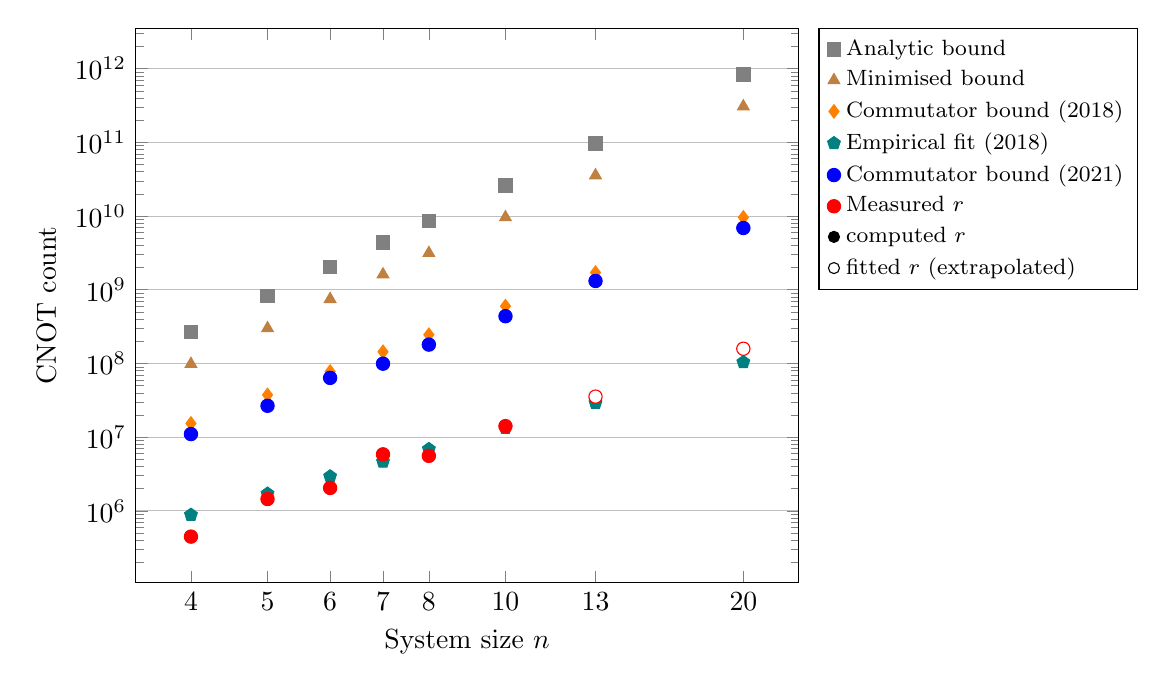
\begin{tikzpicture}
  \begin{loglogaxis}[
    width=10cm,
    xlabel={System size $n$},
    ylabel={CNOT count},
    xtick={4,5,6,7,8,10,13,20},
    xticklabels={4,5,6,7,8,10,13,20},
    ymajorgrids=true,
    legend pos=outer north east,
    legend cell align=left,
    legend style={font=\footnotesize},
  ]
    \addplot[only marks, gray, mark=square*, mark size=2.4pt, mark options={solid, fill=gray}] coordinates {
      (4,267217992)
      (5,815484570)
      (6,2029186512)
      (7,4385871630)
      (8,8550975264)
      (10,26095505580)
      (13,96890785446)
      (20,835056177720)
    };
    \addlegendentry{Analytic bound}
    \addplot[only marks, brown, mark=triangle*, mark size=2.4pt, mark options={solid, fill=brown}] coordinates {
      (4,98305536)
      (5,300003000)
      (6,746501184)
      (7,1613480232)
      (8,3145740288)
      (10,9600024000)
      (13,35644180728)
      (20,307200192000)
    };
    \addlegendentry{Minimised bound}
    \addplot[only marks, orange, mark=diamond*, mark size=2.4pt, mark options={solid, fill=orange}] coordinates {
      (4,15363288)
      (5,37508010)
      (6,77776596)
      (7,144090744)
      (8,245812464)
      (10,600127980)
      (13,1714025586)
      (20,9602047680)
    };
    \addlegendentry{Commutator bound (2018)}
    \addplot[only marks, teal, mark=pentagon*, mark size=2.4pt, mark options={solid, fill=teal}] coordinates {
      (4,883056)
      (5,1710900)
      (6,2937132)
      (7,4638228)
      (8,6890304)
      (10,13350000)
      (13,29054298)
      (20,104168880)
    };
    \addlegendentry{Empirical fit (2018)}
    \addplot[only marks, blue, mark=oplus*, mark size=2.4pt, mark options={solid, fill=blue}] coordinates {
      (4,11020296)
      (5,26672070)
      (6,63716940)
      (7,99335082)
      (8,180316560)
      (10,437836740)
      (13,1315943928)
      (20,6887318520)
    };
    \addlegendentry{Commutator bound (2021)}
    \addplot[only marks, red, mark=*, mark size=2.4pt, mark options={solid, fill=red}] coordinates {
      (4,447624)
      (5,1447710)
      (6,2047752)
      (7,5847576)
      (8,5578704)
      (10,14127480)
    };
    \addlegendentry{Measured $r$}
    % r from power-law fit (extrapolation); one legend entry per series
    \addplot[only marks, red, mark=*, mark size=2.4pt, mark options={solid, fill=white}, forget plot] coordinates {
      (13,35519406)
      (20,158501280)
    };
    \addlegendimage{only marks, black, mark=*, mark options={fill=black}}
    \addlegendentry{computed $r$}
    \addlegendimage{only marks, black, mark=*, mark options={fill=white}}
    \addlegendentry{fitted $r$ (extrapolated)}
  \end{loglogaxis}
\end{tikzpicture}

\clearpage

\section*{\texttt{cnot/C-suzuki2-by-bound.tex}}
Suzuki S2: r from each bound and measured\par\medskip
% Generated by pysimcount.pffigure -- do not edit; regenerate instead.
% figure: C-suzuki2-by-bound -- Suzuki S2: r from each bound and measured
% source: results/np-main/seed1/results.json
% metric=cnot gatebase=cz merged
% seed=1 t=n template=simcount synth=pygridsynth
% git_commit=01d3c275ceae2840002bd1aaea68f59b987c4975 git_dirty=False
% source_sha256=0dd1c9775f148df550d3d3f68cfeee1d2d060b7913324535bbf1533b52b4d2c2
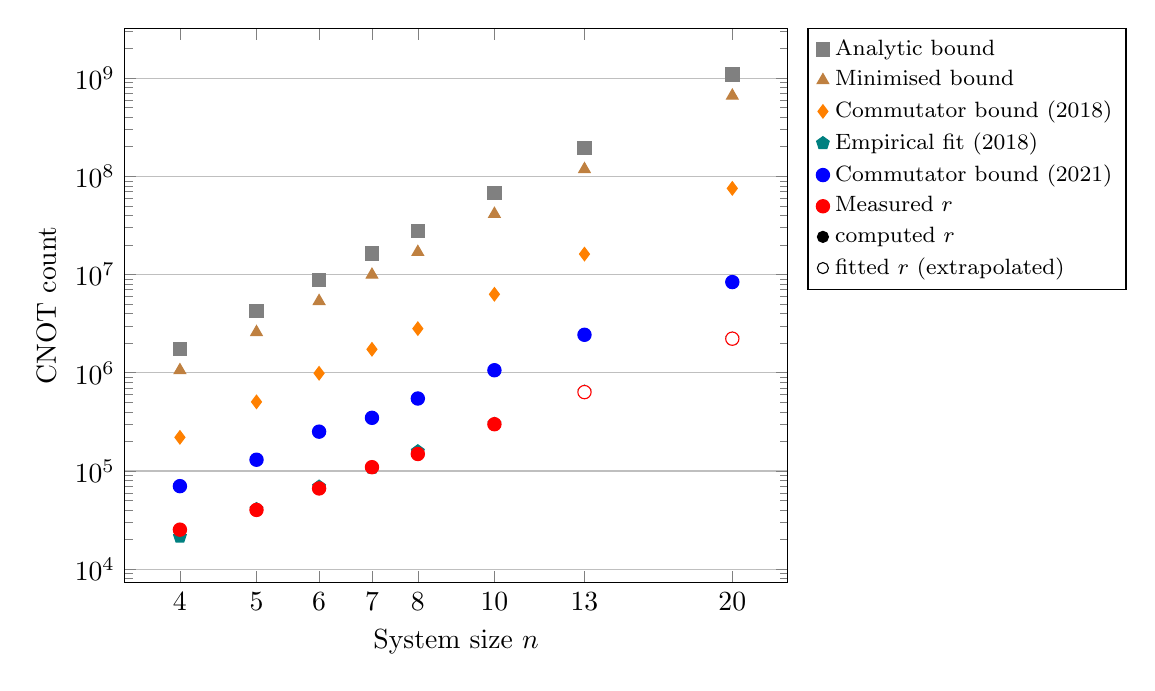
\begin{tikzpicture}
  \begin{loglogaxis}[
    width=10cm,
    xlabel={System size $n$},
    ylabel={CNOT count},
    xtick={4,5,6,7,8,10,13,20},
    xticklabels={4,5,6,7,8,10,13,20},
    ymajorgrids=true,
    legend pos=outer north east,
    legend cell align=left,
    legend style={font=\footnotesize},
  ]
    \addplot[only marks, gray, mark=square*, mark size=2.4pt, mark options={solid, fill=gray}] coordinates {
      (4,1743680)
      (5,4257000)
      (6,8827320)
      (7,16353680)
      (8,27898560)
      (10,68111700)
      (13,194533820)
      (20,1089787000)
    };
    \addlegendentry{Analytic bound}
    \addplot[only marks, brown, mark=triangle*, mark size=2.4pt, mark options={solid, fill=brown}] coordinates {
      (4,1060160)
      (5,2587000)
      (6,5362680)
      (7,9932720)
      (8,16941840)
      (10,41351900)
      (13,118078610)
      (20,661309200)
    };
    \addlegendentry{Minimised bound}
    \addplot[only marks, orange, mark=diamond*, mark size=2.4pt, mark options={solid, fill=orange}] coordinates {
      (4,220120)
      (5,505500)
      (6,988260)
      (7,1734180)
      (8,2815200)
      (10,6299800)
      (13,16163550)
      (20,75392000)
    };
    \addlegendentry{Commutator bound (2018)}
    \addplot[only marks, teal, mark=pentagon*, mark size=2.4pt, mark options={solid, fill=teal}] coordinates {
      (4,21480)
      (5,40850)
      (6,69120)
      (7,107800)
      (8,158400)
      (10,301300)
      (13,641810)
      (20,2221800)
    };
    \addlegendentry{Empirical fit (2018)}
    \addplot[only marks, blue, mark=oplus*, mark size=2.4pt, mark options={solid, fill=blue}] coordinates {
      (4,70120)
      (5,130200)
      (6,251520)
      (7,347830)
      (8,546880)
      (10,1061300)
      (13,2436330)
      (20,8383600)
    };
    \addlegendentry{Commutator bound (2021)}
    \addplot[only marks, red, mark=*, mark size=2.4pt, mark options={solid, fill=red}] coordinates {
      (4,25280)
      (5,40150)
      (6,66420)
      (7,109410)
      (8,149040)
      (10,299400)
    };
    \addlegendentry{Measured $r$}
    % r from power-law fit (extrapolation); one legend entry per series
    \addplot[only marks, red, mark=*, mark size=2.4pt, mark options={solid, fill=white}, forget plot] coordinates {
      (13,635700)
      (20,2223800)
    };
    \addlegendimage{only marks, black, mark=*, mark options={fill=black}}
    \addlegendentry{computed $r$}
    \addlegendimage{only marks, black, mark=*, mark options={fill=white}}
    \addlegendentry{fitted $r$ (extrapolated)}
  \end{loglogaxis}
\end{tikzpicture}

\clearpage

\section*{\texttt{cnot/C-suzuki4-by-bound.tex}}
Suzuki S4: r from each bound and measured\par\medskip
% Generated by pysimcount.pffigure -- do not edit; regenerate instead.
% figure: C-suzuki4-by-bound -- Suzuki S4: r from each bound and measured
% source: results/np-main/seed1/results.json
% metric=cnot gatebase=cz merged
% seed=1 t=n template=simcount synth=pygridsynth
% git_commit=01d3c275ceae2840002bd1aaea68f59b987c4975 git_dirty=False
% source_sha256=0dd1c9775f148df550d3d3f68cfeee1d2d060b7913324535bbf1533b52b4d2c2
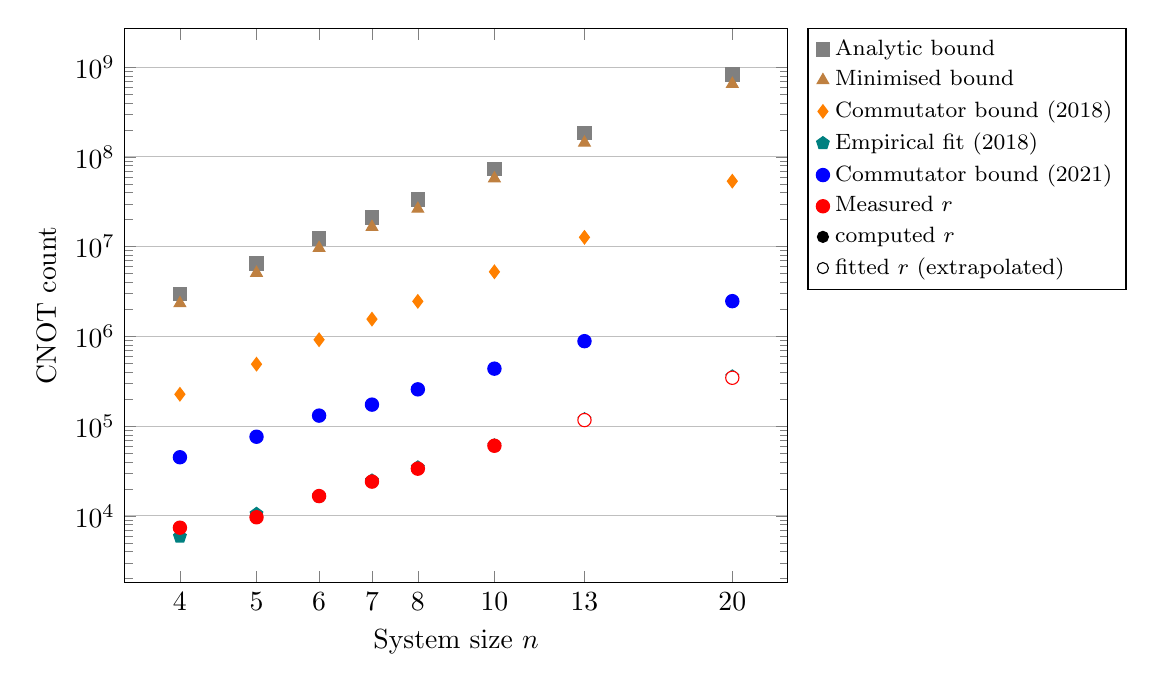
\begin{tikzpicture}
  \begin{loglogaxis}[
    width=10cm,
    xlabel={System size $n$},
    ylabel={CNOT count},
    xtick={4,5,6,7,8,10,13,20},
    xticklabels={4,5,6,7,8,10,13,20},
    ymajorgrids=true,
    legend pos=outer north east,
    legend cell align=left,
    legend style={font=\footnotesize},
  ]
    \addplot[only marks, gray, mark=square*, mark size=2.4pt, mark options={solid, fill=gray}] coordinates {
      (4,2967216)
      (5,6479130)
      (6,12264588)
      (7,21035994)
      (8,33568752)
      (10,73302600)
      (13,183619800)
      (20,829321080)
    };
    \addlegendentry{Analytic bound}
    \addplot[only marks, brown, mark=triangle*, mark size=2.4pt, mark options={solid, fill=brown}] coordinates {
      (4,2337552)
      (5,5098170)
      (6,9642024)
      (7,16526328)
      (8,26357520)
      (10,57506400)
      (13,143923416)
      (20,649227600)
    };
    \addlegendentry{Minimised bound}
    \addplot[only marks, orange, mark=diamond*, mark size=2.4pt, mark options={solid, fill=orange}] coordinates {
      (4,226632)
      (5,490350)
      (6,918288)
      (7,1557612)
      (8,2457504)
      (10,5243700)
      (13,12704328)
      (20,53642400)
    };
    \addlegendentry{Commutator bound (2018)}
    \addplot[only marks, teal, mark=pentagon*, mark size=2.4pt, mark options={solid, fill=teal}] coordinates {
      (4,5880)
      (5,10500)
      (6,16632)
      (7,24696)
      (8,34608)
      (10,60900)
      (13,119028)
      (20,357000)
    };
    \addlegendentry{Empirical fit (2018)}
    \addplot[only marks, blue, mark=oplus*, mark size=2.4pt, mark options={solid, fill=blue}] coordinates {
      (4,45024)
      (5,76230)
      (6,131040)
      (7,173754)
      (8,257040)
      (10,437220)
      (13,884520)
      (20,2469600)
    };
    \addlegendentry{Commutator bound (2021)}
    \addplot[only marks, red, mark=*, mark size=2.4pt, mark options={solid, fill=red}] coordinates {
      (4,7392)
      (5,9660)
      (6,16632)
      (7,24108)
      (8,33600)
      (10,60480)
    };
    \addlegendentry{Measured $r$}
    % r from power-law fit (extrapolation); one legend entry per series
    \addplot[only marks, red, mark=*, mark size=2.4pt, mark options={solid, fill=white}, forget plot] coordinates {
      (13,116844)
      (20,346080)
    };
    \addlegendimage{only marks, black, mark=*, mark options={fill=black}}
    \addlegendentry{computed $r$}
    \addlegendimage{only marks, black, mark=*, mark options={fill=white}}
    \addlegendentry{fitted $r$ (extrapolated)}
  \end{loglogaxis}
\end{tikzpicture}

\clearpage

\section*{\texttt{cnot/C-suzuki6-by-bound.tex}}
Suzuki S6: r from each bound and measured\par\medskip
% Generated by pysimcount.pffigure -- do not edit; regenerate instead.
% figure: C-suzuki6-by-bound -- Suzuki S6: r from each bound and measured
% source: results/np-main/seed1/results.json
% metric=cnot gatebase=cz merged
% seed=1 t=n template=simcount synth=pygridsynth
% git_commit=01d3c275ceae2840002bd1aaea68f59b987c4975 git_dirty=False
% source_sha256=0dd1c9775f148df550d3d3f68cfeee1d2d060b7913324535bbf1533b52b4d2c2
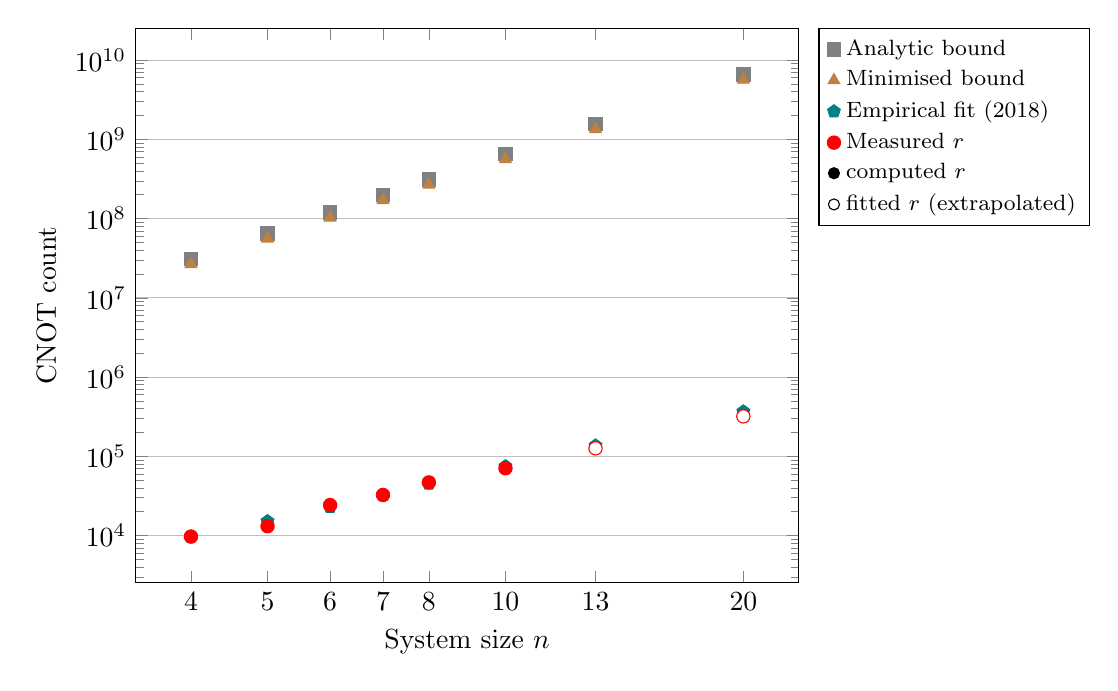
\begin{tikzpicture}
  \begin{loglogaxis}[
    width=10cm,
    xlabel={System size $n$},
    ylabel={CNOT count},
    xtick={4,5,6,7,8,10,13,20},
    xticklabels={4,5,6,7,8,10,13,20},
    ymajorgrids=true,
    legend pos=outer north east,
    legend cell align=left,
    legend style={font=\footnotesize},
  ]
    \addplot[only marks, gray, mark=square*, mark size=2.4pt, mark options={solid, fill=gray}] coordinates {
      (4,30876104)
      (5,64961180)
      (6,119286252)
      (7,199407936)
      (8,311207664)
      (10,654760780)
      (13,1569977734)
      (20,6599566240)
    };
    \addlegendentry{Analytic bound}
    \addplot[only marks, brown, mark=triangle*, mark size=2.4pt, mark options={solid, fill=brown}] coordinates {
      (4,26563808)
      (5,55823710)
      (6,102417636)
      (7,171089758)
      (8,266856544)
      (10,560935820)
      (13,1343669054)
      (20,5640021800)
    };
    \addlegendentry{Minimised bound}
    \addplot[only marks, teal, mark=pentagon*, mark size=2.4pt, mark options={solid, fill=teal}] coordinates {
      (4,9696)
      (5,15150)
      (6,23028)
      (7,32522)
      (8,45248)
      (10,74740)
      (13,136552)
      (20,367640)
    };
    \addlegendentry{Empirical fit (2018)}
    \addplot[only marks, red, mark=*, mark size=2.4pt, mark options={solid, fill=red}] coordinates {
      (4,9696)
      (5,13130)
      (6,24240)
      (7,32522)
      (8,46864)
      (10,70700)
    };
    \addlegendentry{Measured $r$}
    % r from power-law fit (extrapolation); one legend entry per series
    \addplot[only marks, red, mark=*, mark size=2.4pt, mark options={solid, fill=white}, forget plot] coordinates {
      (13,126048)
      (20,319160)
    };
    \addlegendimage{only marks, black, mark=*, mark options={fill=black}}
    \addlegendentry{computed $r$}
    \addlegendimage{only marks, black, mark=*, mark options={fill=white}}
    \addlegendentry{fitted $r$ (extrapolated)}
  \end{loglogaxis}
\end{tikzpicture}

\clearpage

\section*{\texttt{cnot/C-suzuki8-by-bound.tex}}
Suzuki S8: r from each bound and measured\par\medskip
% Generated by pysimcount.pffigure -- do not edit; regenerate instead.
% figure: C-suzuki8-by-bound -- Suzuki S8: r from each bound and measured
% source: results/np-main/seed1/results.json
% metric=cnot gatebase=cz merged
% seed=1 t=n template=simcount synth=pygridsynth
% git_commit=01d3c275ceae2840002bd1aaea68f59b987c4975 git_dirty=False
% source_sha256=0dd1c9775f148df550d3d3f68cfeee1d2d060b7913324535bbf1533b52b4d2c2
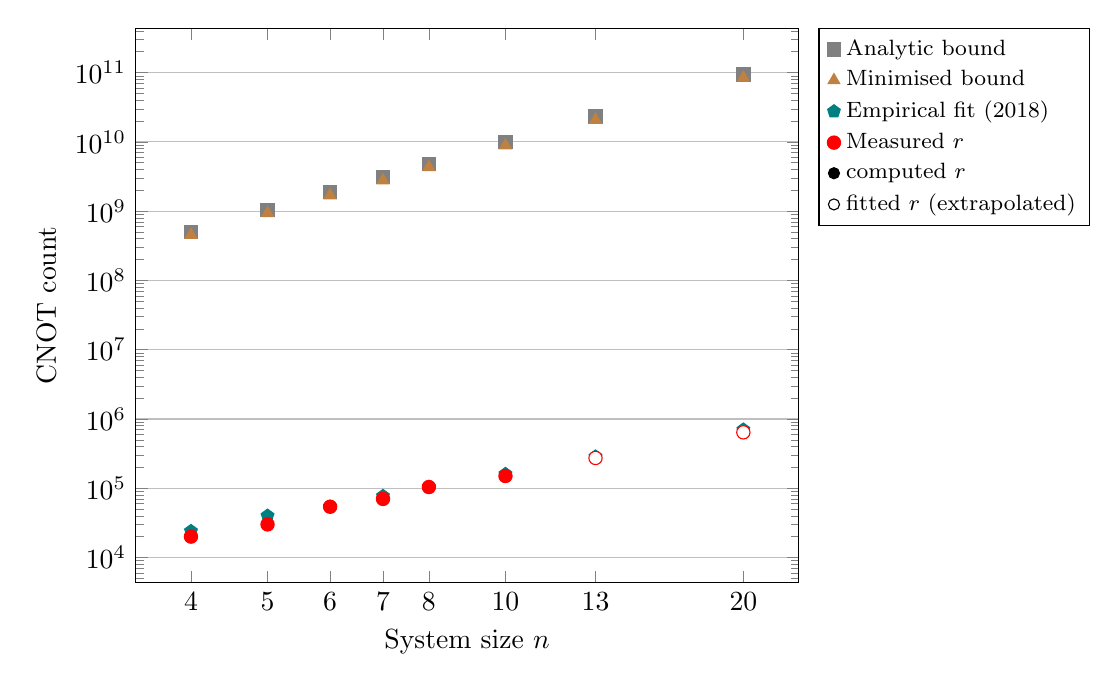
\begin{tikzpicture}
  \begin{loglogaxis}[
    width=10cm,
    xlabel={System size $n$},
    ylabel={CNOT count},
    xtick={4,5,6,7,8,10,13,20},
    xticklabels={4,5,6,7,8,10,13,20},
    ymajorgrids=true,
    legend pos=outer north east,
    legend cell align=left,
    legend style={font=\footnotesize},
  ]
    \addplot[only marks, gray, mark=square*, mark size=2.4pt, mark options={solid, fill=gray}] coordinates {
      (4,503745480)
      (5,1040321490)
      (6,1881509508)
      (7,3105153912)
      (8,4792445760)
      (10,9897255000)
      (13,23218297908)
      (20,94159022160)
    };
    \addlegendentry{Analytic bound}
    \addplot[only marks, brown, mark=triangle*, mark size=2.4pt, mark options={solid, fill=brown}] coordinates {
      (4,452499192)
      (5,933608490)
      (6,1687267800)
      (7,2782923738)
      (8,4292968800)
      (10,8858661960)
      (13,20763430974)
      (20,84091086480)
    };
    \addlegendentry{Minimised bound}
    \addplot[only marks, teal, mark=pentagon*, mark size=2.4pt, mark options={solid, fill=teal}] coordinates {
      (4,24048)
      (5,40080)
      (6,54108)
      (7,77154)
      (8,104208)
      (10,160320)
      (13,286572)
      (20,701400)
    };
    \addlegendentry{Empirical fit (2018)}
    \addplot[only marks, red, mark=*, mark size=2.4pt, mark options={solid, fill=red}] coordinates {
      (4,20040)
      (5,30060)
      (6,54108)
      (7,70140)
      (8,104208)
      (10,150300)
    };
    \addlegendentry{Measured $r$}
    % r from power-law fit (extrapolation); one legend entry per series
    \addplot[only marks, red, mark=*, mark size=2.4pt, mark options={solid, fill=white}, forget plot] coordinates {
      (13,273546)
      (20,641280)
    };
    \addlegendimage{only marks, black, mark=*, mark options={fill=black}}
    \addlegendentry{computed $r$}
    \addlegendimage{only marks, black, mark=*, mark options={fill=white}}
    \addlegendentry{fitted $r$ (extrapolated)}
  \end{loglogaxis}
\end{tikzpicture}

\clearpage

\section*{\texttt{t/A-ana-by-order.tex}}
Suzuki formulas of each order, r from: Analytic bound\par\medskip
% Generated by plsimcount.pffigure -- do not edit; regenerate instead.
% figure: A-ana-by-order -- Suzuki formulas of each order, r from: Analytic bound
% source: results/np-main/seed1/results.json
% metric=t gatebase=ct merged
% seed=1 t=n template=simcount synth=pygridsynth
% git_commit=01d3c275ceae2840002bd1aaea68f59b987c4975 git_dirty=False
% source_sha256=0dd1c9775f148df550d3d3f68cfeee1d2d060b7913324535bbf1533b52b4d2c2
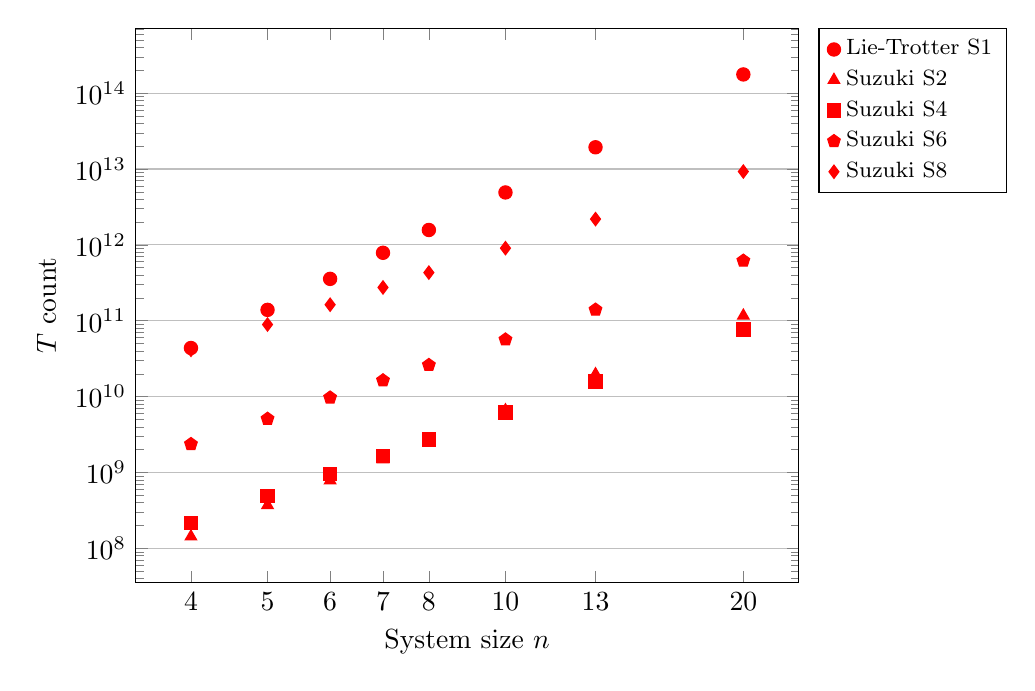
\begin{tikzpicture}
  \begin{loglogaxis}[
    width=10cm,
    xlabel={System size $n$},
    ylabel={$T$ count},
    xtick={4,5,6,7,8,10,13,20},
    xticklabels={4,5,6,7,8,10,13,20},
    ymajorgrids=true,
    legend pos=outer north east,
    legend cell align=left,
    legend style={font=\footnotesize},
  ]
    \addplot[only marks, red, mark=*, mark size=2.4pt, mark options={solid, fill=red}] coordinates {
      (4,43734676060)
      (5,139176030720)
      (6,356460430608)
      (7,786532978980)
      (8,1571954286032)
      (10,4909434449784)
      (13,19343375781604)
      (20,176419535146312)
    };
    \addlegendentry{Lie-Trotter S1}
    \addplot[only marks, red, mark=triangle*, mark size=2.4pt, mark options={solid, fill=red}] coordinates {
      (4,142900064)
      (5,369887232)
      (6,783557726)
      (7,1482803784)
      (8,2587232772)
      (10,6588595800)
      (13,19714975684)
      (20,116606541324)
    };
    \addlegendentry{Suzuki S2}
    \addplot[only marks, red, mark=square*, mark size=2.4pt, mark options={solid, fill=red}] coordinates {
      (4,217129014)
      (5,490265142)
      (6,947562244)
      (7,1660256568)
      (8,2726214260)
      (10,6171351168)
      (13,15873261390)
      (20,76280562330)
    };
    \addlegendentry{Suzuki S4}
    \addplot[only marks, red, mark=pentagon*, mark size=2.4pt, mark options={solid, fill=red}] coordinates {
      (4,2367809968)
      (5,5097618340)
      (6,9714995620)
      (7,16373298184)
      (8,26078648328)
      (10,56517973560)
      (13,139918929000)
      (20,618368280168)
    };
    \addlegendentry{Suzuki S6}
    \addplot[only marks, red, mark=diamond*, mark size=2.4pt, mark options={solid, fill=red}] coordinates {
      (4,41351550240)
      (5,89126606142)
      (6,162780181776)
      (7,274661490840)
      (8,431167981430)
      (10,904986121032)
      (13,2187588939552)
      (20,9258138748774)
    };
    \addlegendentry{Suzuki S8}
  \end{loglogaxis}
\end{tikzpicture}

\clearpage

\section*{\texttt{t/A-min-by-order.tex}}
Suzuki formulas of each order, r from: Minimised bound\par\medskip
% Generated by plsimcount.pffigure -- do not edit; regenerate instead.
% figure: A-min-by-order -- Suzuki formulas of each order, r from: Minimised bound
% source: results/np-main/seed1/results.json
% metric=t gatebase=ct merged
% seed=1 t=n template=simcount synth=pygridsynth
% git_commit=01d3c275ceae2840002bd1aaea68f59b987c4975 git_dirty=False
% source_sha256=0dd1c9775f148df550d3d3f68cfeee1d2d060b7913324535bbf1533b52b4d2c2
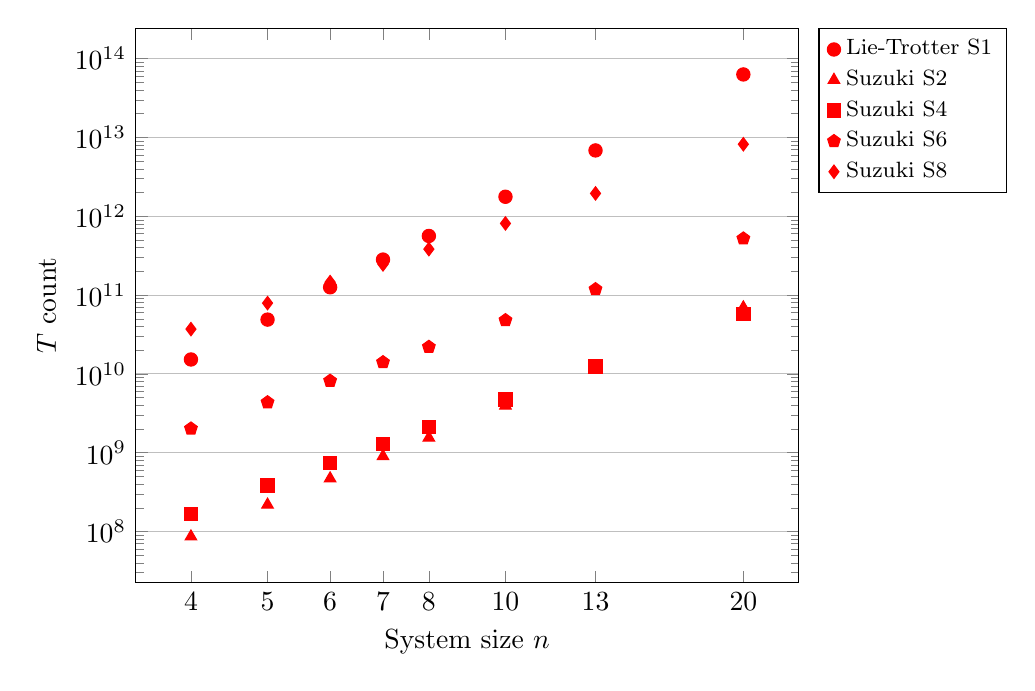
\begin{tikzpicture}
  \begin{loglogaxis}[
    width=10cm,
    xlabel={System size $n$},
    ylabel={$T$ count},
    xtick={4,5,6,7,8,10,13,20},
    xticklabels={4,5,6,7,8,10,13,20},
    ymajorgrids=true,
    legend pos=outer north east,
    legend cell align=left,
    legend style={font=\footnotesize},
  ]
    \addplot[only marks, red, mark=*, mark size=2.4pt, mark options={solid, fill=red}] coordinates {
      (4,15253623168)
      (5,48880244400)
      (6,125660596320)
      (7,282127823712)
      (8,562562122752)
      (10,1768962211200)
      (13,6845505543240)
      (20,63037459699200)
    };
    \addlegendentry{Lie-Trotter S1}
    \addplot[only marks, red, mark=triangle*, mark size=2.4pt, mark options={solid, fill=red}] coordinates {
      (4,86298624)
      (5,218804960)
      (6,470742840)
      (7,901050280)
      (8,1549621936)
      (10,3953322156)
      (13,11725165980)
      (20,69608829112)
    };
    \addlegendentry{Suzuki S2}
    \addplot[only marks, red, mark=square*, mark size=2.4pt, mark options={solid, fill=red}] coordinates {
      (4,167581482)
      (5,382321536)
      (6,735212988)
      (7,1299472296)
      (8,2117499576)
      (10,4749058800)
      (13,12395182464)
      (20,57627905750)
    };
    \addlegendentry{Suzuki S4}
    \addplot[only marks, red, mark=pentagon*, mark size=2.4pt, mark options={solid, fill=red}] coordinates {
      (4,2024782542)
      (5,4360753356)
      (6,8172748976)
      (7,14055074646)
      (8,22006049912)
      (10,48017099500)
      (13,118696724096)
      (20,521672145806)
    };
    \addlegendentry{Suzuki S6}
    \addplot[only marks, red, mark=diamond*, mark size=2.4pt, mark options={solid, fill=red}] coordinates {
      (4,37023325728)
      (5,79151533952)
      (6,146176022952)
      (7,245258541836)
      (8,382948701696)
      (10,811163790000)
      (13,1950511504920)
      (20,8207330049928)
    };
    \addlegendentry{Suzuki S8}
  \end{loglogaxis}
\end{tikzpicture}

\clearpage

\section*{\texttt{t/A-com-by-order.tex}}
Suzuki formulas of each order, r from: Commutator bound (2018)\par\medskip
% Generated by plsimcount.pffigure -- do not edit; regenerate instead.
% figure: A-com-by-order -- Suzuki formulas of each order, r from: Commutator bound (2018)
% source: results/np-main/seed1/results.json
% metric=t gatebase=ct merged
% seed=1 t=n template=simcount synth=pygridsynth
% git_commit=01d3c275ceae2840002bd1aaea68f59b987c4975 git_dirty=False
% source_sha256=0dd1c9775f148df550d3d3f68cfeee1d2d060b7913324535bbf1533b52b4d2c2
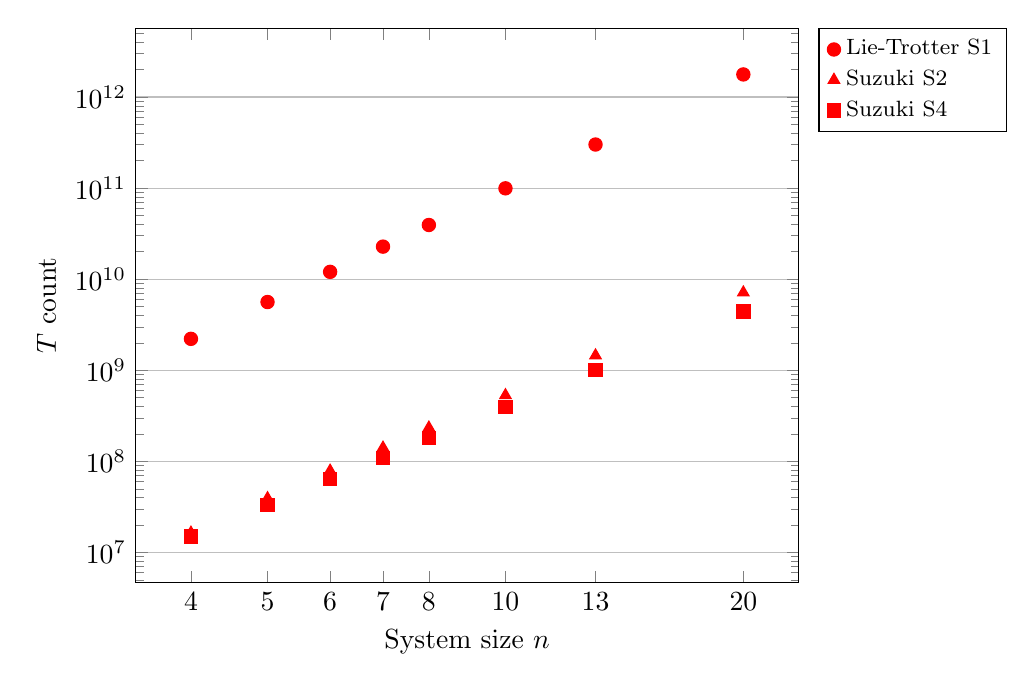
\begin{tikzpicture}
  \begin{loglogaxis}[
    width=10cm,
    xlabel={System size $n$},
    ylabel={$T$ count},
    xtick={4,5,6,7,8,10,13,20},
    xticklabels={4,5,6,7,8,10,13,20},
    ymajorgrids=true,
    legend pos=outer north east,
    legend cell align=left,
    legend style={font=\footnotesize},
  ]
    \addplot[only marks, red, mark=*, mark size=2.4pt, mark options={solid, fill=red}] coordinates {
      (4,2214637010)
      (5,5615599682)
      (6,12036804346)
      (7,22777630240)
      (8,39366761492)
      (10,99370601712)
      (13,300757437828)
      (20,1767868545168)
    };
    \addlegendentry{Lie-Trotter S1}
    \addplot[only marks, red, mark=triangle*, mark size=2.4pt, mark options={solid, fill=red}] coordinates {
      (4,16448124)
      (5,39306456)
      (6,78821280)
      (7,140949800)
      (8,234043080)
      (10,531045440)
      (13,1451578560)
      (20,7125229868)
    };
    \addlegendentry{Suzuki S2}
    \addplot[only marks, red, mark=square*, mark size=2.4pt, mark options={solid, fill=red}] coordinates {
      (4,14953600)
      (5,33012860)
      (6,64032276)
      (7,109665556)
      (8,179648608)
      (10,396099620)
      (13,1006846032)
      (20,4428589536)
    };
    \addlegendentry{Suzuki S4}
  \end{loglogaxis}
\end{tikzpicture}

\clearpage

\section*{\texttt{t/A-emp-by-order.tex}}
Suzuki formulas of each order, r from: Empirical fit (2018)\par\medskip
% Generated by pysimcount.pffigure -- do not edit; regenerate instead.
% figure: A-emp-by-order -- Suzuki formulas of each order, r from: Empirical fit (2018)
% source: results/np-main/seed1/results.json
% metric=t gatebase=ct merged
% seed=1 t=n template=simcount synth=pygridsynth
% git_commit=01d3c275ceae2840002bd1aaea68f59b987c4975 git_dirty=False
% source_sha256=0dd1c9775f148df550d3d3f68cfeee1d2d060b7913324535bbf1533b52b4d2c2
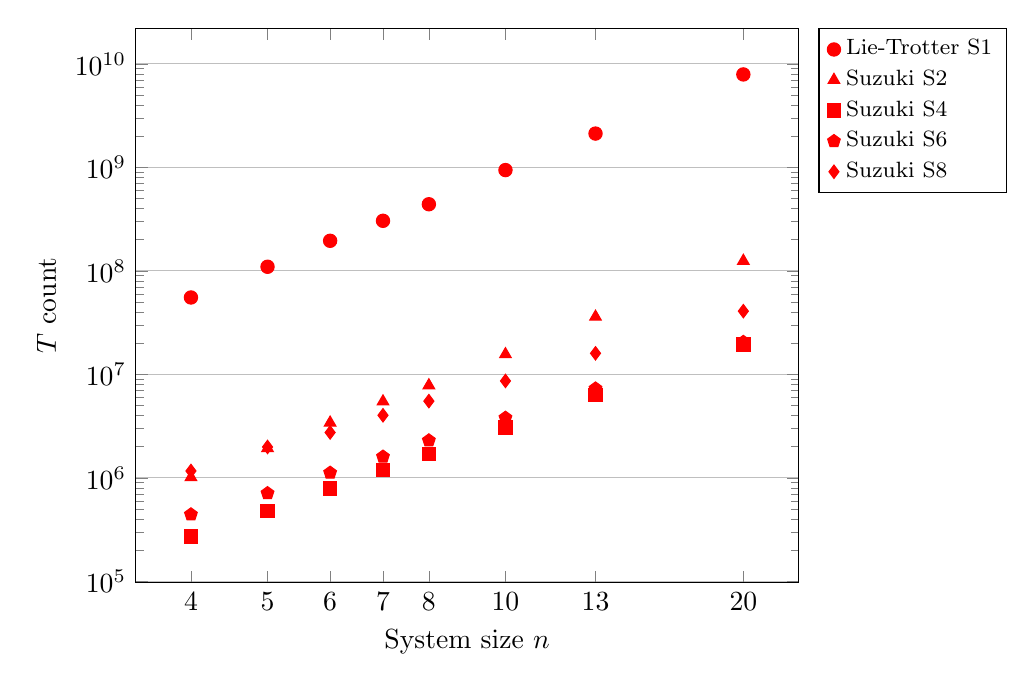
\begin{tikzpicture}
  \begin{loglogaxis}[
    width=10cm,
    xlabel={System size $n$},
    ylabel={$T$ count},
    xtick={4,5,6,7,8,10,13,20},
    xticklabels={4,5,6,7,8,10,13,20},
    ymajorgrids=true,
    legend pos=outer north east,
    legend cell align=left,
    legend style={font=\footnotesize},
  ]
    \addplot[only marks, red, mark=*, mark size=2.4pt, mark options={solid, fill=red}] coordinates {
      (4,55338176)
      (5,109611660)
      (6,195319278)
      (7,304797840)
      (8,440692360)
      (10,942510000)
      (13,2123943682)
      (20,7918571028)
    };
    \addlegendentry{Lie-Trotter S1}
    \addplot[only marks, red, mark=triangle*, mark size=2.4pt, mark options={solid, fill=red}] coordinates {
      (4,1012782)
      (5,1929754)
      (6,3409920)
      (7,5463920)
      (8,7821000)
      (10,15625418)
      (13,35990730)
      (20,124776288)
    };
    \addlegendentry{Suzuki S2}
    \addplot[only marks, red, mark=square*, mark size=2.4pt, mark options={solid, fill=red}] coordinates {
      (4,270410)
      (5,480600)
      (6,790152)
      (7,1183728)
      (8,1698264)
      (10,3073420)
      (13,6353392)
      (20,19508350)
    };
    \addlegendentry{Suzuki S4}
    \addplot[only marks, red, mark=pentagon*, mark size=2.4pt, mark options={solid, fill=red}] coordinates {
      (4,442560)
      (5,709620)
      (6,1118188)
      (7,1599282)
      (8,2296392)
      (10,3800566)
      (13,7287904)
      (20,20534332)
    };
    \addlegendentry{Suzuki S6}
    \addplot[only marks, red, mark=diamond*, mark size=2.4pt, mark options={solid, fill=red}] coordinates {
      (4,1164552)
      (5,1986752)
      (6,2741688)
      (7,4023074)
      (8,5513378)
      (10,8632000)
      (13,15967908)
      (20,40825400)
    };
    \addlegendentry{Suzuki S8}
  \end{loglogaxis}
\end{tikzpicture}

\clearpage

\section*{\texttt{t/A-tte-by-order.tex}}
Suzuki formulas of each order, r from: Commutator bound (2021)\par\medskip
% Generated by pysimcount.pffigure -- do not edit; regenerate instead.
% figure: A-tte-by-order -- Suzuki formulas of each order, r from: Commutator bound (2021)
% source: results/np-main/seed1/results.json
% metric=t gatebase=ct merged
% seed=1 t=n template=simcount synth=pygridsynth
% git_commit=01d3c275ceae2840002bd1aaea68f59b987c4975 git_dirty=False
% source_sha256=0dd1c9775f148df550d3d3f68cfeee1d2d060b7913324535bbf1533b52b4d2c2
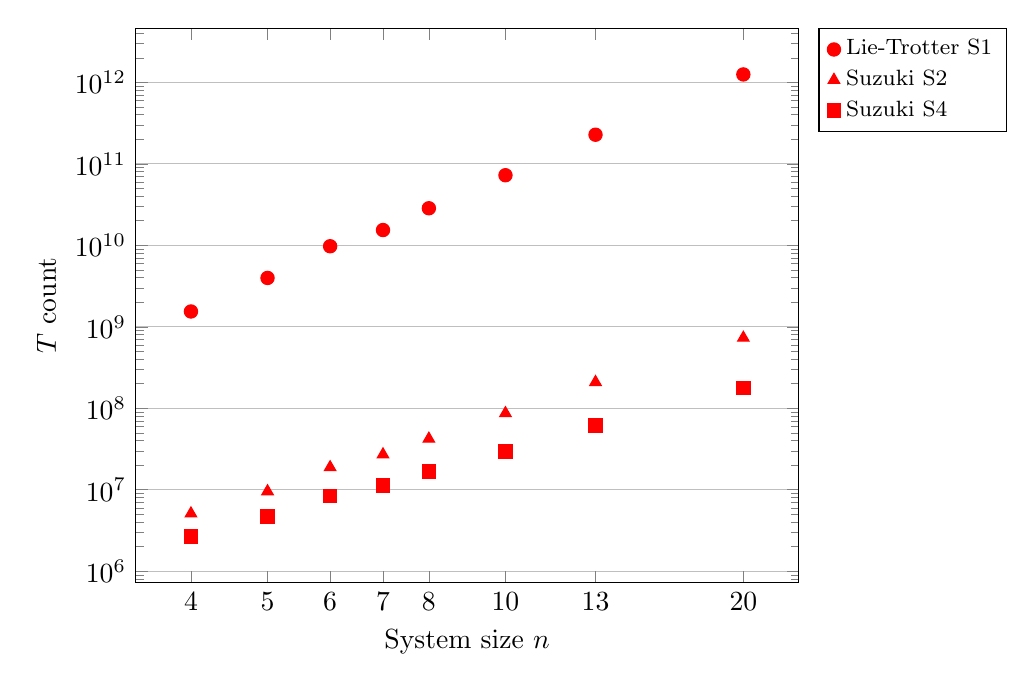
\begin{tikzpicture}
  \begin{loglogaxis}[
    width=10cm,
    xlabel={System size $n$},
    ylabel={$T$ count},
    xtick={4,5,6,7,8,10,13,20},
    xticklabels={4,5,6,7,8,10,13,20},
    ymajorgrids=true,
    legend pos=outer north east,
    legend cell align=left,
    legend style={font=\footnotesize},
  ]
    \addplot[only marks, red, mark=*, mark size=2.4pt, mark options={solid, fill=red}] coordinates {
      (4,1541003046)
      (5,3975916568)
      (6,9734529750)
      (7,15401664696)
      (8,28490016480)
      (10,72418196796)
      (13,227624550646)
      (20,1250277877772)
    };
    \addlegendentry{Lie-Trotter S1}
    \addplot[only marks, red, mark=triangle*, mark size=2.4pt, mark options={solid, fill=red}] coordinates {
      (4,5096824)
      (5,9543744)
      (6,18827328)
      (7,27039896)
      (8,42148120)
      (10,86752020)
      (13,209010544)
      (20,731040960)
    };
    \addlegendentry{Suzuki S2}
    \addplot[only marks, red, mark=square*, mark size=2.4pt, mark options={solid, fill=red}] coordinates {
      (4,2661098)
      (5,4701024)
      (6,8314572)
      (7,11267100)
      (8,16796502)
      (10,29484208)
      (13,61637022)
      (20,178374976)
    };
    \addlegendentry{Suzuki S4}
  \end{loglogaxis}
\end{tikzpicture}

\clearpage

\section*{\texttt{t/A-measured-by-order.tex}}
Suzuki formulas of each order, r from: Measured $r$\par\medskip
% Generated by pysimcount.pffigure -- do not edit; regenerate instead.
% figure: A-measured-by-order -- Suzuki formulas of each order, r from: Measured $r$
% source: results/np-main/seed1/results.json
% metric=t gatebase=ct merged
% seed=1 t=n template=simcount synth=pygridsynth
% git_commit=01d3c275ceae2840002bd1aaea68f59b987c4975 git_dirty=False
% source_sha256=0dd1c9775f148df550d3d3f68cfeee1d2d060b7913324535bbf1533b52b4d2c2
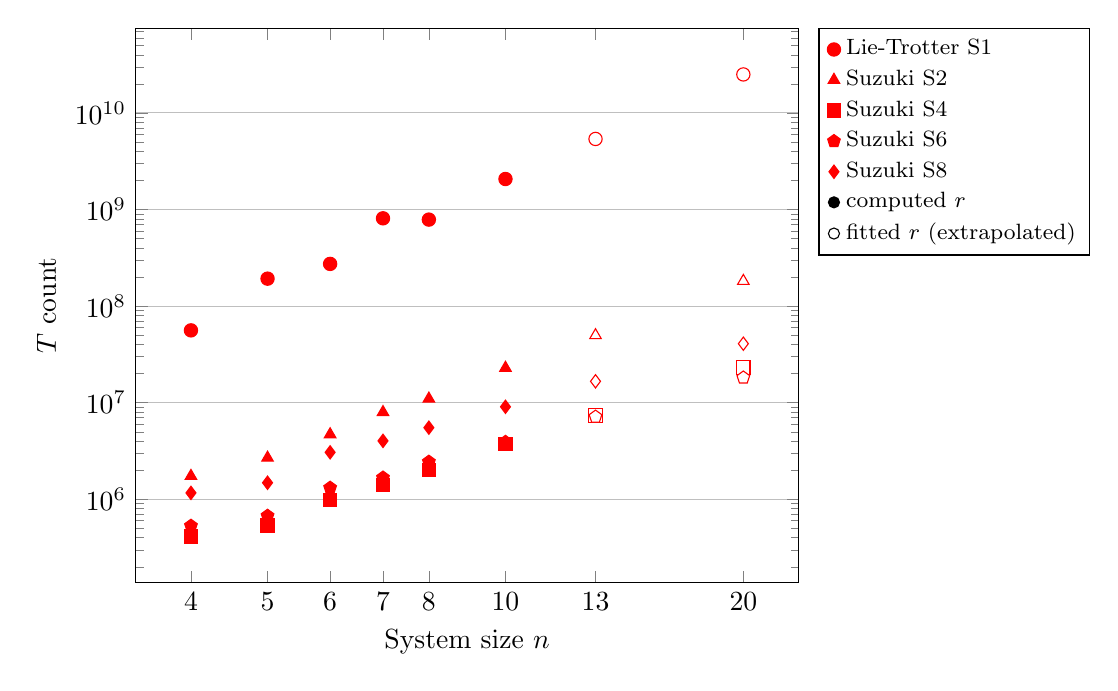
\begin{tikzpicture}
  \begin{loglogaxis}[
    width=10cm,
    xlabel={System size $n$},
    ylabel={$T$ count},
    xtick={4,5,6,7,8,10,13,20},
    xticklabels={4,5,6,7,8,10,13,20},
    ymajorgrids=true,
    legend pos=outer north east,
    legend cell align=left,
    legend style={font=\footnotesize},
  ]
    \addplot[only marks, red, mark=*, mark size=2.4pt, mark options={solid, fill=red}] coordinates {
      (4,56093184)
      (5,192444928)
      (6,273474232)
      (7,810858048)
      (8,786590496)
      (10,2070142340)
    };
    \addlegendentry{Lie-Trotter S1}
    % r from power-law fit (extrapolation); one legend entry per series
    \addplot[only marks, red, mark=*, mark size=2.4pt, mark options={solid, fill=white}, forget plot] coordinates {
      (13,5379060774)
      (20,25039558558)
    };
    \addplot[only marks, red, mark=triangle*, mark size=2.4pt, mark options={solid, fill=red}] coordinates {
      (4,1739724)
      (5,2687776)
      (6,4698130)
      (7,7969260)
      (8,10989048)
      (10,22900530)
    };
    \addlegendentry{Suzuki S2}
    % r from power-law fit (extrapolation); one legend entry per series
    \addplot[only marks, red, mark=triangle*, mark size=2.4pt, mark options={solid, fill=white}, forget plot] coordinates {
      (13,49822284)
      (20,181860528)
    };
    \addplot[only marks, red, mark=square*, mark size=2.4pt, mark options={solid, fill=red}] coordinates {
      (4,410856)
      (5,534710)
      (6,987026)
      (7,1404340)
      (8,2020560)
      (10,3710728)
    };
    \addlegendentry{Suzuki S4}
    % r from power-law fit (extrapolation); one legend entry per series
    \addplot[only marks, red, mark=square*, mark size=2.4pt, mark options={solid, fill=white}, forget plot] coordinates {
      (13,7377150)
      (20,23100384)
    };
    \addplot[only marks, red, mark=pentagon*, mark size=2.4pt, mark options={solid, fill=red}] coordinates {
      (4,530964)
      (5,673708)
      (6,1314412)
      (7,1673760)
      (8,2443080)
      (10,3919244)
    };
    \addlegendentry{Suzuki S6}
    % r from power-law fit (extrapolation); one legend entry per series
    \addplot[only marks, red, mark=pentagon*, mark size=2.4pt, mark options={solid, fill=white}, forget plot] coordinates {
      (13,7156932)
      (20,18178252)
    };
    \addplot[only marks, red, mark=diamond*, mark size=2.4pt, mark options={solid, fill=red}] coordinates {
      (4,1164552)
      (5,1483068)
      (6,3062680)
      (7,4023074)
      (8,5513378)
      (10,9073036)
    };
    \addlegendentry{Suzuki S8}
    % r from power-law fit (extrapolation); one legend entry per series
    \addplot[only marks, red, mark=diamond*, mark size=2.4pt, mark options={solid, fill=white}, forget plot] coordinates {
      (13,16651540)
      (20,40825400)
    };
    \addlegendimage{only marks, black, mark=*, mark options={fill=black}}
    \addlegendentry{computed $r$}
    \addlegendimage{only marks, black, mark=*, mark options={fill=white}}
    \addlegendentry{fitted $r$ (extrapolated)}
  \end{loglogaxis}
\end{tikzpicture}

\clearpage

\section*{\texttt{t/B-order4-by-formula.tex}}
Every order-4 formula at measured r\par\medskip
% Generated by pysimcount.pffigure -- do not edit; regenerate instead.
% figure: B-order4-by-formula -- Every order-4 formula at measured r
% source: results/np-main/seed1/results.json
% metric=t gatebase=ct merged
% seed=1 t=n template=simcount synth=pygridsynth
% git_commit=01d3c275ceae2840002bd1aaea68f59b987c4975 git_dirty=False
% source_sha256=0dd1c9775f148df550d3d3f68cfeee1d2d060b7913324535bbf1533b52b4d2c2
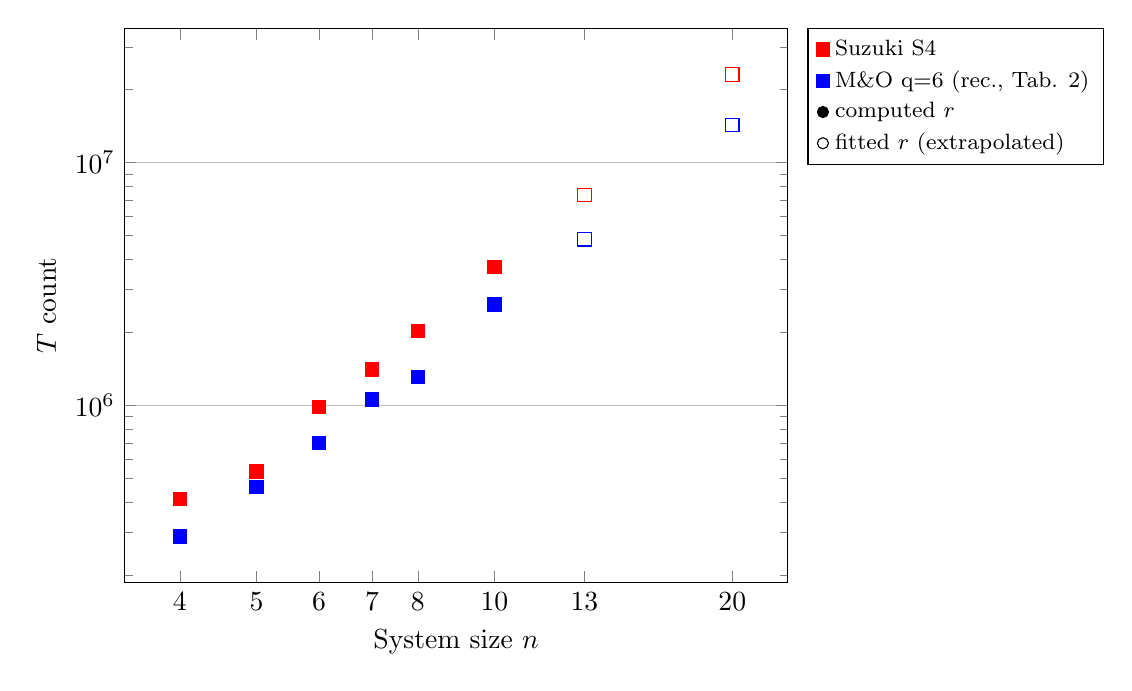
\begin{tikzpicture}
  \begin{loglogaxis}[
    width=10cm,
    xlabel={System size $n$},
    ylabel={$T$ count},
    xtick={4,5,6,7,8,10,13,20},
    xticklabels={4,5,6,7,8,10,13,20},
    ymajorgrids=true,
    legend pos=outer north east,
    legend cell align=left,
    legend style={font=\footnotesize},
  ]
    \addplot[only marks, red, mark=square*, mark size=2.4pt, mark options={solid, fill=red}] coordinates {
      (4,410856)
      (5,534710)
      (6,987026)
      (7,1404340)
      (8,2020560)
      (10,3710728)
    };
    \addlegendentry{Suzuki S4}
    % r from power-law fit (extrapolation); one legend entry per series
    \addplot[only marks, red, mark=square*, mark size=2.4pt, mark options={solid, fill=white}, forget plot] coordinates {
      (13,7377150)
      (20,23100384)
    };
    \addplot[only marks, blue, mark=square*, mark size=2.4pt, mark options={solid, fill=blue}] coordinates {
      (4,288000)
      (5,461360)
      (6,701600)
      (7,1058148)
      (8,1310224)
      (10,2607488)
    };
    \addlegendentry{M\&O q=6 (rec., Tab. 2)}
    % r from power-law fit (extrapolation); one legend entry per series
    \addplot[only marks, blue, mark=square*, mark size=2.4pt, mark options={solid, fill=white}, forget plot] coordinates {
      (13,4833430)
      (20,14317248)
    };
    \addlegendimage{only marks, black, mark=*, mark options={fill=black}}
    \addlegendentry{computed $r$}
    \addlegendimage{only marks, black, mark=*, mark options={fill=white}}
    \addlegendentry{fitted $r$ (extrapolated)}
  \end{loglogaxis}
\end{tikzpicture}

\clearpage

\section*{\texttt{t/B-order6-by-formula.tex}}
Every order-6 formula at measured r\par\medskip
% Generated by plsimcount.pffigure -- do not edit; regenerate instead.
% figure: B-order6-by-formula -- Every order-6 formula at measured r
% source: results/np-main/seed1/results.json
% metric=t gatebase=ct merged
% seed=1 t=n template=simcount synth=pygridsynth
% git_commit=01d3c275ceae2840002bd1aaea68f59b987c4975 git_dirty=False
% source_sha256=0dd1c9775f148df550d3d3f68cfeee1d2d060b7913324535bbf1533b52b4d2c2
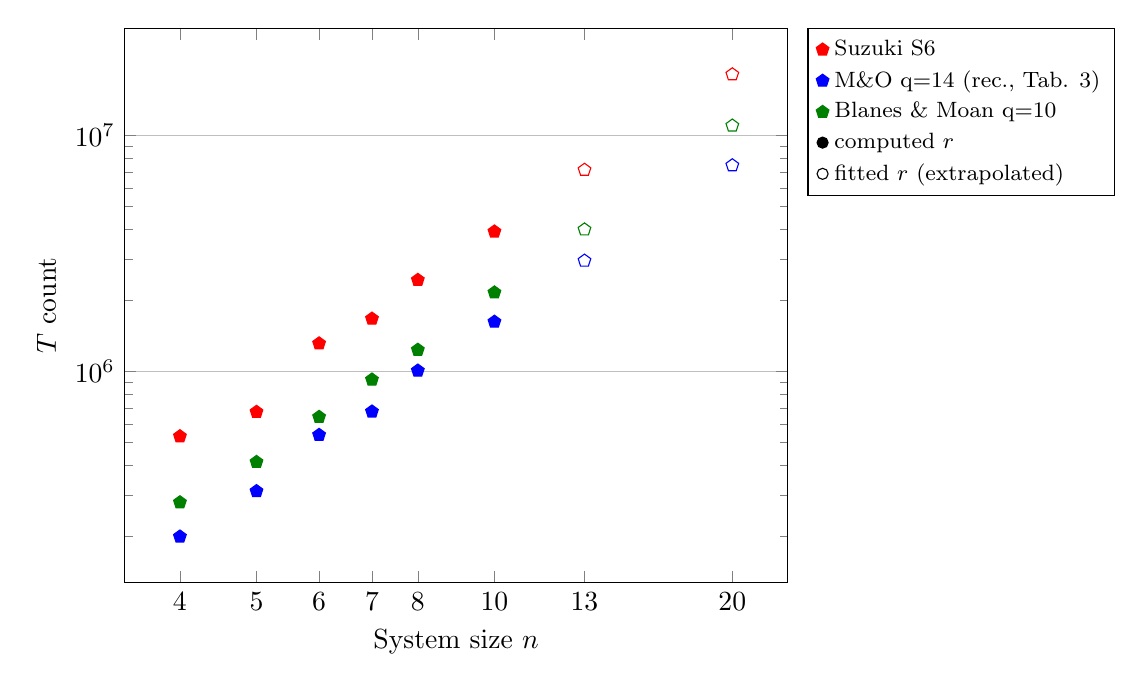
\begin{tikzpicture}
  \begin{loglogaxis}[
    width=10cm,
    xlabel={System size $n$},
    ylabel={$T$ count},
    xtick={4,5,6,7,8,10,13,20},
    xticklabels={4,5,6,7,8,10,13,20},
    ymajorgrids=true,
    legend pos=outer north east,
    legend cell align=left,
    legend style={font=\footnotesize},
  ]
    \addplot[only marks, red, mark=pentagon*, mark size=2.4pt, mark options={solid, fill=red}] coordinates {
      (4,530964)
      (5,673708)
      (6,1314412)
      (7,1673760)
      (8,2443080)
      (10,3919244)
    };
    \addlegendentry{Suzuki S6}
    % r from power-law fit (extrapolation); one legend entry per series
    \addplot[only marks, red, mark=pentagon*, mark size=2.4pt, mark options={solid, fill=white}, forget plot] coordinates {
      (13,7156932)
      (20,18178252)
    };
    \addplot[only marks, blue, mark=pentagon*, mark size=2.4pt, mark options={solid, fill=blue}] coordinates {
      (4,199480)
      (5,310776)
      (6,538016)
      (7,676044)
      (8,1008044)
      (10,1624000)
    };
    \addlegendentry{M\&O q=14 (rec., Tab. 3)}
    % r from power-law fit (extrapolation); one legend entry per series
    \addplot[only marks, blue, mark=pentagon*, mark size=2.4pt, mark options={solid, fill=white}, forget plot] coordinates {
      (13,2948400)
      (20,7479184)
    };
    \addplot[only marks, green!50!black, mark=pentagon*, mark size=2.4pt, mark options={solid, fill=green!50!black}] coordinates {
      (4,278692)
      (5,413072)
      (6,641424)
      (7,923508)
      (8,1235364)
      (10,2161552)
    };
    \addlegendentry{Blanes \& Moan q=10}
    % r from power-law fit (extrapolation); one legend entry per series
    \addplot[only marks, green!50!black, mark=pentagon*, mark size=2.4pt, mark options={solid, fill=white}, forget plot] coordinates {
      (13,3998064)
      (20,11023104)
    };
    \addlegendimage{only marks, black, mark=*, mark options={fill=black}}
    \addlegendentry{computed $r$}
    \addlegendimage{only marks, black, mark=*, mark options={fill=white}}
    \addlegendentry{fitted $r$ (extrapolated)}
  \end{loglogaxis}
\end{tikzpicture}

\clearpage

\section*{\texttt{t/B-order8-by-formula.tex}}
Every order-8 formula at measured r\par\medskip
% Generated by pysimcount.pffigure -- do not edit; regenerate instead.
% figure: B-order8-by-formula -- Every order-8 formula at measured r
% source: results/np-main/seed1/results.json
% metric=t gatebase=ct merged
% seed=1 t=n template=simcount synth=pygridsynth
% git_commit=01d3c275ceae2840002bd1aaea68f59b987c4975 git_dirty=False
% source_sha256=0dd1c9775f148df550d3d3f68cfeee1d2d060b7913324535bbf1533b52b4d2c2
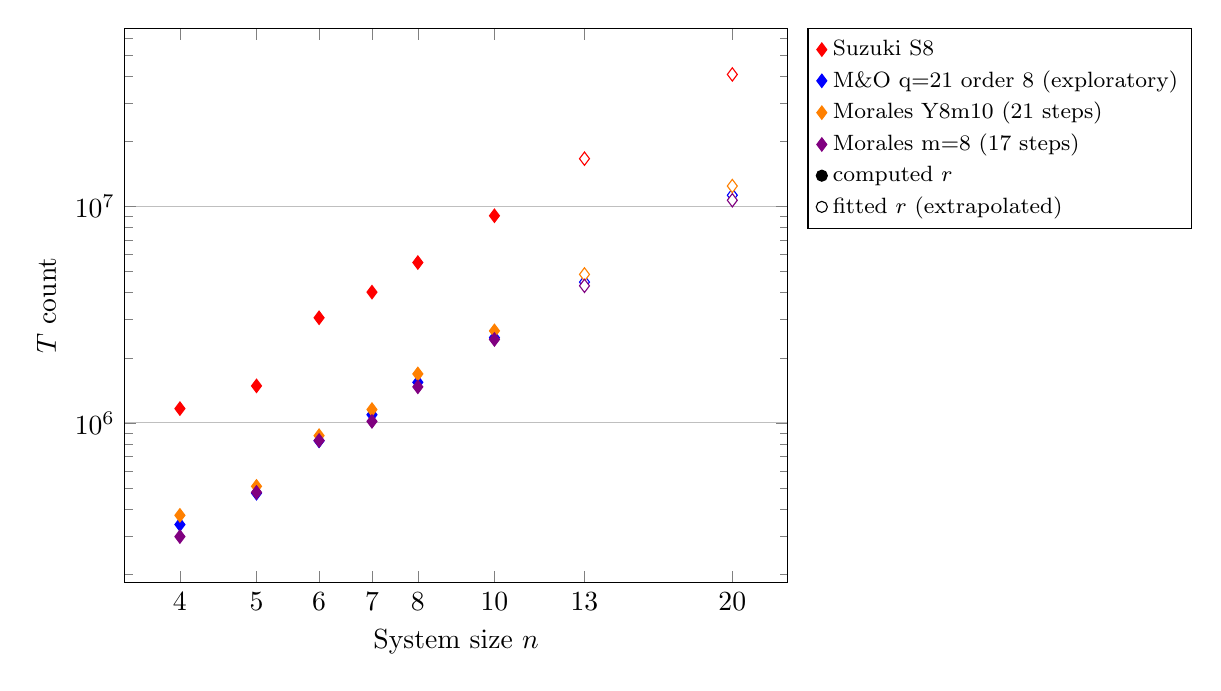
\begin{tikzpicture}
  \begin{loglogaxis}[
    width=10cm,
    xlabel={System size $n$},
    ylabel={$T$ count},
    xtick={4,5,6,7,8,10,13,20},
    xticklabels={4,5,6,7,8,10,13,20},
    ymajorgrids=true,
    legend pos=outer north east,
    legend cell align=left,
    legend style={font=\footnotesize},
  ]
    \addplot[only marks, red, mark=diamond*, mark size=2.4pt, mark options={solid, fill=red}] coordinates {
      (4,1164552)
      (5,1483068)
      (6,3062680)
      (7,4023074)
      (8,5513378)
      (10,9073036)
    };
    \addlegendentry{Suzuki S8}
    % r from power-law fit (extrapolation); one legend entry per series
    \addplot[only marks, red, mark=diamond*, mark size=2.4pt, mark options={solid, fill=white}, forget plot] coordinates {
      (13,16651540)
      (20,40825400)
    };
    \addplot[only marks, blue, mark=diamond*, mark size=2.4pt, mark options={solid, fill=blue}] coordinates {
      (4,339064)
      (5,473304)
      (6,826404)
      (7,1090942)
      (8,1540862)
      (10,2478630)
    };
    \addlegendentry{M\&O q=21 order 8 (exploratory)}
    % r from power-law fit (extrapolation); one legend entry per series
    \addplot[only marks, blue, mark=diamond*, mark size=2.4pt, mark options={solid, fill=white}, forget plot] coordinates {
      (13,4477512)
      (20,11284878)
    };
    \addplot[only marks, orange, mark=diamond*, mark size=2.4pt, mark options={solid, fill=orange}] coordinates {
      (4,374088)
      (5,509288)
      (6,873540)
      (7,1153080)
      (8,1685200)
      (10,2664264)
    };
    \addlegendentry{Morales Y8m10 (21 steps)}
    % r from power-law fit (extrapolation); one legend entry per series
    \addplot[only marks, orange, mark=diamond*, mark size=2.4pt, mark options={solid, fill=white}, forget plot] coordinates {
      (13,4859064)
      (20,12445250)
    };
    \addplot[only marks, violet, mark=diamond*, mark size=2.4pt, mark options={solid, fill=violet}] coordinates {
      (4,298248)
      (5,477630)
      (6,829500)
      (7,1016752)
      (8,1467828)
      (10,2431170)
    };
    \addlegendentry{Morales m=8 (17 steps)}
    % r from power-law fit (extrapolation); one legend entry per series
    \addplot[only marks, violet, mark=diamond*, mark size=2.4pt, mark options={solid, fill=white}, forget plot] coordinates {
      (13,4303300)
      (20,10697428)
    };
    \addlegendimage{only marks, black, mark=*, mark options={fill=black}}
    \addlegendentry{computed $r$}
    \addlegendimage{only marks, black, mark=*, mark options={fill=white}}
    \addlegendentry{fitted $r$ (extrapolated)}
  \end{loglogaxis}
\end{tikzpicture}

\clearpage

\section*{\texttt{t/B-all-by-formula.tex}}
Every formula at measured r\par\medskip
% Generated by pysimcount.pffigure -- do not edit; regenerate instead.
% figure: B-all-by-formula -- Every formula at measured r
% source: results/np-main/seed1/results.json
% metric=t gatebase=ct merged
% seed=1 t=n template=simcount synth=pygridsynth
% git_commit=01d3c275ceae2840002bd1aaea68f59b987c4975 git_dirty=False
% source_sha256=0dd1c9775f148df550d3d3f68cfeee1d2d060b7913324535bbf1533b52b4d2c2
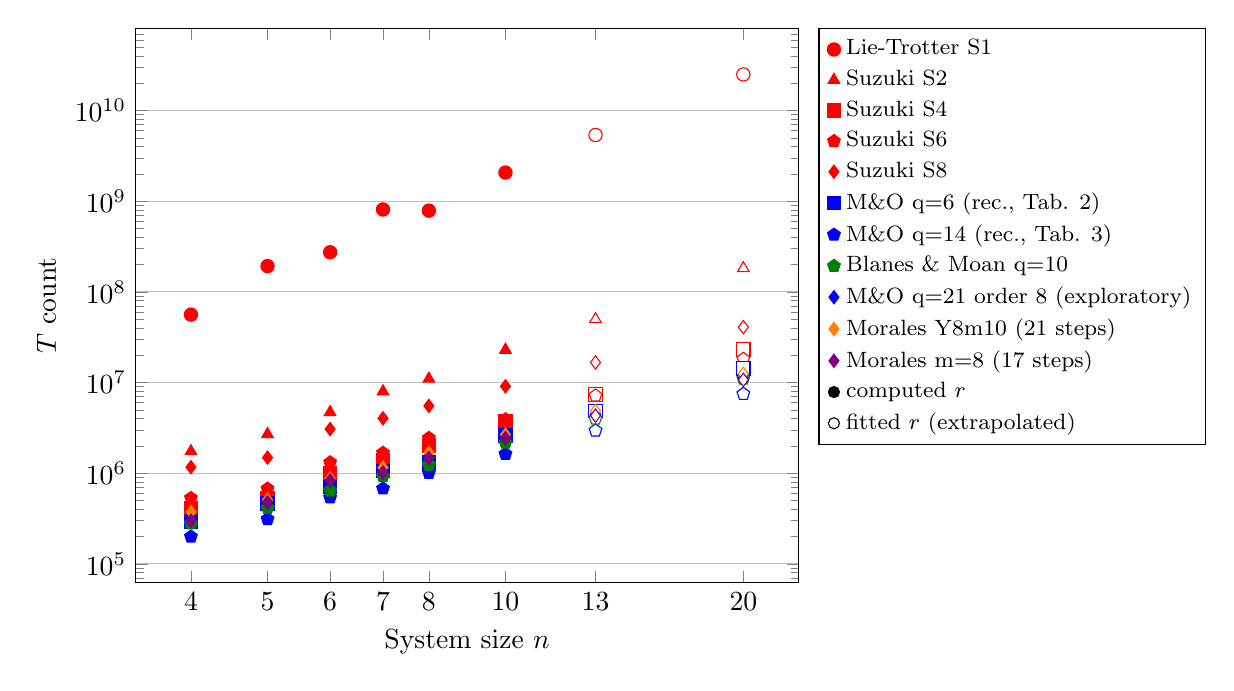
\begin{tikzpicture}
  \begin{loglogaxis}[
    width=10cm,
    xlabel={System size $n$},
    ylabel={$T$ count},
    xtick={4,5,6,7,8,10,13,20},
    xticklabels={4,5,6,7,8,10,13,20},
    ymajorgrids=true,
    legend pos=outer north east,
    legend cell align=left,
    legend style={font=\footnotesize},
  ]
    \addplot[only marks, red, mark=*, mark size=2.4pt, mark options={solid, fill=red}] coordinates {
      (4,56093184)
      (5,192444928)
      (6,273474232)
      (7,810858048)
      (8,786590496)
      (10,2070142340)
    };
    \addlegendentry{Lie-Trotter S1}
    % r from power-law fit (extrapolation); one legend entry per series
    \addplot[only marks, red, mark=*, mark size=2.4pt, mark options={solid, fill=white}, forget plot] coordinates {
      (13,5379060774)
      (20,25039558558)
    };
    \addplot[only marks, red, mark=triangle*, mark size=2.4pt, mark options={solid, fill=red}] coordinates {
      (4,1739724)
      (5,2687776)
      (6,4698130)
      (7,7969260)
      (8,10989048)
      (10,22900530)
    };
    \addlegendentry{Suzuki S2}
    % r from power-law fit (extrapolation); one legend entry per series
    \addplot[only marks, red, mark=triangle*, mark size=2.4pt, mark options={solid, fill=white}, forget plot] coordinates {
      (13,49822284)
      (20,181860528)
    };
    \addplot[only marks, red, mark=square*, mark size=2.4pt, mark options={solid, fill=red}] coordinates {
      (4,410856)
      (5,534710)
      (6,987026)
      (7,1404340)
      (8,2020560)
      (10,3710728)
    };
    \addlegendentry{Suzuki S4}
    % r from power-law fit (extrapolation); one legend entry per series
    \addplot[only marks, red, mark=square*, mark size=2.4pt, mark options={solid, fill=white}, forget plot] coordinates {
      (13,7377150)
      (20,23100384)
    };
    \addplot[only marks, red, mark=pentagon*, mark size=2.4pt, mark options={solid, fill=red}] coordinates {
      (4,530964)
      (5,673708)
      (6,1314412)
      (7,1673760)
      (8,2443080)
      (10,3919244)
    };
    \addlegendentry{Suzuki S6}
    % r from power-law fit (extrapolation); one legend entry per series
    \addplot[only marks, red, mark=pentagon*, mark size=2.4pt, mark options={solid, fill=white}, forget plot] coordinates {
      (13,7156932)
      (20,18178252)
    };
    \addplot[only marks, red, mark=diamond*, mark size=2.4pt, mark options={solid, fill=red}] coordinates {
      (4,1164552)
      (5,1483068)
      (6,3062680)
      (7,4023074)
      (8,5513378)
      (10,9073036)
    };
    \addlegendentry{Suzuki S8}
    % r from power-law fit (extrapolation); one legend entry per series
    \addplot[only marks, red, mark=diamond*, mark size=2.4pt, mark options={solid, fill=white}, forget plot] coordinates {
      (13,16651540)
      (20,40825400)
    };
    \addplot[only marks, blue, mark=square*, mark size=2.4pt, mark options={solid, fill=blue}] coordinates {
      (4,288000)
      (5,461360)
      (6,701600)
      (7,1058148)
      (8,1310224)
      (10,2607488)
    };
    \addlegendentry{M\&O q=6 (rec., Tab. 2)}
    % r from power-law fit (extrapolation); one legend entry per series
    \addplot[only marks, blue, mark=square*, mark size=2.4pt, mark options={solid, fill=white}, forget plot] coordinates {
      (13,4833430)
      (20,14317248)
    };
    \addplot[only marks, blue, mark=pentagon*, mark size=2.4pt, mark options={solid, fill=blue}] coordinates {
      (4,199480)
      (5,310776)
      (6,538016)
      (7,676044)
      (8,1008044)
      (10,1624000)
    };
    \addlegendentry{M\&O q=14 (rec., Tab. 3)}
    % r from power-law fit (extrapolation); one legend entry per series
    \addplot[only marks, blue, mark=pentagon*, mark size=2.4pt, mark options={solid, fill=white}, forget plot] coordinates {
      (13,2948400)
      (20,7479184)
    };
    \addplot[only marks, green!50!black, mark=pentagon*, mark size=2.4pt, mark options={solid, fill=green!50!black}] coordinates {
      (4,278692)
      (5,413072)
      (6,641424)
      (7,923508)
      (8,1235364)
      (10,2161552)
    };
    \addlegendentry{Blanes \& Moan q=10}
    % r from power-law fit (extrapolation); one legend entry per series
    \addplot[only marks, green!50!black, mark=pentagon*, mark size=2.4pt, mark options={solid, fill=white}, forget plot] coordinates {
      (13,3998064)
      (20,11023104)
    };
    \addplot[only marks, blue, mark=diamond*, mark size=2.4pt, mark options={solid, fill=blue}] coordinates {
      (4,339064)
      (5,473304)
      (6,826404)
      (7,1090942)
      (8,1540862)
      (10,2478630)
    };
    \addlegendentry{M\&O q=21 order 8 (exploratory)}
    % r from power-law fit (extrapolation); one legend entry per series
    \addplot[only marks, blue, mark=diamond*, mark size=2.4pt, mark options={solid, fill=white}, forget plot] coordinates {
      (13,4477512)
      (20,11284878)
    };
    \addplot[only marks, orange, mark=diamond*, mark size=2.4pt, mark options={solid, fill=orange}] coordinates {
      (4,374088)
      (5,509288)
      (6,873540)
      (7,1153080)
      (8,1685200)
      (10,2664264)
    };
    \addlegendentry{Morales Y8m10 (21 steps)}
    % r from power-law fit (extrapolation); one legend entry per series
    \addplot[only marks, orange, mark=diamond*, mark size=2.4pt, mark options={solid, fill=white}, forget plot] coordinates {
      (13,4859064)
      (20,12445250)
    };
    \addplot[only marks, violet, mark=diamond*, mark size=2.4pt, mark options={solid, fill=violet}] coordinates {
      (4,298248)
      (5,477630)
      (6,829500)
      (7,1016752)
      (8,1467828)
      (10,2431170)
    };
    \addlegendentry{Morales m=8 (17 steps)}
    % r from power-law fit (extrapolation); one legend entry per series
    \addplot[only marks, violet, mark=diamond*, mark size=2.4pt, mark options={solid, fill=white}, forget plot] coordinates {
      (13,4303300)
      (20,10697428)
    };
    \addlegendimage{only marks, black, mark=*, mark options={fill=black}}
    \addlegendentry{computed $r$}
    \addlegendimage{only marks, black, mark=*, mark options={fill=white}}
    \addlegendentry{fitted $r$ (extrapolated)}
  \end{loglogaxis}
\end{tikzpicture}

\clearpage

\section*{\texttt{t/C-lie-trotter-by-bound.tex}}
Lie-Trotter S1: r from each bound and measured\par\medskip
% Generated by plsimcount.pffigure -- do not edit; regenerate instead.
% figure: C-lie-trotter-by-bound -- Lie-Trotter S1: r from each bound and measured
% source: results/np-main/seed1/results.json
% metric=t gatebase=ct merged
% seed=1 t=n template=simcount synth=pygridsynth
% git_commit=01d3c275ceae2840002bd1aaea68f59b987c4975 git_dirty=False
% source_sha256=0dd1c9775f148df550d3d3f68cfeee1d2d060b7913324535bbf1533b52b4d2c2
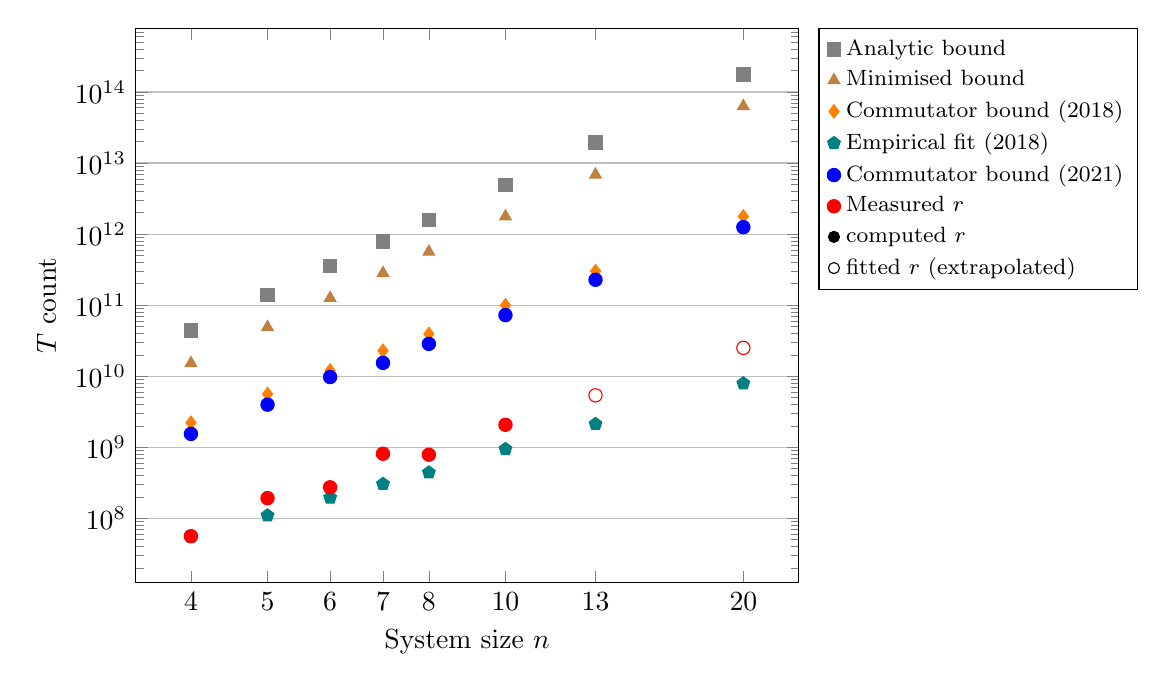
\begin{tikzpicture}
  \begin{loglogaxis}[
    width=10cm,
    xlabel={System size $n$},
    ylabel={$T$ count},
    xtick={4,5,6,7,8,10,13,20},
    xticklabels={4,5,6,7,8,10,13,20},
    ymajorgrids=true,
    legend pos=outer north east,
    legend cell align=left,
    legend style={font=\footnotesize},
  ]
    \addplot[only marks, gray, mark=square*, mark size=2.4pt, mark options={solid, fill=gray}] coordinates {
      (4,43734676060)
      (5,139176030720)
      (6,356460430608)
      (7,786532978980)
      (8,1571954286032)
      (10,4909434449784)
      (13,19343375781604)
      (20,176419535146312)
    };
    \addlegendentry{Analytic bound}
    \addplot[only marks, brown, mark=triangle*, mark size=2.4pt, mark options={solid, fill=brown}] coordinates {
      (4,15253623168)
      (5,48880244400)
      (6,125660596320)
      (7,282127823712)
      (8,562562122752)
      (10,1768962211200)
      (13,6845505543240)
      (20,63037459699200)
    };
    \addlegendentry{Minimised bound}
    \addplot[only marks, orange, mark=diamond*, mark size=2.4pt, mark options={solid, fill=orange}] coordinates {
      (4,2214637010)
      (5,5615599682)
      (6,12036804346)
      (7,22777630240)
      (8,39366761492)
      (10,99370601712)
      (13,300757437828)
      (20,1767868545168)
    };
    \addlegendentry{Commutator bound (2018)}
    \addplot[only marks, teal, mark=pentagon*, mark size=2.4pt, mark options={solid, fill=teal}] coordinates {
      (4,55338176)
      (5,109611660)
      (6,195319278)
      (7,304797840)
      (8,440692360)
      (10,942510000)
      (13,2123943682)
      (20,7918571028)
    };
    \addlegendentry{Empirical fit (2018)}
    \addplot[only marks, blue, mark=oplus*, mark size=2.4pt, mark options={solid, fill=blue}] coordinates {
      (4,1541003046)
      (5,3975916568)
      (6,9734529750)
      (7,15401664696)
      (8,28490016480)
      (10,72418196796)
      (13,227624550646)
      (20,1250277877772)
    };
    \addlegendentry{Commutator bound (2021)}
    \addplot[only marks, red, mark=*, mark size=2.4pt, mark options={solid, fill=red}] coordinates {
      (4,56093184)
      (5,192444928)
      (6,273474232)
      (7,810858048)
      (8,786590496)
      (10,2070142340)
    };
    \addlegendentry{Measured $r$}
    % r from power-law fit (extrapolation); one legend entry per series
    \addplot[only marks, red, mark=*, mark size=2.4pt, mark options={solid, fill=white}, forget plot] coordinates {
      (13,5379060774)
      (20,25039558558)
    };
    \addlegendimage{only marks, black, mark=*, mark options={fill=black}}
    \addlegendentry{computed $r$}
    \addlegendimage{only marks, black, mark=*, mark options={fill=white}}
    \addlegendentry{fitted $r$ (extrapolated)}
  \end{loglogaxis}
\end{tikzpicture}

\clearpage

\section*{\texttt{t/C-suzuki2-by-bound.tex}}
Suzuki S2: r from each bound and measured\par\medskip
% Generated by pysimcount.pffigure -- do not edit; regenerate instead.
% figure: C-suzuki2-by-bound -- Suzuki S2: r from each bound and measured
% source: results/np-main/seed1/results.json
% metric=t gatebase=ct merged
% seed=1 t=n template=simcount synth=pygridsynth
% git_commit=01d3c275ceae2840002bd1aaea68f59b987c4975 git_dirty=False
% source_sha256=0dd1c9775f148df550d3d3f68cfeee1d2d060b7913324535bbf1533b52b4d2c2
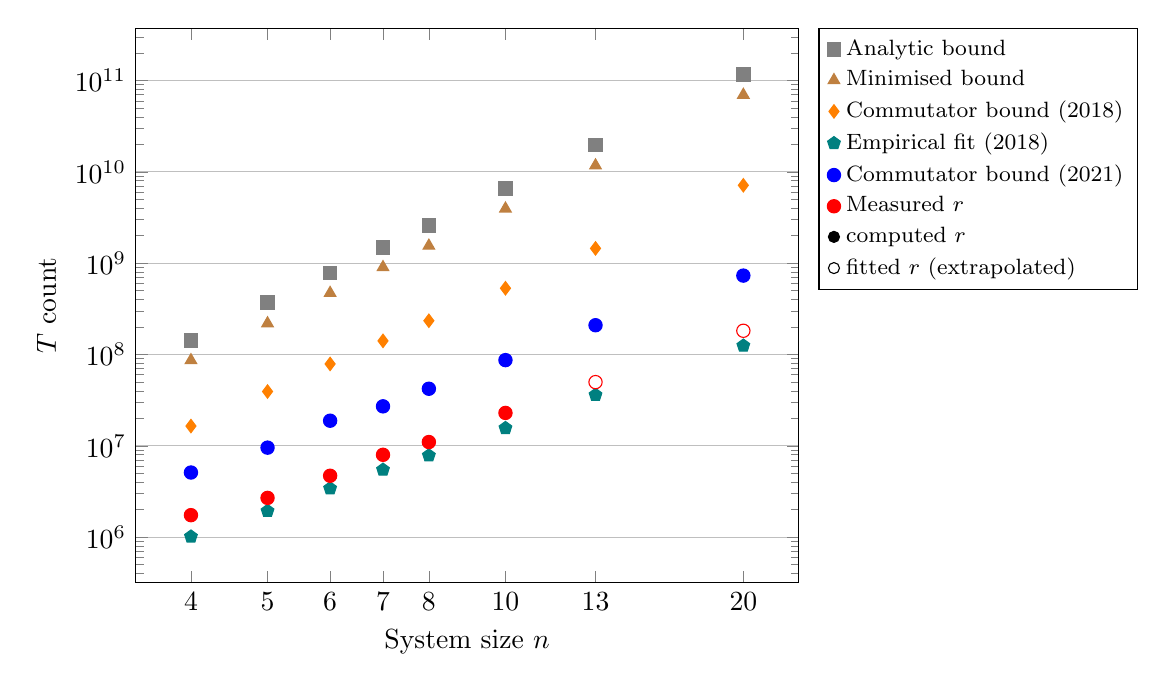
\begin{tikzpicture}
  \begin{loglogaxis}[
    width=10cm,
    xlabel={System size $n$},
    ylabel={$T$ count},
    xtick={4,5,6,7,8,10,13,20},
    xticklabels={4,5,6,7,8,10,13,20},
    ymajorgrids=true,
    legend pos=outer north east,
    legend cell align=left,
    legend style={font=\footnotesize},
  ]
    \addplot[only marks, gray, mark=square*, mark size=2.4pt, mark options={solid, fill=gray}] coordinates {
      (4,142900064)
      (5,369887232)
      (6,783557726)
      (7,1482803784)
      (8,2587232772)
      (10,6588595800)
      (13,19714975684)
      (20,116606541324)
    };
    \addlegendentry{Analytic bound}
    \addplot[only marks, brown, mark=triangle*, mark size=2.4pt, mark options={solid, fill=brown}] coordinates {
      (4,86298624)
      (5,218804960)
      (6,470742840)
      (7,901050280)
      (8,1549621936)
      (10,3953322156)
      (13,11725165980)
      (20,69608829112)
    };
    \addlegendentry{Minimised bound}
    \addplot[only marks, orange, mark=diamond*, mark size=2.4pt, mark options={solid, fill=orange}] coordinates {
      (4,16448124)
      (5,39306456)
      (6,78821280)
      (7,140949800)
      (8,234043080)
      (10,531045440)
      (13,1451578560)
      (20,7125229868)
    };
    \addlegendentry{Commutator bound (2018)}
    \addplot[only marks, teal, mark=pentagon*, mark size=2.4pt, mark options={solid, fill=teal}] coordinates {
      (4,1012782)
      (5,1929754)
      (6,3409920)
      (7,5463920)
      (8,7821000)
      (10,15625418)
      (13,35990730)
      (20,124776288)
    };
    \addlegendentry{Empirical fit (2018)}
    \addplot[only marks, blue, mark=oplus*, mark size=2.4pt, mark options={solid, fill=blue}] coordinates {
      (4,5096824)
      (5,9543744)
      (6,18827328)
      (7,27039896)
      (8,42148120)
      (10,86752020)
      (13,209010544)
      (20,731040960)
    };
    \addlegendentry{Commutator bound (2021)}
    \addplot[only marks, red, mark=*, mark size=2.4pt, mark options={solid, fill=red}] coordinates {
      (4,1739724)
      (5,2687776)
      (6,4698130)
      (7,7969260)
      (8,10989048)
      (10,22900530)
    };
    \addlegendentry{Measured $r$}
    % r from power-law fit (extrapolation); one legend entry per series
    \addplot[only marks, red, mark=*, mark size=2.4pt, mark options={solid, fill=white}, forget plot] coordinates {
      (13,49822284)
      (20,181860528)
    };
    \addlegendimage{only marks, black, mark=*, mark options={fill=black}}
    \addlegendentry{computed $r$}
    \addlegendimage{only marks, black, mark=*, mark options={fill=white}}
    \addlegendentry{fitted $r$ (extrapolated)}
  \end{loglogaxis}
\end{tikzpicture}

\clearpage

\section*{\texttt{t/C-suzuki4-by-bound.tex}}
Suzuki S4: r from each bound and measured\par\medskip
% Generated by pysimcount.pffigure -- do not edit; regenerate instead.
% figure: C-suzuki4-by-bound -- Suzuki S4: r from each bound and measured
% source: results/np-main/seed1/results.json
% metric=t gatebase=ct merged
% seed=1 t=n template=simcount synth=pygridsynth
% git_commit=01d3c275ceae2840002bd1aaea68f59b987c4975 git_dirty=False
% source_sha256=0dd1c9775f148df550d3d3f68cfeee1d2d060b7913324535bbf1533b52b4d2c2
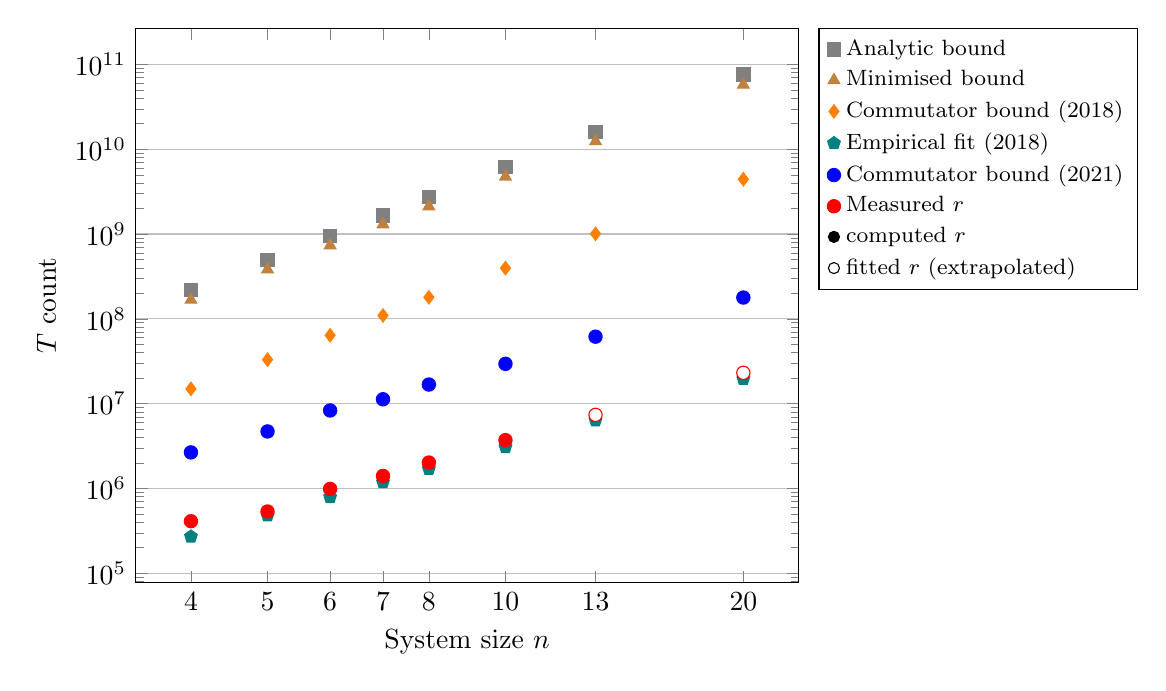
\begin{tikzpicture}
  \begin{loglogaxis}[
    width=10cm,
    xlabel={System size $n$},
    ylabel={$T$ count},
    xtick={4,5,6,7,8,10,13,20},
    xticklabels={4,5,6,7,8,10,13,20},
    ymajorgrids=true,
    legend pos=outer north east,
    legend cell align=left,
    legend style={font=\footnotesize},
  ]
    \addplot[only marks, gray, mark=square*, mark size=2.4pt, mark options={solid, fill=gray}] coordinates {
      (4,217129014)
      (5,490265142)
      (6,947562244)
      (7,1660256568)
      (8,2726214260)
      (10,6171351168)
      (13,15873261390)
      (20,76280562330)
    };
    \addlegendentry{Analytic bound}
    \addplot[only marks, brown, mark=triangle*, mark size=2.4pt, mark options={solid, fill=brown}] coordinates {
      (4,167581482)
      (5,382321536)
      (6,735212988)
      (7,1299472296)
      (8,2117499576)
      (10,4749058800)
      (13,12395182464)
      (20,57627905750)
    };
    \addlegendentry{Minimised bound}
    \addplot[only marks, orange, mark=diamond*, mark size=2.4pt, mark options={solid, fill=orange}] coordinates {
      (4,14953600)
      (5,33012860)
      (6,64032276)
      (7,109665556)
      (8,179648608)
      (10,396099620)
      (13,1006846032)
      (20,4428589536)
    };
    \addlegendentry{Commutator bound (2018)}
    \addplot[only marks, teal, mark=pentagon*, mark size=2.4pt, mark options={solid, fill=teal}] coordinates {
      (4,270410)
      (5,480600)
      (6,790152)
      (7,1183728)
      (8,1698264)
      (10,3073420)
      (13,6353392)
      (20,19508350)
    };
    \addlegendentry{Empirical fit (2018)}
    \addplot[only marks, blue, mark=oplus*, mark size=2.4pt, mark options={solid, fill=blue}] coordinates {
      (4,2661098)
      (5,4701024)
      (6,8314572)
      (7,11267100)
      (8,16796502)
      (10,29484208)
      (13,61637022)
      (20,178374976)
    };
    \addlegendentry{Commutator bound (2021)}
    \addplot[only marks, red, mark=*, mark size=2.4pt, mark options={solid, fill=red}] coordinates {
      (4,410856)
      (5,534710)
      (6,987026)
      (7,1404340)
      (8,2020560)
      (10,3710728)
    };
    \addlegendentry{Measured $r$}
    % r from power-law fit (extrapolation); one legend entry per series
    \addplot[only marks, red, mark=*, mark size=2.4pt, mark options={solid, fill=white}, forget plot] coordinates {
      (13,7377150)
      (20,23100384)
    };
    \addlegendimage{only marks, black, mark=*, mark options={fill=black}}
    \addlegendentry{computed $r$}
    \addlegendimage{only marks, black, mark=*, mark options={fill=white}}
    \addlegendentry{fitted $r$ (extrapolated)}
  \end{loglogaxis}
\end{tikzpicture}

\clearpage

\section*{\texttt{t/C-suzuki6-by-bound.tex}}
Suzuki S6: r from each bound and measured\par\medskip
% Generated by plsimcount.pffigure -- do not edit; regenerate instead.
% figure: C-suzuki6-by-bound -- Suzuki S6: r from each bound and measured
% source: results/np-main/seed1/results.json
% metric=t gatebase=ct merged
% seed=1 t=n template=simcount synth=pygridsynth
% git_commit=01d3c275ceae2840002bd1aaea68f59b987c4975 git_dirty=False
% source_sha256=0dd1c9775f148df550d3d3f68cfeee1d2d060b7913324535bbf1533b52b4d2c2
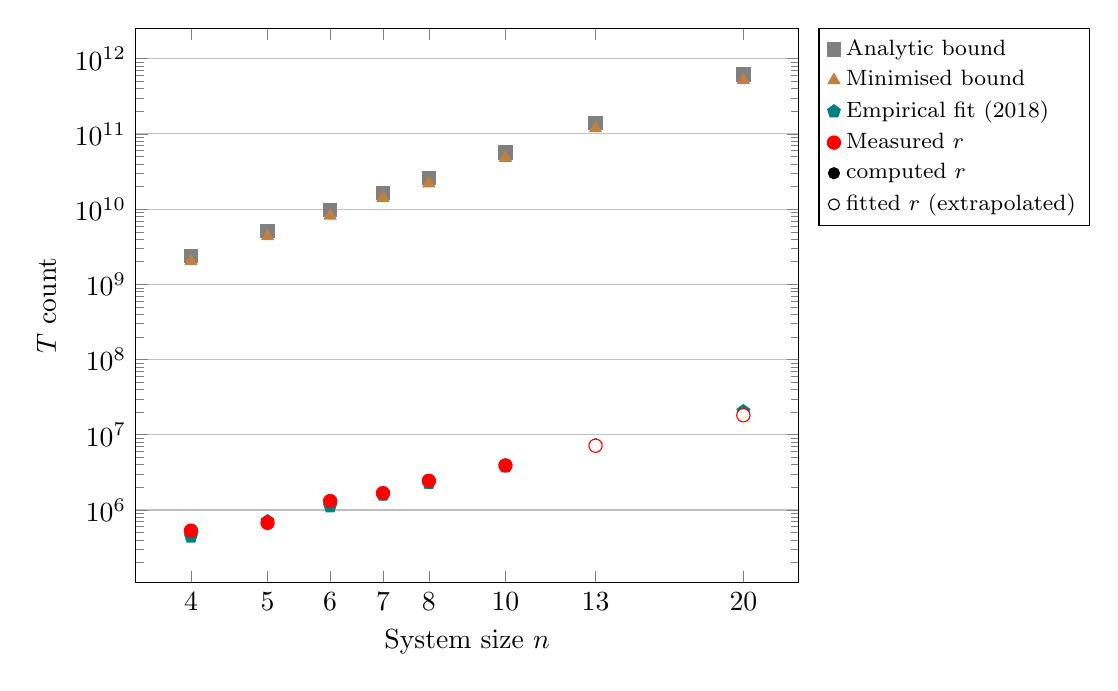
\begin{tikzpicture}
  \begin{loglogaxis}[
    width=10cm,
    xlabel={System size $n$},
    ylabel={$T$ count},
    xtick={4,5,6,7,8,10,13,20},
    xticklabels={4,5,6,7,8,10,13,20},
    ymajorgrids=true,
    legend pos=outer north east,
    legend cell align=left,
    legend style={font=\footnotesize},
  ]
    \addplot[only marks, gray, mark=square*, mark size=2.4pt, mark options={solid, fill=gray}] coordinates {
      (4,2367809968)
      (5,5097618340)
      (6,9714995620)
      (7,16373298184)
      (8,26078648328)
      (10,56517973560)
      (13,139918929000)
      (20,618368280168)
    };
    \addlegendentry{Analytic bound}
    \addplot[only marks, brown, mark=triangle*, mark size=2.4pt, mark options={solid, fill=brown}] coordinates {
      (4,2024782542)
      (5,4360753356)
      (6,8172748976)
      (7,14055074646)
      (8,22006049912)
      (10,48017099500)
      (13,118696724096)
      (20,521672145806)
    };
    \addlegendentry{Minimised bound}
    \addplot[only marks, teal, mark=pentagon*, mark size=2.4pt, mark options={solid, fill=teal}] coordinates {
      (4,442560)
      (5,709620)
      (6,1118188)
      (7,1599282)
      (8,2296392)
      (10,3800566)
      (13,7287904)
      (20,20534332)
    };
    \addlegendentry{Empirical fit (2018)}
    \addplot[only marks, red, mark=*, mark size=2.4pt, mark options={solid, fill=red}] coordinates {
      (4,530964)
      (5,673708)
      (6,1314412)
      (7,1673760)
      (8,2443080)
      (10,3919244)
    };
    \addlegendentry{Measured $r$}
    % r from power-law fit (extrapolation); one legend entry per series
    \addplot[only marks, red, mark=*, mark size=2.4pt, mark options={solid, fill=white}, forget plot] coordinates {
      (13,7156932)
      (20,18178252)
    };
    \addlegendimage{only marks, black, mark=*, mark options={fill=black}}
    \addlegendentry{computed $r$}
    \addlegendimage{only marks, black, mark=*, mark options={fill=white}}
    \addlegendentry{fitted $r$ (extrapolated)}
  \end{loglogaxis}
\end{tikzpicture}

\clearpage

\section*{\texttt{t/C-suzuki8-by-bound.tex}}
Suzuki S8: r from each bound and measured\par\medskip
% Generated by pysimcount.pffigure -- do not edit; regenerate instead.
% figure: C-suzuki8-by-bound -- Suzuki S8: r from each bound and measured
% source: results/np-main/seed1/results.json
% metric=t gatebase=ct merged
% seed=1 t=n template=simcount synth=pygridsynth
% git_commit=01d3c275ceae2840002bd1aaea68f59b987c4975 git_dirty=False
% source_sha256=0dd1c9775f148df550d3d3f68cfeee1d2d060b7913324535bbf1533b52b4d2c2
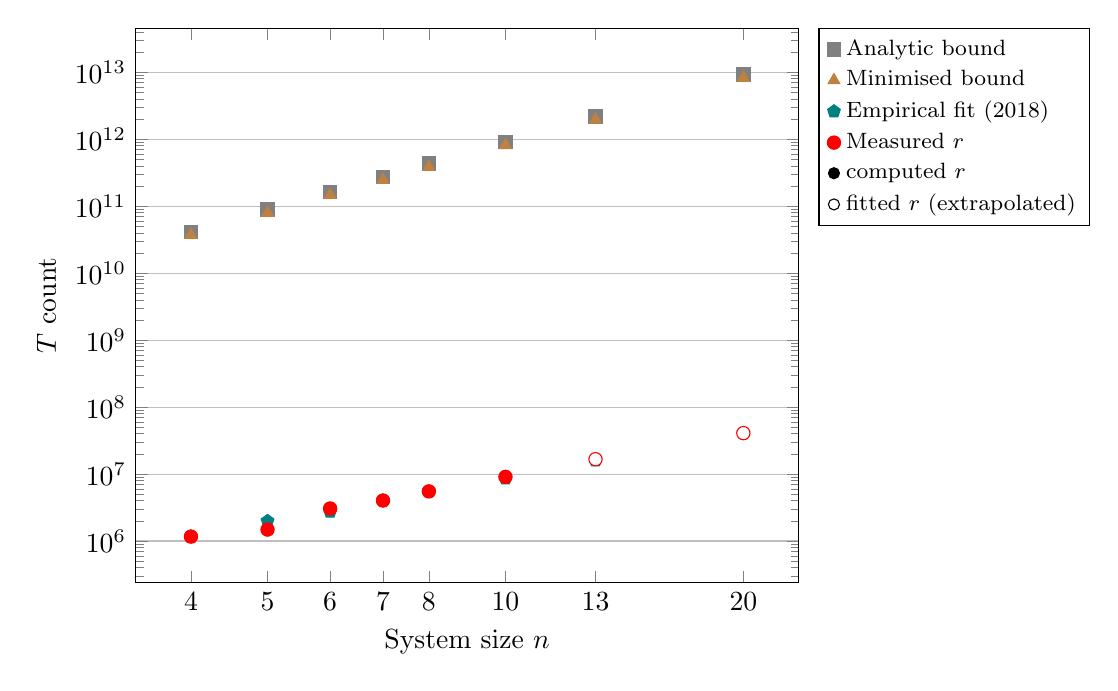
\begin{tikzpicture}
  \begin{loglogaxis}[
    width=10cm,
    xlabel={System size $n$},
    ylabel={$T$ count},
    xtick={4,5,6,7,8,10,13,20},
    xticklabels={4,5,6,7,8,10,13,20},
    ymajorgrids=true,
    legend pos=outer north east,
    legend cell align=left,
    legend style={font=\footnotesize},
  ]
    \addplot[only marks, gray, mark=square*, mark size=2.4pt, mark options={solid, fill=gray}] coordinates {
      (4,41351550240)
      (5,89126606142)
      (6,162780181776)
      (7,274661490840)
      (8,431167981430)
      (10,904986121032)
      (13,2187588939552)
      (20,9258138748774)
    };
    \addlegendentry{Analytic bound}
    \addplot[only marks, brown, mark=triangle*, mark size=2.4pt, mark options={solid, fill=brown}] coordinates {
      (4,37023325728)
      (5,79151533952)
      (6,146176022952)
      (7,245258541836)
      (8,382948701696)
      (10,811163790000)
      (13,1950511504920)
      (20,8207330049928)
    };
    \addlegendentry{Minimised bound}
    \addplot[only marks, teal, mark=pentagon*, mark size=2.4pt, mark options={solid, fill=teal}] coordinates {
      (4,1164552)
      (5,1986752)
      (6,2741688)
      (7,4023074)
      (8,5513378)
      (10,8632000)
      (13,15967908)
      (20,40825400)
    };
    \addlegendentry{Empirical fit (2018)}
    \addplot[only marks, red, mark=*, mark size=2.4pt, mark options={solid, fill=red}] coordinates {
      (4,1164552)
      (5,1483068)
      (6,3062680)
      (7,4023074)
      (8,5513378)
      (10,9073036)
    };
    \addlegendentry{Measured $r$}
    % r from power-law fit (extrapolation); one legend entry per series
    \addplot[only marks, red, mark=*, mark size=2.4pt, mark options={solid, fill=white}, forget plot] coordinates {
      (13,16651540)
      (20,40825400)
    };
    \addlegendimage{only marks, black, mark=*, mark options={fill=black}}
    \addlegendentry{computed $r$}
    \addlegendimage{only marks, black, mark=*, mark options={fill=white}}
    \addlegendentry{fitted $r$ (extrapolated)}
  \end{loglogaxis}
\end{tikzpicture}

\clearpage

\section*{\texttt{total/A-ana-by-order.tex}}
Suzuki formulas of each order, r from: Analytic bound\par\medskip
% Generated by pysimcount.pffigure -- do not edit; regenerate instead.
% figure: A-ana-by-order -- Suzuki formulas of each order, r from: Analytic bound
% source: results/np-main/seed1/results.json
% metric=total gatebase=cz merged
% seed=1 t=n template=simcount synth=pygridsynth
% git_commit=01d3c275ceae2840002bd1aaea68f59b987c4975 git_dirty=False
% source_sha256=0dd1c9775f148df550d3d3f68cfeee1d2d060b7913324535bbf1533b52b4d2c2
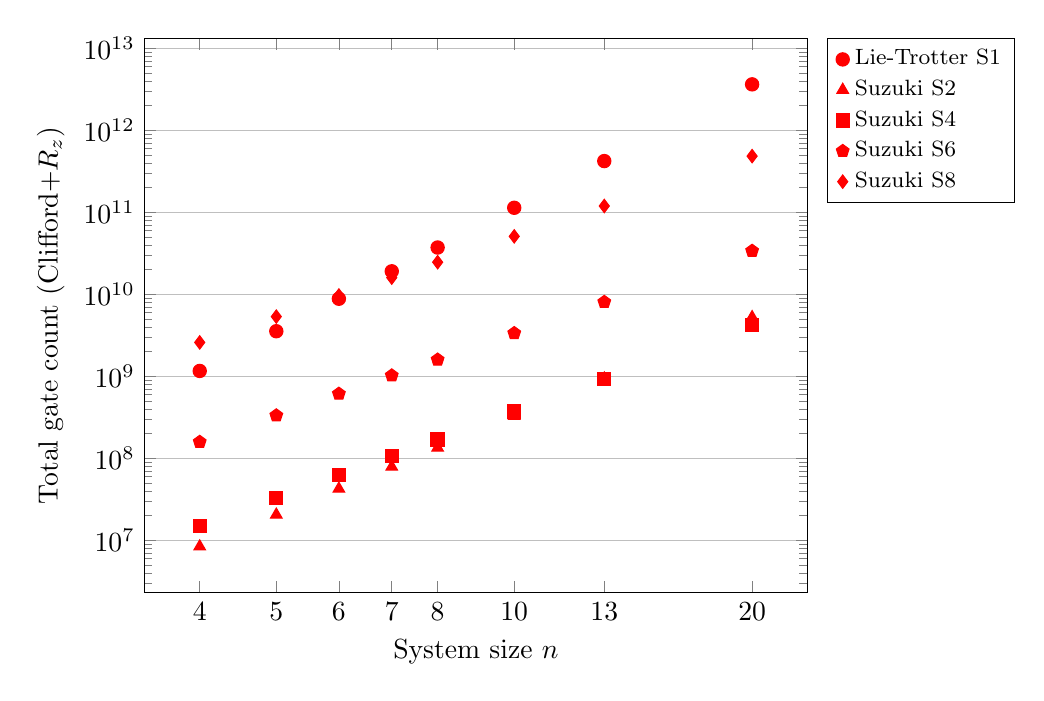
\begin{tikzpicture}
  \begin{loglogaxis}[
    width=10cm,
    xlabel={System size $n$},
    ylabel={Total gate count (Clifford+$R_z$)},
    xtick={4,5,6,7,8,10,13,20},
    xticklabels={4,5,6,7,8,10,13,20},
    ymajorgrids=true,
    legend pos=outer north east,
    legend cell align=left,
    legend style={font=\footnotesize},
  ]
    \addplot[only marks, red, mark=*, mark size=2.4pt, mark options={solid, fill=red}] coordinates {
      (4,1157944632)
      (5,3533766470)
      (6,8793141552)
      (7,19005443730)
      (8,37054226144)
      (10,113080524180)
      (13,419860070266)
      (20,3618576770120)
    };
    \addlegendentry{Lie-Trotter S1}
    \addplot[only marks, red, mark=triangle*, mark size=2.4pt, mark options={solid, fill=red}] coordinates {
      (4,8369664)
      (5,20433600)
      (6,42371136)
      (7,78497664)
      (8,133913088)
      (10,326936160)
      (13,933762336)
      (20,5230977600)
    };
    \addlegendentry{Suzuki S2}
    \addplot[only marks, red, mark=square*, mark size=2.4pt, mark options={solid, fill=red}] coordinates {
      (4,14977376)
      (5,32704180)
      (6,61906968)
      (7,106181684)
      (8,169442272)
      (10,370003600)
      (13,926842800)
      (20,4186096880)
    };
    \addlegendentry{Suzuki S4}
    \addplot[only marks, red, mark=pentagon*, mark size=2.4pt, mark options={solid, fill=red}] coordinates {
      (4,157743264)
      (5,331880880)
      (6,609422832)
      (7,1018757376)
      (8,1589932224)
      (10,3345114480)
      (13,8020876344)
      (20,33716595840)
    };
    \addlegendentry{Suzuki S6}
    \addplot[only marks, red, mark=diamond*, mark size=2.4pt, mark options={solid, fill=red}] coordinates {
      (4,2580061680)
      (5,5328273340)
      (6,9636633528)
      (7,15903842192)
      (8,24545740160)
      (10,50691330000)
      (13,118918467928)
      (20,482259582560)
    };
    \addlegendentry{Suzuki S8}
  \end{loglogaxis}
\end{tikzpicture}

\clearpage

\section*{\texttt{total/A-min-by-order.tex}}
Suzuki formulas of each order, r from: Minimised bound\par\medskip
% Generated by plsimcount.pffigure -- do not edit; regenerate instead.
% figure: A-min-by-order -- Suzuki formulas of each order, r from: Minimised bound
% source: results/np-main/seed1/results.json
% metric=total gatebase=cz merged
% seed=1 t=n template=simcount synth=pygridsynth
% git_commit=01d3c275ceae2840002bd1aaea68f59b987c4975 git_dirty=False
% source_sha256=0dd1c9775f148df550d3d3f68cfeee1d2d060b7913324535bbf1533b52b4d2c2
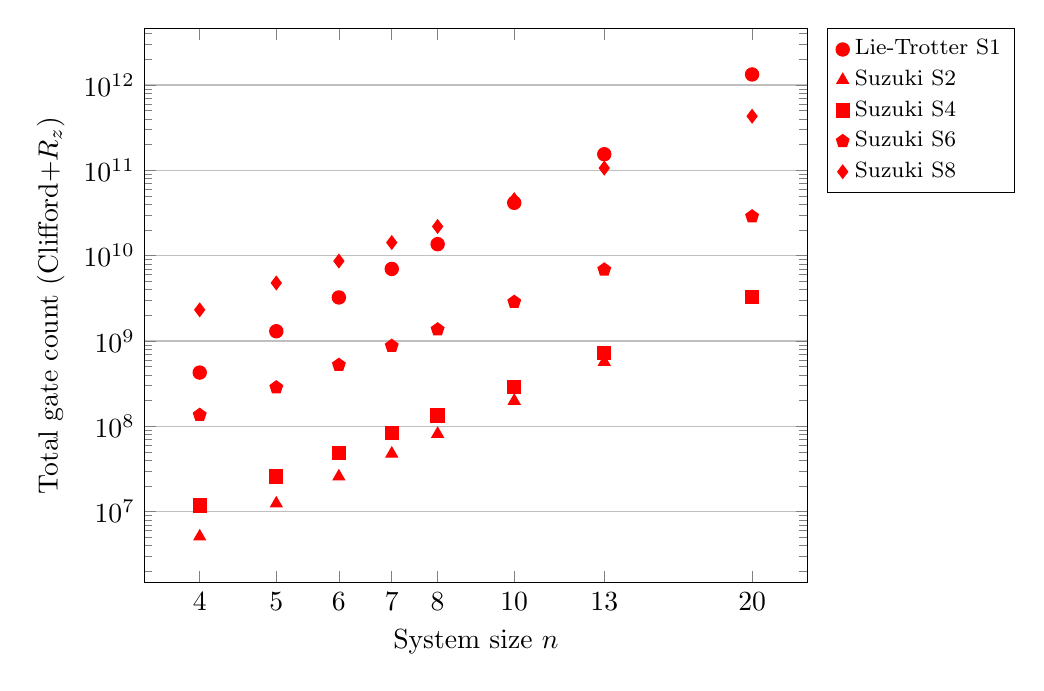
\begin{tikzpicture}
  \begin{loglogaxis}[
    width=10cm,
    xlabel={System size $n$},
    ylabel={Total gate count (Clifford+$R_z$)},
    xtick={4,5,6,7,8,10,13,20},
    xticklabels={4,5,6,7,8,10,13,20},
    ymajorgrids=true,
    legend pos=outer north east,
    legend cell align=left,
    legend style={font=\footnotesize},
  ]
    \addplot[only marks, red, mark=*, mark size=2.4pt, mark options={solid, fill=red}] coordinates {
      (4,425990656)
      (5,1300013000)
      (6,3234838464)
      (7,6991747672)
      (8,13631541248)
      (10,41600104000)
      (13,154458116488)
      (20,1331200832000)
    };
    \addlegendentry{Lie-Trotter S1}
    \addplot[only marks, red, mark=triangle*, mark size=2.4pt, mark options={solid, fill=red}] coordinates {
      (4,5088768)
      (5,12417600)
      (6,25740864)
      (7,47677056)
      (8,81320832)
      (10,198489120)
      (13,566777328)
      (20,3174284160)
    };
    \addlegendentry{Suzuki S2}
    \addplot[only marks, red, mark=square*, mark size=2.4pt, mark options={solid, fill=red}] coordinates {
      (4,11799072)
      (5,25733620)
      (6,48669264)
      (7,83418608)
      (8,133042720)
      (10,290270400)
      (13,726470576)
      (20,3277053600)
    };
    \addlegendentry{Suzuki S4}
    \addplot[only marks, red, mark=pentagon*, mark size=2.4pt, mark options={solid, fill=red}] coordinates {
      (4,135712128)
      (5,285198360)
      (6,523242576)
      (7,874082328)
      (8,1363346304)
      (10,2865771120)
      (13,6864685464)
      (20,28814368800)
    };
    \addlegendentry{Suzuki S6}
    \addplot[only marks, red, mark=diamond*, mark size=2.4pt, mark options={solid, fill=red}] coordinates {
      (4,2317590672)
      (5,4781715340)
      (6,8641774800)
      (7,14253457708)
      (8,21987540800)
      (10,45371909360)
      (13,106345237284)
      (20,430694067680)
    };
    \addlegendentry{Suzuki S8}
  \end{loglogaxis}
\end{tikzpicture}

\clearpage

\section*{\texttt{total/A-com-by-order.tex}}
Suzuki formulas of each order, r from: Commutator bound (2018)\par\medskip
% Generated by pysimcount.pffigure -- do not edit; regenerate instead.
% figure: A-com-by-order -- Suzuki formulas of each order, r from: Commutator bound (2018)
% source: results/np-main/seed1/results.json
% metric=total gatebase=cz merged
% seed=1 t=n template=simcount synth=pygridsynth
% git_commit=01d3c275ceae2840002bd1aaea68f59b987c4975 git_dirty=False
% source_sha256=0dd1c9775f148df550d3d3f68cfeee1d2d060b7913324535bbf1533b52b4d2c2
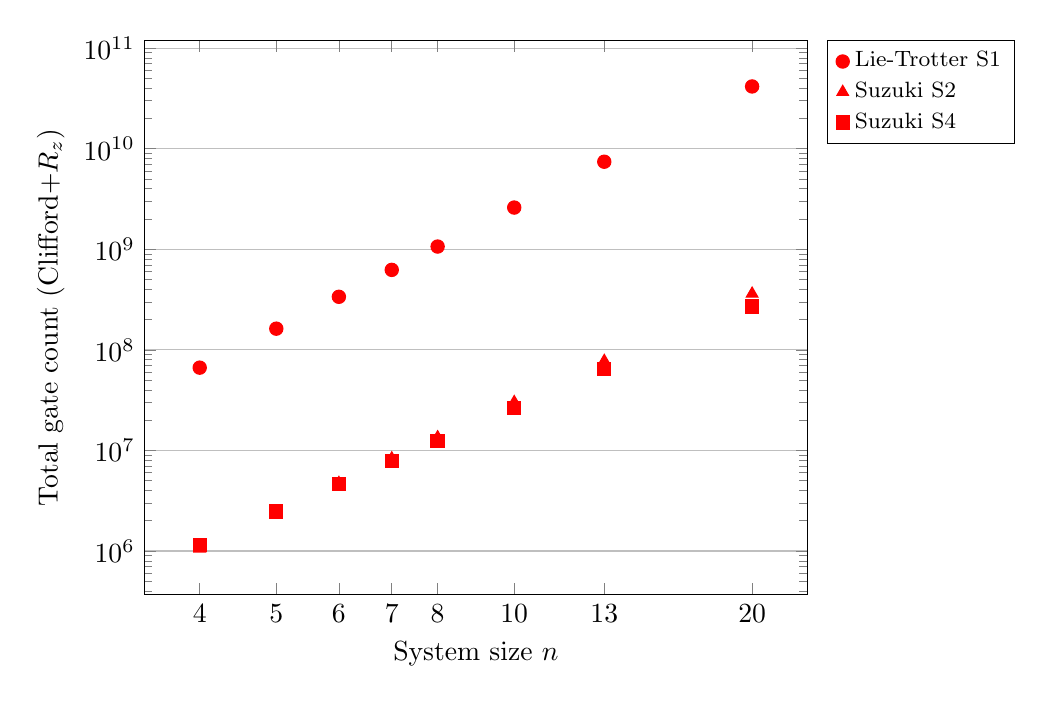
\begin{tikzpicture}
  \begin{loglogaxis}[
    width=10cm,
    xlabel={System size $n$},
    ylabel={Total gate count (Clifford+$R_z$)},
    xtick={4,5,6,7,8,10,13,20},
    xticklabels={4,5,6,7,8,10,13,20},
    ymajorgrids=true,
    legend pos=outer north east,
    legend cell align=left,
    legend style={font=\footnotesize},
  ]
    \addplot[only marks, red, mark=*, mark size=2.4pt, mark options={solid, fill=red}] coordinates {
      (4,66574248)
      (5,162534710)
      (6,337031916)
      (7,624393224)
      (8,1065187344)
      (10,2600554580)
      (13,7427444206)
      (20,41608873280)
    };
    \addlegendentry{Lie-Trotter S1}
    \addplot[only marks, red, mark=triangle*, mark size=2.4pt, mark options={solid, fill=red}] coordinates {
      (4,1056576)
      (5,2426400)
      (6,4743648)
      (7,8324064)
      (8,13512960)
      (10,30239040)
      (13,77585040)
      (20,361881600)
    };
    \addlegendentry{Suzuki S2}
    \addplot[only marks, red, mark=square*, mark size=2.4pt, mark options={solid, fill=red}] coordinates {
      (4,1143952)
      (5,2475100)
      (6,4635168)
      (7,7862232)
      (8,12404544)
      (10,26468200)
      (13,64126608)
      (20,270766400)
    };
    \addlegendentry{Suzuki S4}
  \end{loglogaxis}
\end{tikzpicture}

\clearpage

\section*{\texttt{total/A-emp-by-order.tex}}
Suzuki formulas of each order, r from: Empirical fit (2018)\par\medskip
% Generated by plsimcount.pffigure -- do not edit; regenerate instead.
% figure: A-emp-by-order -- Suzuki formulas of each order, r from: Empirical fit (2018)
% source: results/np-main/seed1/results.json
% metric=total gatebase=cz merged
% seed=1 t=n template=simcount synth=pygridsynth
% git_commit=01d3c275ceae2840002bd1aaea68f59b987c4975 git_dirty=False
% source_sha256=0dd1c9775f148df550d3d3f68cfeee1d2d060b7913324535bbf1533b52b4d2c2
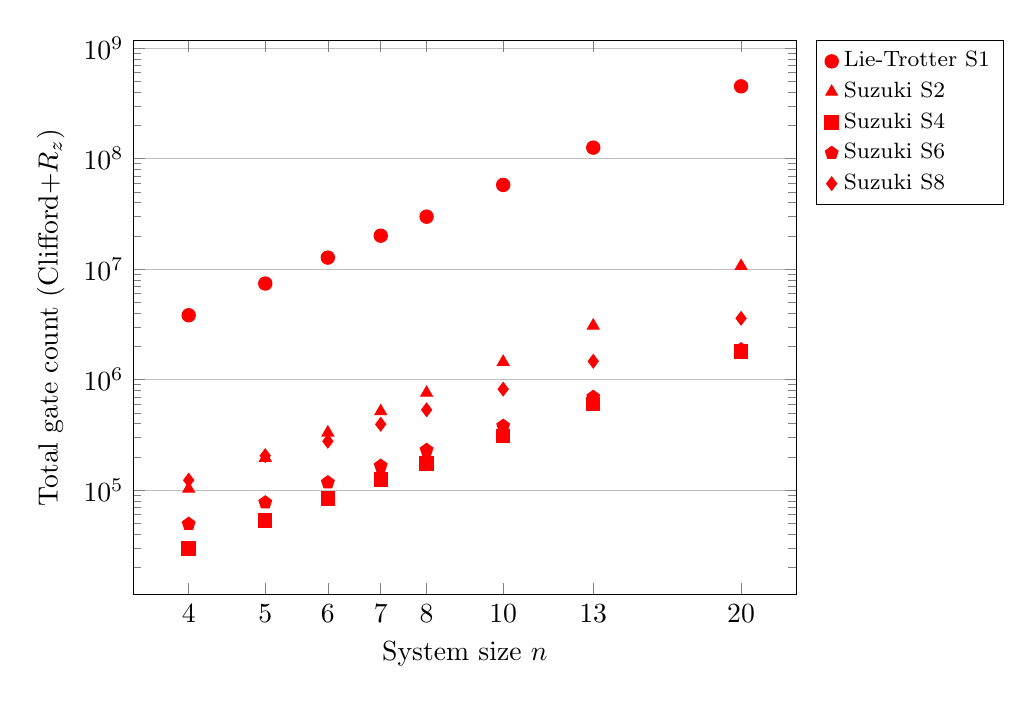
\begin{tikzpicture}
  \begin{loglogaxis}[
    width=10cm,
    xlabel={System size $n$},
    ylabel={Total gate count (Clifford+$R_z$)},
    xtick={4,5,6,7,8,10,13,20},
    xticklabels={4,5,6,7,8,10,13,20},
    ymajorgrids=true,
    legend pos=outer north east,
    legend cell align=left,
    legend style={font=\footnotesize},
  ]
    \addplot[only marks, red, mark=*, mark size=2.4pt, mark options={solid, fill=red}] coordinates {
      (4,3826576)
      (5,7413900)
      (6,12727572)
      (7,20098988)
      (8,29857984)
      (10,57850000)
      (13,125901958)
      (20,451398480)
    };
    \addlegendentry{Lie-Trotter S1}
    \addplot[only marks, red, mark=triangle*, mark size=2.4pt, mark options={solid, fill=red}] coordinates {
      (4,103104)
      (5,196080)
      (6,331776)
      (7,517440)
      (8,760320)
      (10,1446240)
      (13,3080688)
      (20,10664640)
    };
    \addlegendentry{Suzuki S2}
    \addplot[only marks, red, mark=square*, mark size=2.4pt, mark options={solid, fill=red}] coordinates {
      (4,29680)
      (5,53000)
      (6,83952)
      (7,124656)
      (8,174688)
      (10,307400)
      (13,600808)
      (20,1802000)
    };
    \addlegendentry{Suzuki S4}
    \addplot[only marks, red, mark=pentagon*, mark size=2.4pt, mark options={solid, fill=red}] coordinates {
      (4,49536)
      (5,77400)
      (6,117648)
      (7,166152)
      (8,231168)
      (10,381840)
      (13,697632)
      (20,1878240)
    };
    \addlegendentry{Suzuki S6}
    \addplot[only marks, red, mark=diamond*, mark size=2.4pt, mark options={solid, fill=red}] coordinates {
      (4,123168)
      (5,205280)
      (6,277128)
      (7,395164)
      (8,533728)
      (10,821120)
      (13,1467752)
      (20,3592400)
    };
    \addlegendentry{Suzuki S8}
  \end{loglogaxis}
\end{tikzpicture}

\clearpage

\section*{\texttt{total/A-tte-by-order.tex}}
Suzuki formulas of each order, r from: Commutator bound (2021)\par\medskip
% Generated by plsimcount.pffigure -- do not edit; regenerate instead.
% figure: A-tte-by-order -- Suzuki formulas of each order, r from: Commutator bound (2021)
% source: results/np-main/seed1/results.json
% metric=total gatebase=cz merged
% seed=1 t=n template=simcount synth=pygridsynth
% git_commit=01d3c275ceae2840002bd1aaea68f59b987c4975 git_dirty=False
% source_sha256=0dd1c9775f148df550d3d3f68cfeee1d2d060b7913324535bbf1533b52b4d2c2
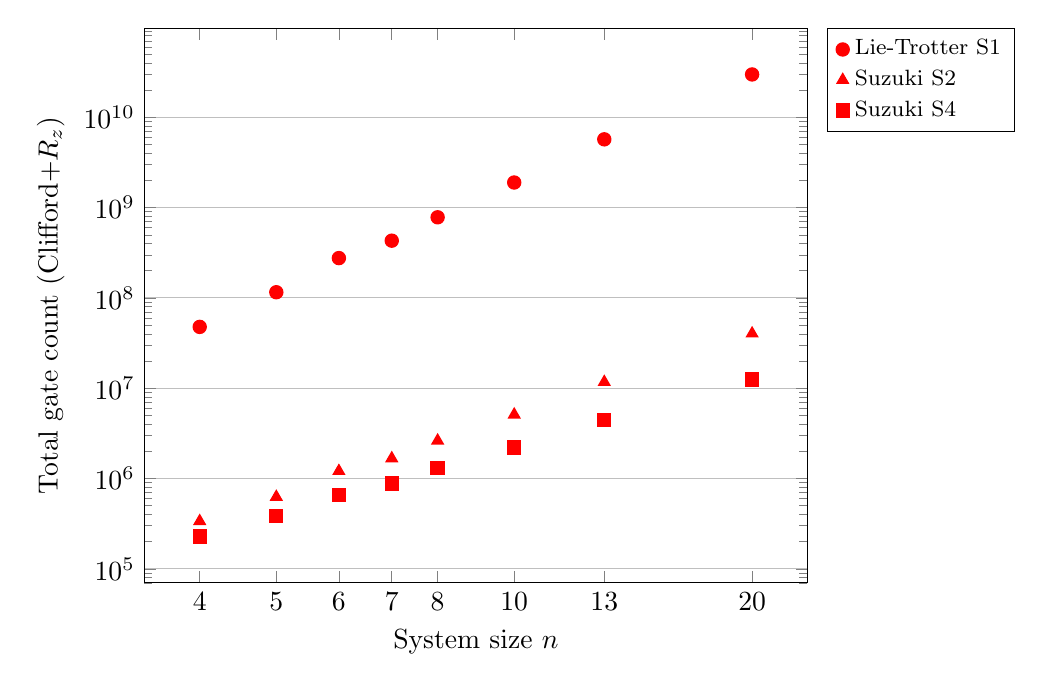
\begin{tikzpicture}
  \begin{loglogaxis}[
    width=10cm,
    xlabel={System size $n$},
    ylabel={Total gate count (Clifford+$R_z$)},
    xtick={4,5,6,7,8,10,13,20},
    xticklabels={4,5,6,7,8,10,13,20},
    ymajorgrids=true,
    legend pos=outer north east,
    legend cell align=left,
    legend style={font=\footnotesize},
  ]
    \addplot[only marks, red, mark=*, mark size=2.4pt, mark options={solid, fill=red}] coordinates {
      (4,47754616)
      (5,115578970)
      (6,276106740)
      (7,430452022)
      (8,781371760)
      (10,1897292540)
      (13,5702423688)
      (20,29845046920)
    };
    \addlegendentry{Lie-Trotter S1}
    \addplot[only marks, red, mark=triangle*, mark size=2.4pt, mark options={solid, fill=red}] coordinates {
      (4,336576)
      (5,624960)
      (6,1207296)
      (7,1669584)
      (8,2625024)
      (10,5094240)
      (13,11694384)
      (20,40241280)
    };
    \addlegendentry{Suzuki S2}
    \addplot[only marks, red, mark=square*, mark size=2.4pt, mark options={solid, fill=red}] coordinates {
      (4,227264)
      (5,384780)
      (6,661440)
      (7,877044)
      (8,1297440)
      (10,2206920)
      (13,4464720)
      (20,12465600)
    };
    \addlegendentry{Suzuki S4}
  \end{loglogaxis}
\end{tikzpicture}

\clearpage

\section*{\texttt{total/A-measured-by-order.tex}}
Suzuki formulas of each order, r from: Measured $r$\par\medskip
% Generated by pysimcount.pffigure -- do not edit; regenerate instead.
% figure: A-measured-by-order -- Suzuki formulas of each order, r from: Measured $r$
% source: results/np-main/seed1/results.json
% metric=total gatebase=cz merged
% seed=1 t=n template=simcount synth=pygridsynth
% git_commit=01d3c275ceae2840002bd1aaea68f59b987c4975 git_dirty=False
% source_sha256=0dd1c9775f148df550d3d3f68cfeee1d2d060b7913324535bbf1533b52b4d2c2
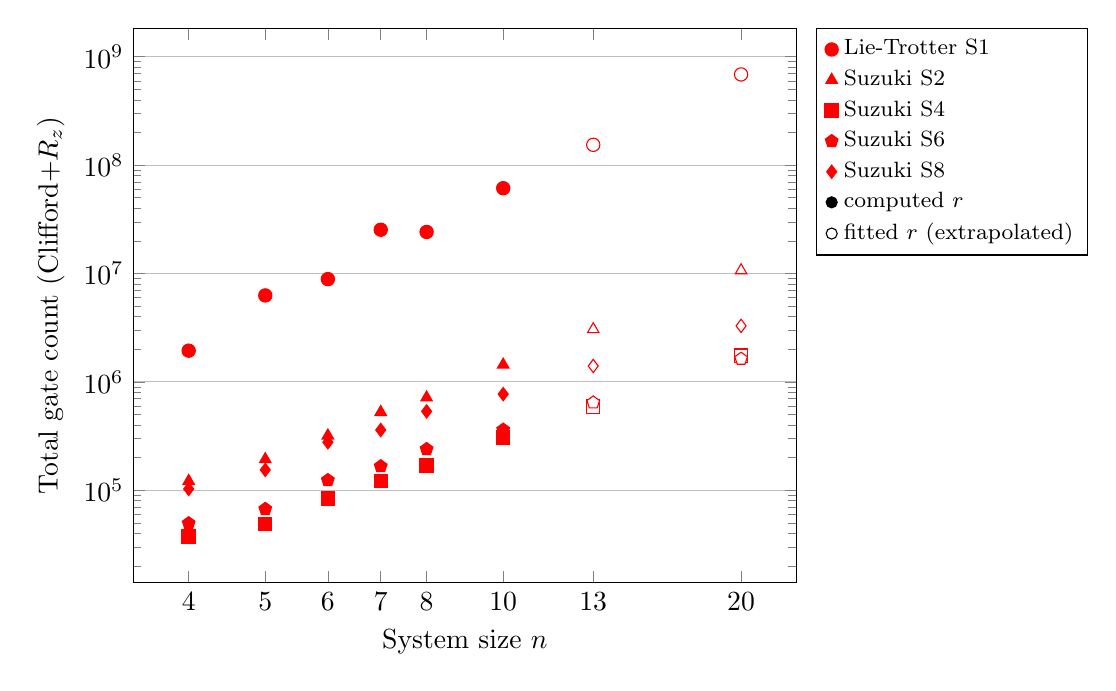
\begin{tikzpicture}
  \begin{loglogaxis}[
    width=10cm,
    xlabel={System size $n$},
    ylabel={Total gate count (Clifford+$R_z$)},
    xtick={4,5,6,7,8,10,13,20},
    xticklabels={4,5,6,7,8,10,13,20},
    ymajorgrids=true,
    legend pos=outer north east,
    legend cell align=left,
    legend style={font=\footnotesize},
  ]
    \addplot[only marks, red, mark=*, mark size=2.4pt, mark options={solid, fill=red}] coordinates {
      (4,1939704)
      (5,6273410)
      (6,8873592)
      (7,25339496)
      (8,24174384)
      (10,61219080)
    };
    \addlegendentry{Lie-Trotter S1}
    % r from power-law fit (extrapolation); one legend entry per series
    \addplot[only marks, red, mark=*, mark size=2.4pt, mark options={solid, fill=white}, forget plot] coordinates {
      (13,153917426)
      (20,686838880)
    };
    \addplot[only marks, red, mark=triangle*, mark size=2.4pt, mark options={solid, fill=red}] coordinates {
      (4,121344)
      (5,192720)
      (6,318816)
      (7,525168)
      (8,715392)
      (10,1437120)
    };
    \addlegendentry{Suzuki S2}
    % r from power-law fit (extrapolation); one legend entry per series
    \addplot[only marks, red, mark=triangle*, mark size=2.4pt, mark options={solid, fill=white}, forget plot] coordinates {
      (13,3051360)
      (20,10674240)
    };
    \addplot[only marks, red, mark=square*, mark size=2.4pt, mark options={solid, fill=red}] coordinates {
      (4,37312)
      (5,48760)
      (6,83952)
      (7,121688)
      (8,169600)
      (10,305280)
    };
    \addlegendentry{Suzuki S4}
    % r from power-law fit (extrapolation); one legend entry per series
    \addplot[only marks, red, mark=square*, mark size=2.4pt, mark options={solid, fill=white}, forget plot] coordinates {
      (13,589784)
      (20,1746880)
    };
    \addplot[only marks, red, mark=pentagon*, mark size=2.4pt, mark options={solid, fill=red}] coordinates {
      (4,49536)
      (5,67080)
      (6,123840)
      (7,166152)
      (8,239424)
      (10,361200)
    };
    \addlegendentry{Suzuki S6}
    % r from power-law fit (extrapolation); one legend entry per series
    \addplot[only marks, red, mark=pentagon*, mark size=2.4pt, mark options={solid, fill=white}, forget plot] coordinates {
      (13,643968)
      (20,1630560)
    };
    \addplot[only marks, red, mark=diamond*, mark size=2.4pt, mark options={solid, fill=red}] coordinates {
      (4,102640)
      (5,153960)
      (6,277128)
      (7,359240)
      (8,533728)
      (10,769800)
    };
    \addlegendentry{Suzuki S8}
    % r from power-law fit (extrapolation); one legend entry per series
    \addplot[only marks, red, mark=diamond*, mark size=2.4pt, mark options={solid, fill=white}, forget plot] coordinates {
      (13,1401036)
      (20,3284480)
    };
    \addlegendimage{only marks, black, mark=*, mark options={fill=black}}
    \addlegendentry{computed $r$}
    \addlegendimage{only marks, black, mark=*, mark options={fill=white}}
    \addlegendentry{fitted $r$ (extrapolated)}
  \end{loglogaxis}
\end{tikzpicture}

\clearpage

\section*{\texttt{total/B-order4-by-formula.tex}}
Every order-4 formula at measured r\par\medskip
% Generated by plsimcount.pffigure -- do not edit; regenerate instead.
% figure: B-order4-by-formula -- Every order-4 formula at measured r
% source: results/np-main/seed1/results.json
% metric=total gatebase=cz merged
% seed=1 t=n template=simcount synth=pygridsynth
% git_commit=01d3c275ceae2840002bd1aaea68f59b987c4975 git_dirty=False
% source_sha256=0dd1c9775f148df550d3d3f68cfeee1d2d060b7913324535bbf1533b52b4d2c2
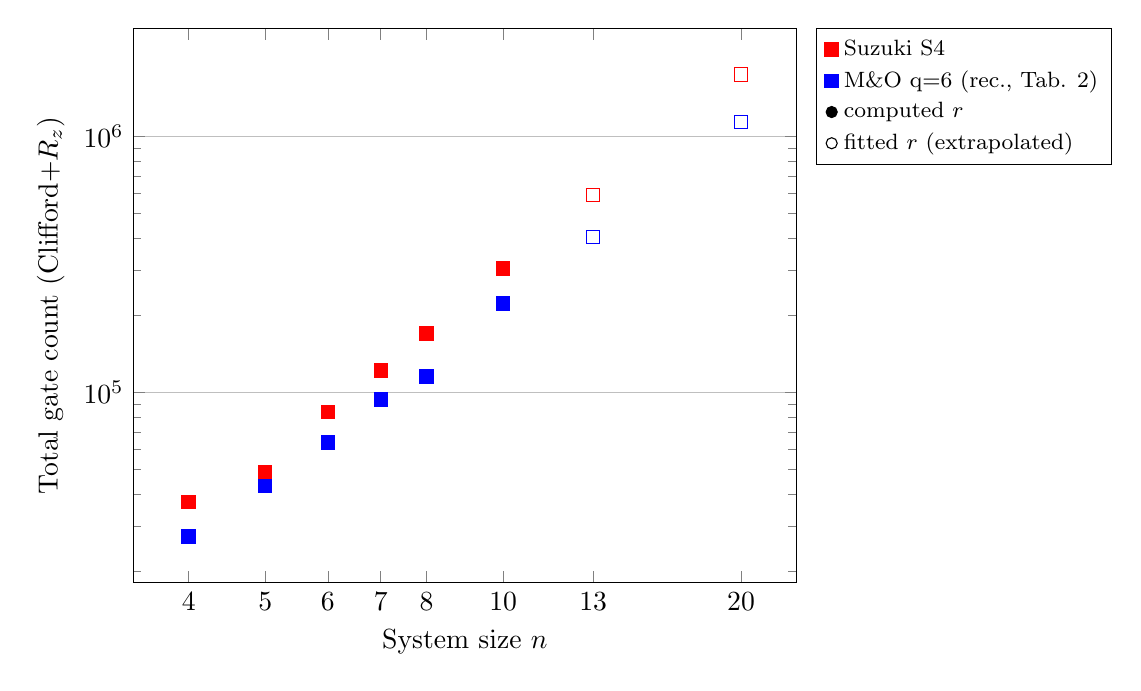
\begin{tikzpicture}
  \begin{loglogaxis}[
    width=10cm,
    xlabel={System size $n$},
    ylabel={Total gate count (Clifford+$R_z$)},
    xtick={4,5,6,7,8,10,13,20},
    xticklabels={4,5,6,7,8,10,13,20},
    ymajorgrids=true,
    legend pos=outer north east,
    legend cell align=left,
    legend style={font=\footnotesize},
  ]
    \addplot[only marks, red, mark=square*, mark size=2.4pt, mark options={solid, fill=red}] coordinates {
      (4,37312)
      (5,48760)
      (6,83952)
      (7,121688)
      (8,169600)
      (10,305280)
    };
    \addlegendentry{Suzuki S4}
    % r from power-law fit (extrapolation); one legend entry per series
    \addplot[only marks, red, mark=square*, mark size=2.4pt, mark options={solid, fill=white}, forget plot] coordinates {
      (13,589784)
      (20,1746880)
    };
    \addplot[only marks, blue, mark=square*, mark size=2.4pt, mark options={solid, fill=blue}] coordinates {
      (4,27324)
      (5,43010)
      (6,63756)
      (7,93863)
      (8,115368)
      (10,222640)
    };
    \addlegendentry{M\&O q=6 (rec., Tab. 2)}
    % r from power-law fit (extrapolation); one legend entry per series
    \addplot[only marks, blue, mark=square*, mark size=2.4pt, mark options={solid, fill=white}, forget plot] coordinates {
      (13,404547)
      (20,1138500)
    };
    \addlegendimage{only marks, black, mark=*, mark options={fill=black}}
    \addlegendentry{computed $r$}
    \addlegendimage{only marks, black, mark=*, mark options={fill=white}}
    \addlegendentry{fitted $r$ (extrapolated)}
  \end{loglogaxis}
\end{tikzpicture}

\clearpage

\section*{\texttt{total/B-order6-by-formula.tex}}
Every order-6 formula at measured r\par\medskip
% Generated by pysimcount.pffigure -- do not edit; regenerate instead.
% figure: B-order6-by-formula -- Every order-6 formula at measured r
% source: results/np-main/seed1/results.json
% metric=total gatebase=cz merged
% seed=1 t=n template=simcount synth=pygridsynth
% git_commit=01d3c275ceae2840002bd1aaea68f59b987c4975 git_dirty=False
% source_sha256=0dd1c9775f148df550d3d3f68cfeee1d2d060b7913324535bbf1533b52b4d2c2
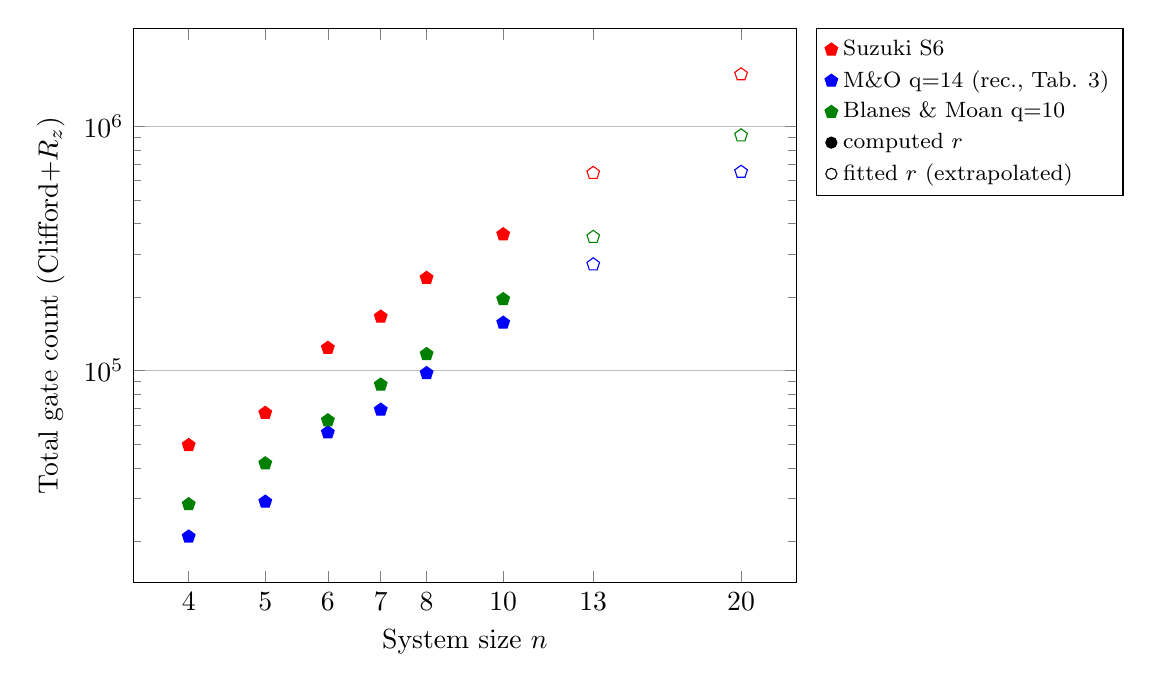
\begin{tikzpicture}
  \begin{loglogaxis}[
    width=10cm,
    xlabel={System size $n$},
    ylabel={Total gate count (Clifford+$R_z$)},
    xtick={4,5,6,7,8,10,13,20},
    xticklabels={4,5,6,7,8,10,13,20},
    ymajorgrids=true,
    legend pos=outer north east,
    legend cell align=left,
    legend style={font=\footnotesize},
  ]
    \addplot[only marks, red, mark=pentagon*, mark size=2.4pt, mark options={solid, fill=red}] coordinates {
      (4,49536)
      (5,67080)
      (6,123840)
      (7,166152)
      (8,239424)
      (10,361200)
    };
    \addlegendentry{Suzuki S6}
    % r from power-law fit (extrapolation); one legend entry per series
    \addplot[only marks, red, mark=pentagon*, mark size=2.4pt, mark options={solid, fill=white}, forget plot] coordinates {
      (13,643968)
      (20,1630560)
    };
    \addplot[only marks, blue, mark=pentagon*, mark size=2.4pt, mark options={solid, fill=blue}] coordinates {
      (4,20916)
      (5,29050)
      (6,55776)
      (7,69139)
      (8,97608)
      (10,156870)
    };
    \addlegendentry{M\&O q=14 (rec., Tab. 3)}
    % r from power-law fit (extrapolation); one legend entry per series
    \addplot[only marks, blue, mark=pentagon*, mark size=2.4pt, mark options={solid, fill=white}, forget plot] coordinates {
      (13,271908)
      (20,650720)
    };
    \addplot[only marks, green!50!black, mark=pentagon*, mark size=2.4pt, mark options={solid, fill=green!50!black}] coordinates {
      (4,28356)
      (5,41700)
      (6,62550)
      (7,87570)
      (8,116760)
      (10,195990)
    };
    \addlegendentry{Blanes \& Moan q=10}
    % r from power-law fit (extrapolation); one legend entry per series
    \addplot[only marks, green!50!black, mark=pentagon*, mark size=2.4pt, mark options={solid, fill=white}, forget plot] coordinates {
      (13,352365)
      (20,917400)
    };
    \addlegendimage{only marks, black, mark=*, mark options={fill=black}}
    \addlegendentry{computed $r$}
    \addlegendimage{only marks, black, mark=*, mark options={fill=white}}
    \addlegendentry{fitted $r$ (extrapolated)}
  \end{loglogaxis}
\end{tikzpicture}

\clearpage

\section*{\texttt{total/B-order8-by-formula.tex}}
Every order-8 formula at measured r\par\medskip
% Generated by pysimcount.pffigure -- do not edit; regenerate instead.
% figure: B-order8-by-formula -- Every order-8 formula at measured r
% source: results/np-main/seed1/results.json
% metric=total gatebase=cz merged
% seed=1 t=n template=simcount synth=pygridsynth
% git_commit=01d3c275ceae2840002bd1aaea68f59b987c4975 git_dirty=False
% source_sha256=0dd1c9775f148df550d3d3f68cfeee1d2d060b7913324535bbf1533b52b4d2c2
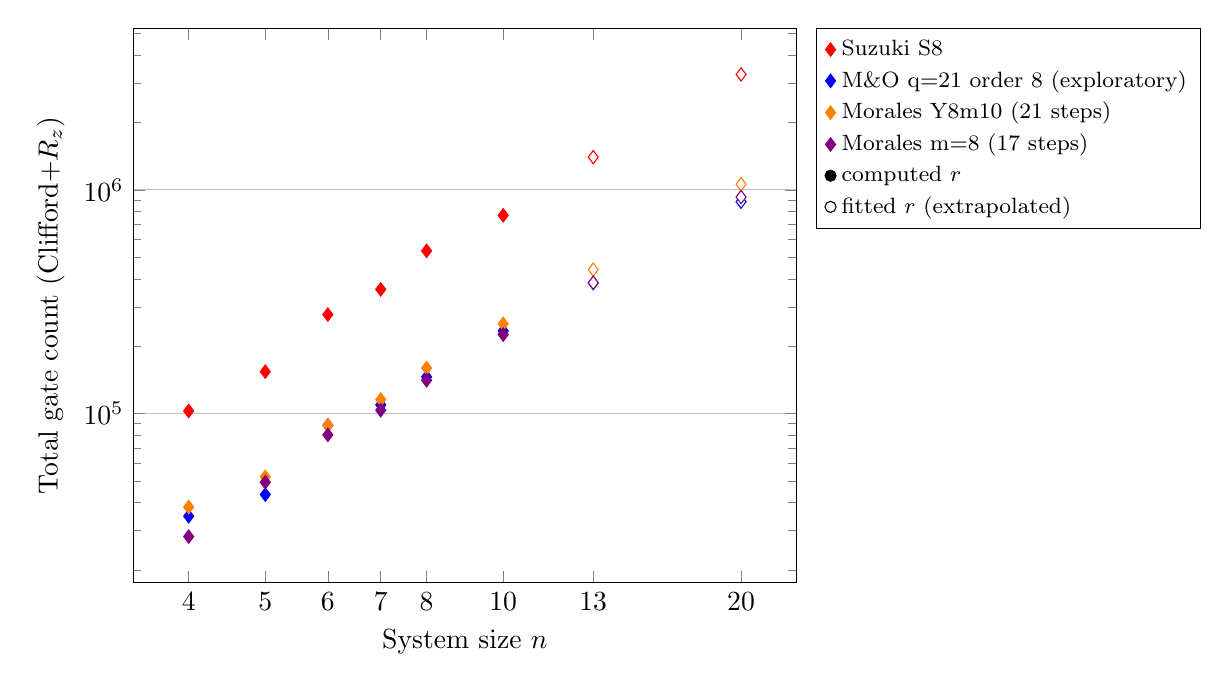
\begin{tikzpicture}
  \begin{loglogaxis}[
    width=10cm,
    xlabel={System size $n$},
    ylabel={Total gate count (Clifford+$R_z$)},
    xtick={4,5,6,7,8,10,13,20},
    xticklabels={4,5,6,7,8,10,13,20},
    ymajorgrids=true,
    legend pos=outer north east,
    legend cell align=left,
    legend style={font=\footnotesize},
  ]
    \addplot[only marks, red, mark=diamond*, mark size=2.4pt, mark options={solid, fill=red}] coordinates {
      (4,102640)
      (5,153960)
      (6,277128)
      (7,359240)
      (8,533728)
      (10,769800)
    };
    \addlegendentry{Suzuki S8}
    % r from power-law fit (extrapolation); one legend entry per series
    \addplot[only marks, red, mark=diamond*, mark size=2.4pt, mark options={solid, fill=white}, forget plot] coordinates {
      (13,1401036)
      (20,3284480)
    };
    \addplot[only marks, blue, mark=diamond*, mark size=2.4pt, mark options={solid, fill=blue}] coordinates {
      (4,34720)
      (5,43400)
      (6,88536)
      (7,109368)
      (8,145824)
      (10,234360)
    };
    \addlegendentry{M\&O q=21 order 8 (exploratory)}
    % r from power-law fit (extrapolation); one legend entry per series
    \addplot[only marks, blue, mark=diamond*, mark size=2.4pt, mark options={solid, fill=white}, forget plot] coordinates {
      (13,383656)
      (20,885360)
    };
    \addplot[only marks, orange, mark=diamond*, mark size=2.4pt, mark options={solid, fill=orange}] coordinates {
      (4,38192)
      (5,52080)
      (6,88536)
      (7,115444)
      (8,159712)
      (10,251720)
    };
    \addlegendentry{Morales Y8m10 (21 steps)}
    % r from power-law fit (extrapolation); one legend entry per series
    \addplot[only marks, orange, mark=diamond*, mark size=2.4pt, mark options={solid, fill=white}, forget plot] coordinates {
      (13,440076)
      (20,1058960)
    };
    \addplot[only marks, violet, mark=diamond*, mark size=2.4pt, mark options={solid, fill=violet}] coordinates {
      (4,28160)
      (5,49280)
      (6,80256)
      (7,103488)
      (8,140800)
      (10,225280)
    };
    \addlegendentry{Morales m=8 (17 steps)}
    % r from power-law fit (extrapolation); one legend entry per series
    \addplot[only marks, violet, mark=diamond*, mark size=2.4pt, mark options={solid, fill=white}, forget plot] coordinates {
      (13,384384)
      (20,929280)
    };
    \addlegendimage{only marks, black, mark=*, mark options={fill=black}}
    \addlegendentry{computed $r$}
    \addlegendimage{only marks, black, mark=*, mark options={fill=white}}
    \addlegendentry{fitted $r$ (extrapolated)}
  \end{loglogaxis}
\end{tikzpicture}

\clearpage

\section*{\texttt{total/B-all-by-formula.tex}}
Every formula at measured r\par\medskip
% Generated by pysimcount.pffigure -- do not edit; regenerate instead.
% figure: B-all-by-formula -- Every formula at measured r
% source: results/np-main/seed1/results.json
% metric=total gatebase=cz merged
% seed=1 t=n template=simcount synth=pygridsynth
% git_commit=01d3c275ceae2840002bd1aaea68f59b987c4975 git_dirty=False
% source_sha256=0dd1c9775f148df550d3d3f68cfeee1d2d060b7913324535bbf1533b52b4d2c2
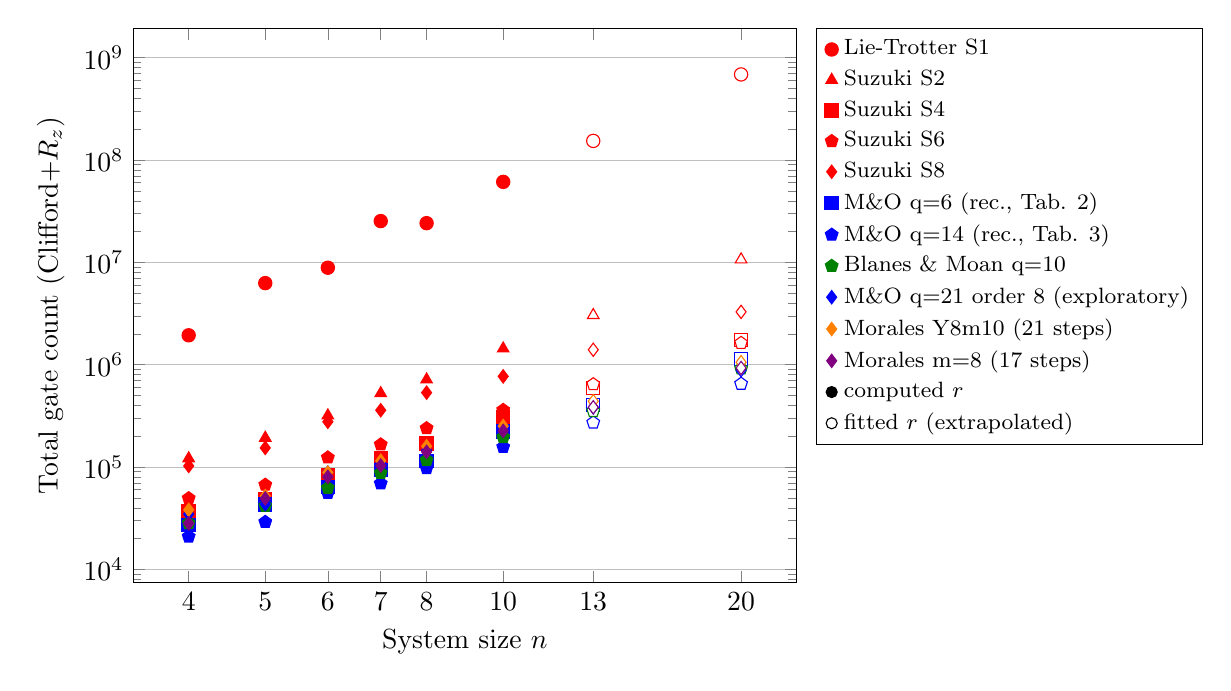
\begin{tikzpicture}
  \begin{loglogaxis}[
    width=10cm,
    xlabel={System size $n$},
    ylabel={Total gate count (Clifford+$R_z$)},
    xtick={4,5,6,7,8,10,13,20},
    xticklabels={4,5,6,7,8,10,13,20},
    ymajorgrids=true,
    legend pos=outer north east,
    legend cell align=left,
    legend style={font=\footnotesize},
  ]
    \addplot[only marks, red, mark=*, mark size=2.4pt, mark options={solid, fill=red}] coordinates {
      (4,1939704)
      (5,6273410)
      (6,8873592)
      (7,25339496)
      (8,24174384)
      (10,61219080)
    };
    \addlegendentry{Lie-Trotter S1}
    % r from power-law fit (extrapolation); one legend entry per series
    \addplot[only marks, red, mark=*, mark size=2.4pt, mark options={solid, fill=white}, forget plot] coordinates {
      (13,153917426)
      (20,686838880)
    };
    \addplot[only marks, red, mark=triangle*, mark size=2.4pt, mark options={solid, fill=red}] coordinates {
      (4,121344)
      (5,192720)
      (6,318816)
      (7,525168)
      (8,715392)
      (10,1437120)
    };
    \addlegendentry{Suzuki S2}
    % r from power-law fit (extrapolation); one legend entry per series
    \addplot[only marks, red, mark=triangle*, mark size=2.4pt, mark options={solid, fill=white}, forget plot] coordinates {
      (13,3051360)
      (20,10674240)
    };
    \addplot[only marks, red, mark=square*, mark size=2.4pt, mark options={solid, fill=red}] coordinates {
      (4,37312)
      (5,48760)
      (6,83952)
      (7,121688)
      (8,169600)
      (10,305280)
    };
    \addlegendentry{Suzuki S4}
    % r from power-law fit (extrapolation); one legend entry per series
    \addplot[only marks, red, mark=square*, mark size=2.4pt, mark options={solid, fill=white}, forget plot] coordinates {
      (13,589784)
      (20,1746880)
    };
    \addplot[only marks, red, mark=pentagon*, mark size=2.4pt, mark options={solid, fill=red}] coordinates {
      (4,49536)
      (5,67080)
      (6,123840)
      (7,166152)
      (8,239424)
      (10,361200)
    };
    \addlegendentry{Suzuki S6}
    % r from power-law fit (extrapolation); one legend entry per series
    \addplot[only marks, red, mark=pentagon*, mark size=2.4pt, mark options={solid, fill=white}, forget plot] coordinates {
      (13,643968)
      (20,1630560)
    };
    \addplot[only marks, red, mark=diamond*, mark size=2.4pt, mark options={solid, fill=red}] coordinates {
      (4,102640)
      (5,153960)
      (6,277128)
      (7,359240)
      (8,533728)
      (10,769800)
    };
    \addlegendentry{Suzuki S8}
    % r from power-law fit (extrapolation); one legend entry per series
    \addplot[only marks, red, mark=diamond*, mark size=2.4pt, mark options={solid, fill=white}, forget plot] coordinates {
      (13,1401036)
      (20,3284480)
    };
    \addplot[only marks, blue, mark=square*, mark size=2.4pt, mark options={solid, fill=blue}] coordinates {
      (4,27324)
      (5,43010)
      (6,63756)
      (7,93863)
      (8,115368)
      (10,222640)
    };
    \addlegendentry{M\&O q=6 (rec., Tab. 2)}
    % r from power-law fit (extrapolation); one legend entry per series
    \addplot[only marks, blue, mark=square*, mark size=2.4pt, mark options={solid, fill=white}, forget plot] coordinates {
      (13,404547)
      (20,1138500)
    };
    \addplot[only marks, blue, mark=pentagon*, mark size=2.4pt, mark options={solid, fill=blue}] coordinates {
      (4,20916)
      (5,29050)
      (6,55776)
      (7,69139)
      (8,97608)
      (10,156870)
    };
    \addlegendentry{M\&O q=14 (rec., Tab. 3)}
    % r from power-law fit (extrapolation); one legend entry per series
    \addplot[only marks, blue, mark=pentagon*, mark size=2.4pt, mark options={solid, fill=white}, forget plot] coordinates {
      (13,271908)
      (20,650720)
    };
    \addplot[only marks, green!50!black, mark=pentagon*, mark size=2.4pt, mark options={solid, fill=green!50!black}] coordinates {
      (4,28356)
      (5,41700)
      (6,62550)
      (7,87570)
      (8,116760)
      (10,195990)
    };
    \addlegendentry{Blanes \& Moan q=10}
    % r from power-law fit (extrapolation); one legend entry per series
    \addplot[only marks, green!50!black, mark=pentagon*, mark size=2.4pt, mark options={solid, fill=white}, forget plot] coordinates {
      (13,352365)
      (20,917400)
    };
    \addplot[only marks, blue, mark=diamond*, mark size=2.4pt, mark options={solid, fill=blue}] coordinates {
      (4,34720)
      (5,43400)
      (6,88536)
      (7,109368)
      (8,145824)
      (10,234360)
    };
    \addlegendentry{M\&O q=21 order 8 (exploratory)}
    % r from power-law fit (extrapolation); one legend entry per series
    \addplot[only marks, blue, mark=diamond*, mark size=2.4pt, mark options={solid, fill=white}, forget plot] coordinates {
      (13,383656)
      (20,885360)
    };
    \addplot[only marks, orange, mark=diamond*, mark size=2.4pt, mark options={solid, fill=orange}] coordinates {
      (4,38192)
      (5,52080)
      (6,88536)
      (7,115444)
      (8,159712)
      (10,251720)
    };
    \addlegendentry{Morales Y8m10 (21 steps)}
    % r from power-law fit (extrapolation); one legend entry per series
    \addplot[only marks, orange, mark=diamond*, mark size=2.4pt, mark options={solid, fill=white}, forget plot] coordinates {
      (13,440076)
      (20,1058960)
    };
    \addplot[only marks, violet, mark=diamond*, mark size=2.4pt, mark options={solid, fill=violet}] coordinates {
      (4,28160)
      (5,49280)
      (6,80256)
      (7,103488)
      (8,140800)
      (10,225280)
    };
    \addlegendentry{Morales m=8 (17 steps)}
    % r from power-law fit (extrapolation); one legend entry per series
    \addplot[only marks, violet, mark=diamond*, mark size=2.4pt, mark options={solid, fill=white}, forget plot] coordinates {
      (13,384384)
      (20,929280)
    };
    \addlegendimage{only marks, black, mark=*, mark options={fill=black}}
    \addlegendentry{computed $r$}
    \addlegendimage{only marks, black, mark=*, mark options={fill=white}}
    \addlegendentry{fitted $r$ (extrapolated)}
  \end{loglogaxis}
\end{tikzpicture}

\clearpage

\section*{\texttt{total/C-lie-trotter-by-bound.tex}}
Lie-Trotter S1: r from each bound and measured\par\medskip
% Generated by pysimcount.pffigure -- do not edit; regenerate instead.
% figure: C-lie-trotter-by-bound -- Lie-Trotter S1: r from each bound and measured
% source: results/np-main/seed1/results.json
% metric=total gatebase=cz merged
% seed=1 t=n template=simcount synth=pygridsynth
% git_commit=01d3c275ceae2840002bd1aaea68f59b987c4975 git_dirty=False
% source_sha256=0dd1c9775f148df550d3d3f68cfeee1d2d060b7913324535bbf1533b52b4d2c2
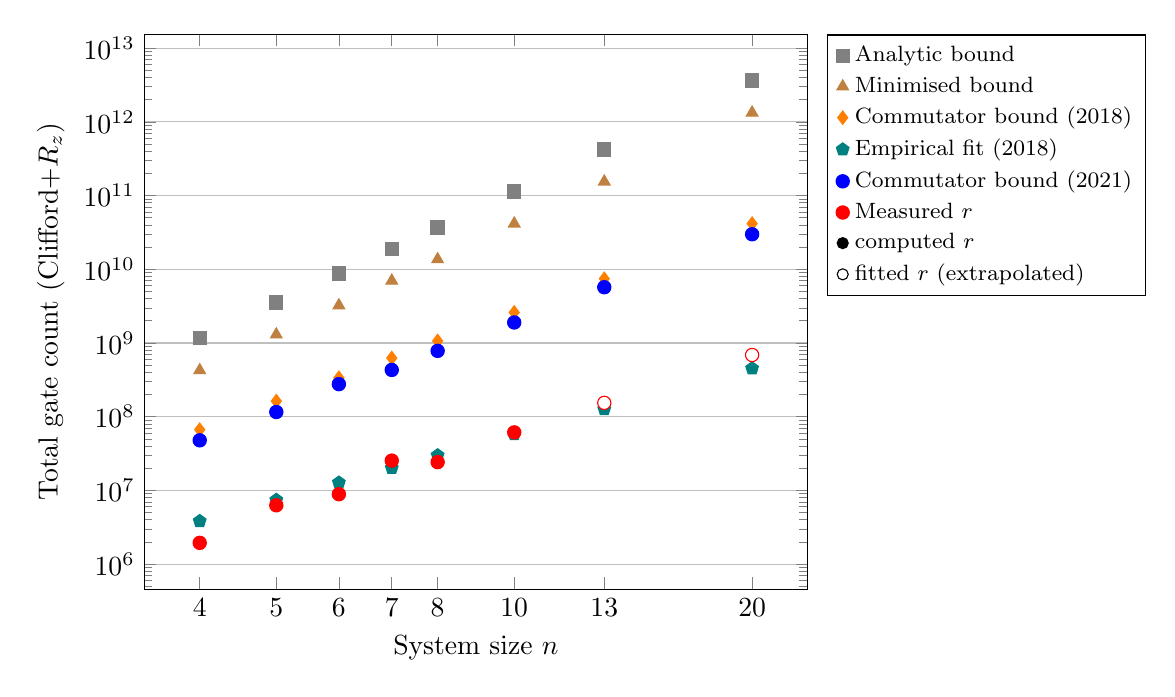
\begin{tikzpicture}
  \begin{loglogaxis}[
    width=10cm,
    xlabel={System size $n$},
    ylabel={Total gate count (Clifford+$R_z$)},
    xtick={4,5,6,7,8,10,13,20},
    xticklabels={4,5,6,7,8,10,13,20},
    ymajorgrids=true,
    legend pos=outer north east,
    legend cell align=left,
    legend style={font=\footnotesize},
  ]
    \addplot[only marks, gray, mark=square*, mark size=2.4pt, mark options={solid, fill=gray}] coordinates {
      (4,1157944632)
      (5,3533766470)
      (6,8793141552)
      (7,19005443730)
      (8,37054226144)
      (10,113080524180)
      (13,419860070266)
      (20,3618576770120)
    };
    \addlegendentry{Analytic bound}
    \addplot[only marks, brown, mark=triangle*, mark size=2.4pt, mark options={solid, fill=brown}] coordinates {
      (4,425990656)
      (5,1300013000)
      (6,3234838464)
      (7,6991747672)
      (8,13631541248)
      (10,41600104000)
      (13,154458116488)
      (20,1331200832000)
    };
    \addlegendentry{Minimised bound}
    \addplot[only marks, orange, mark=diamond*, mark size=2.4pt, mark options={solid, fill=orange}] coordinates {
      (4,66574248)
      (5,162534710)
      (6,337031916)
      (7,624393224)
      (8,1065187344)
      (10,2600554580)
      (13,7427444206)
      (20,41608873280)
    };
    \addlegendentry{Commutator bound (2018)}
    \addplot[only marks, teal, mark=pentagon*, mark size=2.4pt, mark options={solid, fill=teal}] coordinates {
      (4,3826576)
      (5,7413900)
      (6,12727572)
      (7,20098988)
      (8,29857984)
      (10,57850000)
      (13,125901958)
      (20,451398480)
    };
    \addlegendentry{Empirical fit (2018)}
    \addplot[only marks, blue, mark=oplus*, mark size=2.4pt, mark options={solid, fill=blue}] coordinates {
      (4,47754616)
      (5,115578970)
      (6,276106740)
      (7,430452022)
      (8,781371760)
      (10,1897292540)
      (13,5702423688)
      (20,29845046920)
    };
    \addlegendentry{Commutator bound (2021)}
    \addplot[only marks, red, mark=*, mark size=2.4pt, mark options={solid, fill=red}] coordinates {
      (4,1939704)
      (5,6273410)
      (6,8873592)
      (7,25339496)
      (8,24174384)
      (10,61219080)
    };
    \addlegendentry{Measured $r$}
    % r from power-law fit (extrapolation); one legend entry per series
    \addplot[only marks, red, mark=*, mark size=2.4pt, mark options={solid, fill=white}, forget plot] coordinates {
      (13,153917426)
      (20,686838880)
    };
    \addlegendimage{only marks, black, mark=*, mark options={fill=black}}
    \addlegendentry{computed $r$}
    \addlegendimage{only marks, black, mark=*, mark options={fill=white}}
    \addlegendentry{fitted $r$ (extrapolated)}
  \end{loglogaxis}
\end{tikzpicture}

\clearpage

\section*{\texttt{total/C-suzuki2-by-bound.tex}}
Suzuki S2: r from each bound and measured\par\medskip
% Generated by plsimcount.pffigure -- do not edit; regenerate instead.
% figure: C-suzuki2-by-bound -- Suzuki S2: r from each bound and measured
% source: results/np-main/seed1/results.json
% metric=total gatebase=cz merged
% seed=1 t=n template=simcount synth=pygridsynth
% git_commit=01d3c275ceae2840002bd1aaea68f59b987c4975 git_dirty=False
% source_sha256=0dd1c9775f148df550d3d3f68cfeee1d2d060b7913324535bbf1533b52b4d2c2
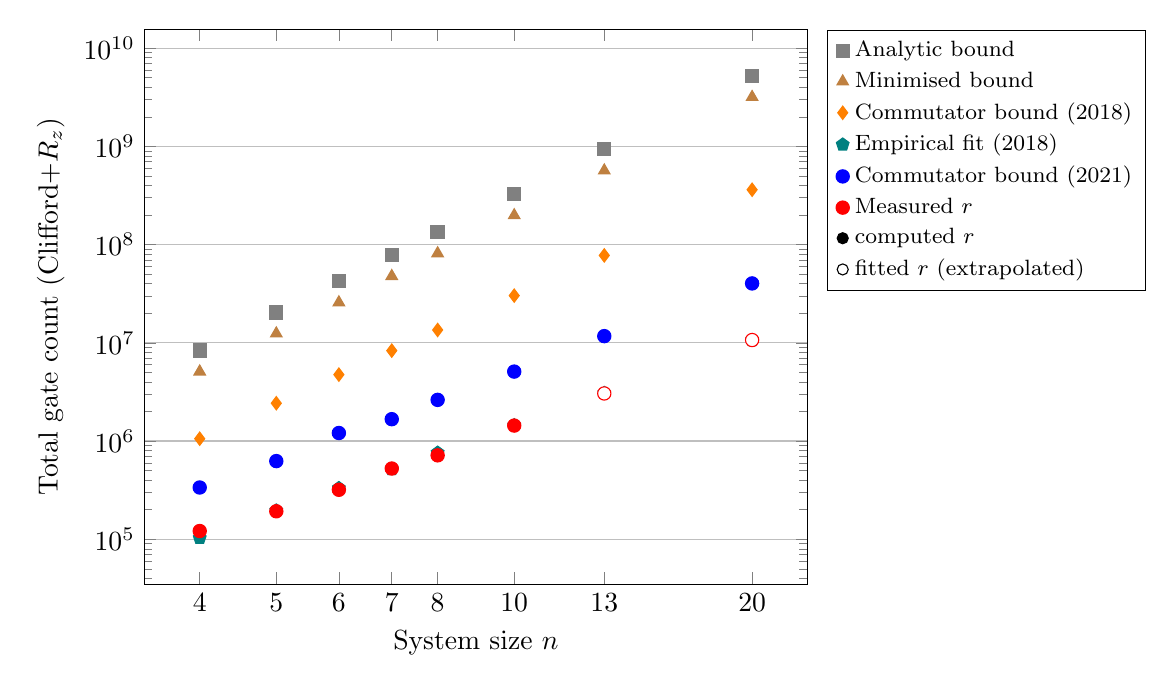
\begin{tikzpicture}
  \begin{loglogaxis}[
    width=10cm,
    xlabel={System size $n$},
    ylabel={Total gate count (Clifford+$R_z$)},
    xtick={4,5,6,7,8,10,13,20},
    xticklabels={4,5,6,7,8,10,13,20},
    ymajorgrids=true,
    legend pos=outer north east,
    legend cell align=left,
    legend style={font=\footnotesize},
  ]
    \addplot[only marks, gray, mark=square*, mark size=2.4pt, mark options={solid, fill=gray}] coordinates {
      (4,8369664)
      (5,20433600)
      (6,42371136)
      (7,78497664)
      (8,133913088)
      (10,326936160)
      (13,933762336)
      (20,5230977600)
    };
    \addlegendentry{Analytic bound}
    \addplot[only marks, brown, mark=triangle*, mark size=2.4pt, mark options={solid, fill=brown}] coordinates {
      (4,5088768)
      (5,12417600)
      (6,25740864)
      (7,47677056)
      (8,81320832)
      (10,198489120)
      (13,566777328)
      (20,3174284160)
    };
    \addlegendentry{Minimised bound}
    \addplot[only marks, orange, mark=diamond*, mark size=2.4pt, mark options={solid, fill=orange}] coordinates {
      (4,1056576)
      (5,2426400)
      (6,4743648)
      (7,8324064)
      (8,13512960)
      (10,30239040)
      (13,77585040)
      (20,361881600)
    };
    \addlegendentry{Commutator bound (2018)}
    \addplot[only marks, teal, mark=pentagon*, mark size=2.4pt, mark options={solid, fill=teal}] coordinates {
      (4,103104)
      (5,196080)
      (6,331776)
      (7,517440)
      (8,760320)
      (10,1446240)
      (13,3080688)
      (20,10664640)
    };
    \addlegendentry{Empirical fit (2018)}
    \addplot[only marks, blue, mark=oplus*, mark size=2.4pt, mark options={solid, fill=blue}] coordinates {
      (4,336576)
      (5,624960)
      (6,1207296)
      (7,1669584)
      (8,2625024)
      (10,5094240)
      (13,11694384)
      (20,40241280)
    };
    \addlegendentry{Commutator bound (2021)}
    \addplot[only marks, red, mark=*, mark size=2.4pt, mark options={solid, fill=red}] coordinates {
      (4,121344)
      (5,192720)
      (6,318816)
      (7,525168)
      (8,715392)
      (10,1437120)
    };
    \addlegendentry{Measured $r$}
    % r from power-law fit (extrapolation); one legend entry per series
    \addplot[only marks, red, mark=*, mark size=2.4pt, mark options={solid, fill=white}, forget plot] coordinates {
      (13,3051360)
      (20,10674240)
    };
    \addlegendimage{only marks, black, mark=*, mark options={fill=black}}
    \addlegendentry{computed $r$}
    \addlegendimage{only marks, black, mark=*, mark options={fill=white}}
    \addlegendentry{fitted $r$ (extrapolated)}
  \end{loglogaxis}
\end{tikzpicture}

\clearpage

\section*{\texttt{total/C-suzuki4-by-bound.tex}}
Suzuki S4: r from each bound and measured\par\medskip
% Generated by plsimcount.pffigure -- do not edit; regenerate instead.
% figure: C-suzuki4-by-bound -- Suzuki S4: r from each bound and measured
% source: results/np-main/seed1/results.json
% metric=total gatebase=cz merged
% seed=1 t=n template=simcount synth=pygridsynth
% git_commit=01d3c275ceae2840002bd1aaea68f59b987c4975 git_dirty=False
% source_sha256=0dd1c9775f148df550d3d3f68cfeee1d2d060b7913324535bbf1533b52b4d2c2
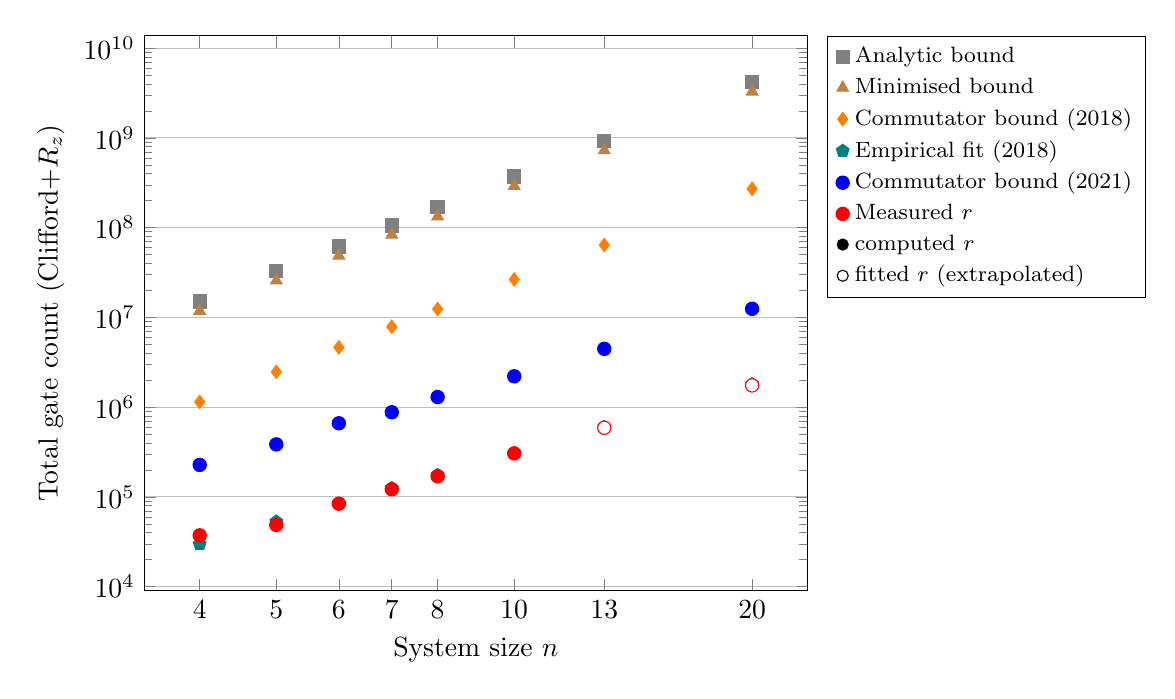
\begin{tikzpicture}
  \begin{loglogaxis}[
    width=10cm,
    xlabel={System size $n$},
    ylabel={Total gate count (Clifford+$R_z$)},
    xtick={4,5,6,7,8,10,13,20},
    xticklabels={4,5,6,7,8,10,13,20},
    ymajorgrids=true,
    legend pos=outer north east,
    legend cell align=left,
    legend style={font=\footnotesize},
  ]
    \addplot[only marks, gray, mark=square*, mark size=2.4pt, mark options={solid, fill=gray}] coordinates {
      (4,14977376)
      (5,32704180)
      (6,61906968)
      (7,106181684)
      (8,169442272)
      (10,370003600)
      (13,926842800)
      (20,4186096880)
    };
    \addlegendentry{Analytic bound}
    \addplot[only marks, brown, mark=triangle*, mark size=2.4pt, mark options={solid, fill=brown}] coordinates {
      (4,11799072)
      (5,25733620)
      (6,48669264)
      (7,83418608)
      (8,133042720)
      (10,290270400)
      (13,726470576)
      (20,3277053600)
    };
    \addlegendentry{Minimised bound}
    \addplot[only marks, orange, mark=diamond*, mark size=2.4pt, mark options={solid, fill=orange}] coordinates {
      (4,1143952)
      (5,2475100)
      (6,4635168)
      (7,7862232)
      (8,12404544)
      (10,26468200)
      (13,64126608)
      (20,270766400)
    };
    \addlegendentry{Commutator bound (2018)}
    \addplot[only marks, teal, mark=pentagon*, mark size=2.4pt, mark options={solid, fill=teal}] coordinates {
      (4,29680)
      (5,53000)
      (6,83952)
      (7,124656)
      (8,174688)
      (10,307400)
      (13,600808)
      (20,1802000)
    };
    \addlegendentry{Empirical fit (2018)}
    \addplot[only marks, blue, mark=oplus*, mark size=2.4pt, mark options={solid, fill=blue}] coordinates {
      (4,227264)
      (5,384780)
      (6,661440)
      (7,877044)
      (8,1297440)
      (10,2206920)
      (13,4464720)
      (20,12465600)
    };
    \addlegendentry{Commutator bound (2021)}
    \addplot[only marks, red, mark=*, mark size=2.4pt, mark options={solid, fill=red}] coordinates {
      (4,37312)
      (5,48760)
      (6,83952)
      (7,121688)
      (8,169600)
      (10,305280)
    };
    \addlegendentry{Measured $r$}
    % r from power-law fit (extrapolation); one legend entry per series
    \addplot[only marks, red, mark=*, mark size=2.4pt, mark options={solid, fill=white}, forget plot] coordinates {
      (13,589784)
      (20,1746880)
    };
    \addlegendimage{only marks, black, mark=*, mark options={fill=black}}
    \addlegendentry{computed $r$}
    \addlegendimage{only marks, black, mark=*, mark options={fill=white}}
    \addlegendentry{fitted $r$ (extrapolated)}
  \end{loglogaxis}
\end{tikzpicture}

\clearpage

\section*{\texttt{total/C-suzuki6-by-bound.tex}}
Suzuki S6: r from each bound and measured\par\medskip
% Generated by plsimcount.pffigure -- do not edit; regenerate instead.
% figure: C-suzuki6-by-bound -- Suzuki S6: r from each bound and measured
% source: results/np-main/seed1/results.json
% metric=total gatebase=cz merged
% seed=1 t=n template=simcount synth=pygridsynth
% git_commit=01d3c275ceae2840002bd1aaea68f59b987c4975 git_dirty=False
% source_sha256=0dd1c9775f148df550d3d3f68cfeee1d2d060b7913324535bbf1533b52b4d2c2
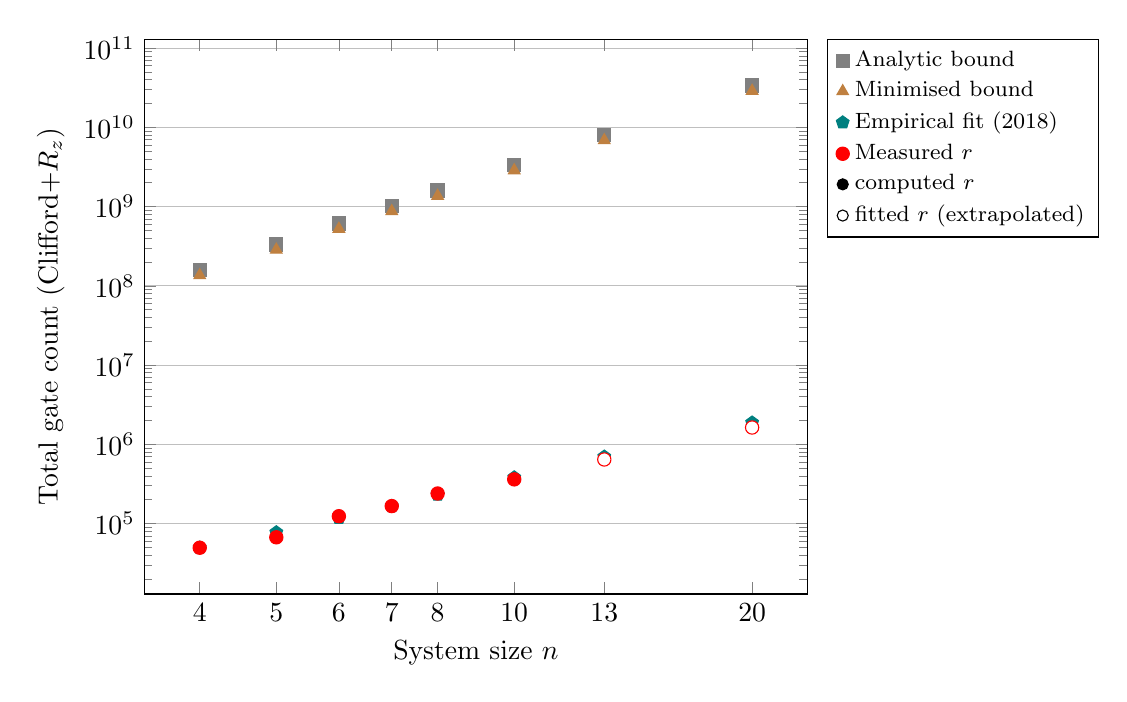
\begin{tikzpicture}
  \begin{loglogaxis}[
    width=10cm,
    xlabel={System size $n$},
    ylabel={Total gate count (Clifford+$R_z$)},
    xtick={4,5,6,7,8,10,13,20},
    xticklabels={4,5,6,7,8,10,13,20},
    ymajorgrids=true,
    legend pos=outer north east,
    legend cell align=left,
    legend style={font=\footnotesize},
  ]
    \addplot[only marks, gray, mark=square*, mark size=2.4pt, mark options={solid, fill=gray}] coordinates {
      (4,157743264)
      (5,331880880)
      (6,609422832)
      (7,1018757376)
      (8,1589932224)
      (10,3345114480)
      (13,8020876344)
      (20,33716595840)
    };
    \addlegendentry{Analytic bound}
    \addplot[only marks, brown, mark=triangle*, mark size=2.4pt, mark options={solid, fill=brown}] coordinates {
      (4,135712128)
      (5,285198360)
      (6,523242576)
      (7,874082328)
      (8,1363346304)
      (10,2865771120)
      (13,6864685464)
      (20,28814368800)
    };
    \addlegendentry{Minimised bound}
    \addplot[only marks, teal, mark=pentagon*, mark size=2.4pt, mark options={solid, fill=teal}] coordinates {
      (4,49536)
      (5,77400)
      (6,117648)
      (7,166152)
      (8,231168)
      (10,381840)
      (13,697632)
      (20,1878240)
    };
    \addlegendentry{Empirical fit (2018)}
    \addplot[only marks, red, mark=*, mark size=2.4pt, mark options={solid, fill=red}] coordinates {
      (4,49536)
      (5,67080)
      (6,123840)
      (7,166152)
      (8,239424)
      (10,361200)
    };
    \addlegendentry{Measured $r$}
    % r from power-law fit (extrapolation); one legend entry per series
    \addplot[only marks, red, mark=*, mark size=2.4pt, mark options={solid, fill=white}, forget plot] coordinates {
      (13,643968)
      (20,1630560)
    };
    \addlegendimage{only marks, black, mark=*, mark options={fill=black}}
    \addlegendentry{computed $r$}
    \addlegendimage{only marks, black, mark=*, mark options={fill=white}}
    \addlegendentry{fitted $r$ (extrapolated)}
  \end{loglogaxis}
\end{tikzpicture}

\clearpage

\section*{\texttt{total/C-suzuki8-by-bound.tex}}
Suzuki S8: r from each bound and measured\par\medskip
% Generated by pysimcount.pffigure -- do not edit; regenerate instead.
% figure: C-suzuki8-by-bound -- Suzuki S8: r from each bound and measured
% source: results/np-main/seed1/results.json
% metric=total gatebase=cz merged
% seed=1 t=n template=simcount synth=pygridsynth
% git_commit=01d3c275ceae2840002bd1aaea68f59b987c4975 git_dirty=False
% source_sha256=0dd1c9775f148df550d3d3f68cfeee1d2d060b7913324535bbf1533b52b4d2c2
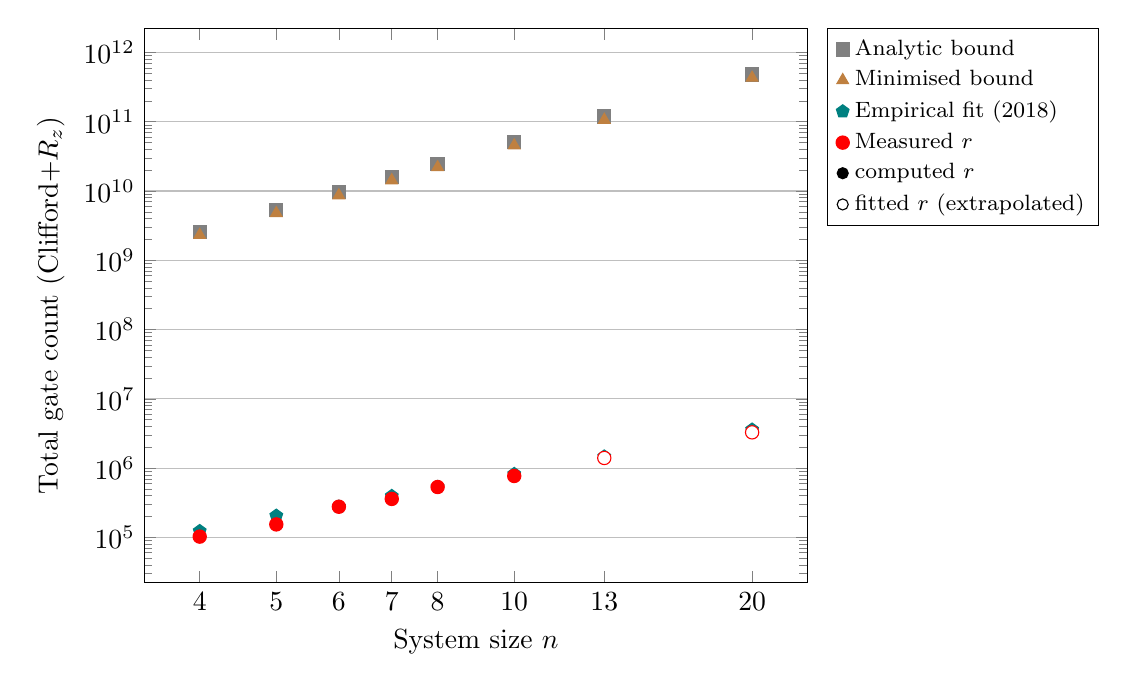
\begin{tikzpicture}
  \begin{loglogaxis}[
    width=10cm,
    xlabel={System size $n$},
    ylabel={Total gate count (Clifford+$R_z$)},
    xtick={4,5,6,7,8,10,13,20},
    xticklabels={4,5,6,7,8,10,13,20},
    ymajorgrids=true,
    legend pos=outer north east,
    legend cell align=left,
    legend style={font=\footnotesize},
  ]
    \addplot[only marks, gray, mark=square*, mark size=2.4pt, mark options={solid, fill=gray}] coordinates {
      (4,2580061680)
      (5,5328273340)
      (6,9636633528)
      (7,15903842192)
      (8,24545740160)
      (10,50691330000)
      (13,118918467928)
      (20,482259582560)
    };
    \addlegendentry{Analytic bound}
    \addplot[only marks, brown, mark=triangle*, mark size=2.4pt, mark options={solid, fill=brown}] coordinates {
      (4,2317590672)
      (5,4781715340)
      (6,8641774800)
      (7,14253457708)
      (8,21987540800)
      (10,45371909360)
      (13,106345237284)
      (20,430694067680)
    };
    \addlegendentry{Minimised bound}
    \addplot[only marks, teal, mark=pentagon*, mark size=2.4pt, mark options={solid, fill=teal}] coordinates {
      (4,123168)
      (5,205280)
      (6,277128)
      (7,395164)
      (8,533728)
      (10,821120)
      (13,1467752)
      (20,3592400)
    };
    \addlegendentry{Empirical fit (2018)}
    \addplot[only marks, red, mark=*, mark size=2.4pt, mark options={solid, fill=red}] coordinates {
      (4,102640)
      (5,153960)
      (6,277128)
      (7,359240)
      (8,533728)
      (10,769800)
    };
    \addlegendentry{Measured $r$}
    % r from power-law fit (extrapolation); one legend entry per series
    \addplot[only marks, red, mark=*, mark size=2.4pt, mark options={solid, fill=white}, forget plot] coordinates {
      (13,1401036)
      (20,3284480)
    };
    \addlegendimage{only marks, black, mark=*, mark options={fill=black}}
    \addlegendentry{computed $r$}
    \addlegendimage{only marks, black, mark=*, mark options={fill=white}}
    \addlegendentry{fitted $r$ (extrapolated)}
  \end{loglogaxis}
\end{tikzpicture}

\clearpage
\end{document}
